\documentclass[11pt]{extarticle}
\usepackage[letterpaper,margin=1.0in]{geometry}
%% Load our math packages
\usepackage{amsmath,amssymb,amsfonts,amsthm}
\usepackage{xfrac} % Allow sidways fractions num/denom
\usepackage{mathtools} % Allow multiline equations
\usepackage[font=footnotesize]{caption}
\usepackage{url}
\usepackage{cancel}
\usepackage{subcaption} % used for subfigure side by sides
\usepackage{multicol}
\usepackage{graphicx}
\usepackage{epstopdf}
\usepackage{bm}
%% Load TIKZ for drawing figures
\usepackage{tikz}
\usetikzlibrary{positioning}
\usetikzlibrary{shapes,snakes}
%% Load core packages we need
\usepackage{algorithm}% http://ctan.org/pkg/algorithms
% \usepackage{algorithmic} % algorithms!!
\usepackage{algpseudocode}% http://ctan.org/pkg/algorithmicx
\usepackage{lipsum} % for generated text
\usepackage{empheq} % Boxed equations http://tex.stackexchange.com/a/14298
\usepackage{xcolor} % Boxed equations http://tex.stackexchange.com/a/14298
\usepackage{fancyhdr} % Allow for nice footers
\pagestyle{fancy} % Allow for nice footers
\usepackage{tabulary} % allow tables with line breaks
\usepackage{enumitem} % allows for removal of list spacing
\usepackage[colorlinks]{hyperref} % allow url links (REMOVE "colorlinks" IF PRINTING)
\usepackage{float} % allow using of [H] tag on "figure"s
\usepackage{color} % color text package
\usepackage[titletoc,title]{appendix} % appendix
\usepackage[backend=bibtex,sorting=none]{biblatex}
\bibliography{libraries/extras,libraries/library}
\graphicspath{{figures/}}
\DeclareGraphicsExtensions{.PNG,.JPG,.pdf,.png,.jpg,.jpeg}
%
% Clear the headers and footers
\fancyhf{}
\renewcommand{\headrulewidth}{0pt}
%
%
% Allow more then 10 columns in matrix
\setcounter{MaxMatrixCols}{20}
%
% Fix appendix titles
\usepackage{etoolbox}
\patchcmd{\appendices}{\quad}{: }{}{}
%
% Custom references (used in the rules section)
\makeatletter
\newcommand{\customlabel}[2]{%
   \protected@write \@auxout {}{\string \newlabel {#1}{{#2}{\thepage}{#2}{#1}{}} }%
   \hypertarget{#1}{#2}
}
\makeatother

%%%%%%%%%%%%%%%%%%%%%%%%%%%%%%%%%%%%%%%%%%%%%%%%%%%%%%%%%%%%%%%%%%%%%%%
% CUSTOM COMMANDS
%%%%%%%%%%%%%%%%%%%%%%%%%%%%%%%%%%%%%%%%%%%%%%%%%%%%%%%%%%%%%%%%%%%%%%%
% Custom command to stick things to bottom of pages
\newenvironment{bottompar}{\par\vspace*{\fill}}{\clearpage}
% Better cancel line
% https://tex.stackexchange.com/a/20648
\usepackage{tikz}
\usetikzlibrary{calc}
\usepackage{xparse}
\DeclareDocumentCommand{\hcancel}{mO{0pt}O{0pt}O{0pt}O{0pt}}{%
    \tikz[baseline=(tocancel.base)]{
        \node[inner sep=0pt,outer sep=0pt] (tocancel) {$#1$};
        \draw[red] ($(tocancel.south west)+(#2,#3)$) -- ($(tocancel.north east)+(#4,#5)$);
    }%
}%
% Allow for absolute value and norm brackets
% https://tex.stackexchange.com/a/43009
\DeclarePairedDelimiter\abs{\lvert}{\rvert}%
\DeclarePairedDelimiter\norm{\lVert}{\rVert}%
\newcommand{\skewsym}[1]{\left\lfloor#1\right\rfloor_{\times}}
\newcommand{\vect}[1]{\boldsymbol{\mathbf{#1}}}
% Expectation, reals, and transpose shortcuts used in the lecture notes
\newcommand{\E}{\mathbb{E}}
\newcommand{\Reals}{\mathbb{R}}
\newcommand{\trans}{^\top}
% Lie-group operators used in Lecture 2
\DeclareMathOperator{\Exp}{Exp}
\DeclareMathOperator{\Log}{Log}
\DeclareMathOperator{\Ad}{Ad}
\DeclareMathOperator{\tr}{tr}
% Swap the definition of \abs* and \norm*, so that \abs
% and \norm resizes the size of the brackets, and the 
% starred version does not.
\makeatletter
\let\oldabs\abs
\def\abs{\@ifstar{\oldabs}{\oldabs*}}
\let\oldnorm\norm
\def\norm{\@ifstar{\oldnorm}{\oldnorm*}}
\makeatother

\begin{document}



%%%%%%%%%%%%%%%%%%%%%%%%%%%%%%%%%%%%%%%%%%%%%%%%%%%%%%%%%%%%%%%%%%%%%%%
% Main sections of the report
%%%%%%%%%%%%%%%%%%%%%%%%%%%%%%%%%%%%%%%%%%%%%%%%%%%%%%%%%%%%%%%%%%%%%%%
%
%
\begin{center}
\textcolor[RGB]{180,180,180}{\rule{\linewidth}{0.2pt}}
\end{center}
\vspace*{5mm}
%
% Course banner
%
%\begin{center}
%\large Robotics \& State Estimation (RiSE) Tutorials
%\end{center}
%
% Main Title                                                                
%
\Huge
\begin{center}
Robotics \& State Estimation (RiSE)\\
\end{center}
\normalsize
%
% Instructors
%
{
\hypersetup{
    colorlinks = true,
    allcolors = {black}
}
\vspace{10mm}
\begin{center}
Yulin Yang - \href{mailto:yangyulin1@gmail.com}{yangyulin1@gmail.com} \\
Chuchu Chen - \href{mailto:chuchu.chen@gwu.edu}{chuchu.chen@gwu.edu} \\
Xingxing Zuo - \href{mailto:xingxing.zuo@mbzuai.ac.ae}{xingxing.zuo@mbzuai.ac.ae}
\end{center}
}
%
% Course / affiliation
%
\vspace{10mm}
\begin{center}
%Robotics \& State Estimation Tutorials \\
\url{https://github.com/yangyulin/rise-tutorial}
\end{center}
%
% Bottom of page footer area
%
\begin{bottompar}
%
% Logo
\begin{center}

\includegraphics[height=6cm]{figures/RiSE_v1}
\end{center}
% Bottom text
\begin{center}
\textcolor[RGB]{180,180,180}{\rule{\linewidth}{0.2pt}}
\end{center}
%
%
%Robotics \& State Estimation (RiSE) Tutorials \\
Lecture Notes - RiSE-2026 \\
Last Updated - \today % automatically insert the date
%
\vspace{5cm}
\end{bottompar}
%
% Reset the figure counter
\setcounter{figure}{0}
\newpage
% Do not number this page
\clearpage


% Make table of contents
{
 \hypersetup{
     colorlinks = true,
     allcolors = {black}
 }
\tableofcontents
% Do not number this page
\clearpage
% New page
\newpage
}

% Update the footer
\lfoot{RiSE Tutorials}
\cfoot{}
\rfoot{\thepage}

% Reset the page count to one
\setcounter{page}{1}

%
% One \section per lecture, each starting on a fresh page. Add \input lines here as lectures are added.
\section{Lecture 1: Foundations --- Probability, Linear Algebra, and Linear Systems}
\label{sec:lecture01}

% =====================================================================
\subsection{Probability}

\subsubsection{Definition.}

For an event $A$, the probability $P(A)$ is
\begin{align}
P(A) = \frac{N_A}{N},
\end{align}
where $N_A$ is the number of occurrences of $A$ and $N$ is the number of all possible outcomes.

\subsubsection{Conditional probability.}
The probability of event $A$ given that event $B$ is true is
\begin{align}
P(A\mid B) = \frac{P(A,B)}{P(B)}, \qquad P(B)\neq 0,
\end{align}
which yields the product rule
\begin{align}
P(A,B) & = P(A\mid B)\,P(B)\\
& = P(B\mid A)\,P(A).
\end{align}

\subsubsection{Total probability theorem.}
If $\{A_1,\dots,A_n\}$ is a partition (mutually exclusive, $P(A_i,A_j)=0$ for $i\neq j$) and $B$ is an arbitrary event, then
\begin{align}
P(B) = P(B\mid A_1)P(A_1) + \cdots + P(B\mid A_n)P(A_n) = \sum_{i} P(B\mid A_i)\,P(A_i).
\end{align}

\paragraph{Bayes' theorem.}
\begin{align}
P(A_i\mid B) = \frac{P(B\mid A_i)\,P(A_i)}{P(B)} = \frac{P(B\mid A_i)\,P(A_i)}{\sum_{i} P(B\mid A_i)\,P(A_i)}.
\end{align}

\paragraph{Independence.}
With the inclusion--exclusion relation $P(A\cup B) = P(A) + P(B) - P(A\cap B)$, two events $A$ and $B$ are independent when
\begin{align}
P(A,B) = P(A\mid B)\,P(B) = P(A)\,P(B) = P(B\mid A)\,P(A) = P(B)\,P(A).
\end{align}

% =====================================================================
\subsection{Random Variables}

A random variable defines a function that quantifies an experiment. For a sample space $S=\{s_1,\dots,s_n\}$, a random variable is a map $\mathrm{x}:S\to\Reals$ with $\mathrm{x}(s_i)=x_i$.

\paragraph{Distribution.}
The (cumulative) distribution of a random variable $\mathrm{x}$ is
\begin{align}
F_{\mathrm{x}}(x) = P(\mathrm{x}\le x),
\end{align}
i.e. the probability that $\mathrm{x}$ takes a value lower than or equal to $x$.

\paragraph{Probability density function (pdf).}
\begin{align}
p(x) = \lim_{\varepsilon\to 0}\frac{F_{\mathrm{x}}(x)-F_{\mathrm{x}}(x-\varepsilon)}{\varepsilon} = \frac{\mathrm{d}F_{\mathrm{x}}(x)}{\mathrm{d}x} = \frac{\mathrm{d}P(\mathrm{x}\le x)}{\mathrm{d}x},
\end{align}
hence
\begin{align}
P(\mathrm{x}\le x) = \int_{-\infty}^{x} p(\xi)\,\mathrm{d}\xi, \qquad
P(\mathrm{x}\le\infty) = 1 = \int_{-\infty}^{+\infty} p(\xi)\,\mathrm{d}\xi,
\end{align}
and for an interval
\begin{align}
P(x_1\le \mathrm{x} < x_2) = \int_{x_1}^{x_2} p(\xi)\,\mathrm{d}\xi.
\end{align}

\paragraph{Example distributions.}
\begin{itemize}[itemsep=0.4em]
\item Gaussian: $\mathrm{x}\sim\mathcal{N}(m,\sigma) \;\Longleftrightarrow\; p(x) = \dfrac{1}{\sqrt{2\pi}\,\sigma}\,e^{-\frac{(x-m)^2}{2\sigma^2}}$.
\item Uniform: $p(x) = \begin{cases} 0 & x < x_1 \\[2pt] \dfrac{1}{x_2-x_1} & x_1\le x\le x_2 \\[4pt] 0 & x > x_2 \end{cases}$
\end{itemize}

\paragraph{Conditional distribution and density.}
\begin{align}
P(\mathrm{x}\le x\mid A) = \frac{P(\mathrm{x}\le x,\, A)}{P(A)}, \qquad
p(x\mid A) = \frac{\mathrm{d}P(\mathrm{x}\le x\mid A)}{\mathrm{d}x}.
\end{align}

\paragraph{Total probability theorem for pdfs.}
For a mutually exclusive partition $\{A_1,\dots,A_n\}$,
\begin{align}
p(x) = p(x\mid A_1)P(A_1) + \cdots + p(x\mid A_n)P(A_n).
\end{align}

\paragraph{Continuous Bayes' theorem.}
Using the infinitesimal relations $P(\mathrm{x}=x) = p(x)\,\delta x$ and $P(\mathrm{x}=x\mid A) = p(x\mid A)\,\delta x$,
\begin{align}
P(A\mid \mathrm{x}=x) = \frac{P(A,\, \mathrm{x}=x)}{P(\mathrm{x}=x)}
= \frac{P(\mathrm{x}=x\mid A)\,P(A)}{P(\mathrm{x}=x)}
= \frac{p(x\mid A)}{p(x)}\,P(A),
\end{align}
so that $P(A\mid \mathrm{x}=x)\,p(x) = p(x\mid A)\,P(A)$, which gives the continuous total-probability and Bayes' relations
\begin{align}
P(A) &= \int_{-\infty}^{+\infty} P(A\mid \mathrm{x}=x)\,p(x)\,\mathrm{d}x, \\
p(x\mid A) &= \frac{P(A\mid \mathrm{x}=x)}{P(A)}\,p(x)
= \frac{P(A\mid \mathrm{x}=x)\,p(x)}{\int_{-\infty}^{+\infty} P(A\mid \mathrm{x}=x)\,p(x)\,\mathrm{d}x}.
\end{align}

% =====================================================================
\subsection{Expectation, Variance, and Random Vectors}

\paragraph{Mean.}
The expected value (mean) of a continuous random variable, and its conditional version, are
\begin{align}
m_x = \E(\mathrm{x}) = \int_{-\infty}^{+\infty} x\,p(x)\,\mathrm{d}x, \qquad
m_x = \E(\mathrm{x}\mid A) = \int_{-\infty}^{+\infty} x\,p(x\mid A)\,\mathrm{d}x.
\end{align}

\paragraph{Variance.}
\begin{align}
\sigma_x^2 = \E\big((\mathrm{x}-m_x)^2\big) = \int_{-\infty}^{+\infty}(x-m_x)^2\,p(x)\,\mathrm{d}x = \E(\mathrm{x}^2) - \big(\E(\mathrm{x})\big)^2,
\end{align}
with the conditional variance
\begin{align}
\sigma_{x\mid A}^2 = \E\big\{(\mathrm{x}-m_{x\mid A})^2 \mid A\big\} = \int_{-\infty}^{+\infty}(x-m_{x\mid A})^2\,p(x\mid A)\,\mathrm{d}x.
\end{align}

\paragraph{A set of random variables.}
The joint pdf of $x_1,\dots,x_n$ satisfies
\begin{align}
\int_{-\infty}^{+\infty}\!\!\!\cdots\!\int_{-\infty}^{+\infty} p(x_1,\dots,x_n)\,\mathrm{d}x_1\cdots\mathrm{d}x_n = 1.
\end{align}
If $x_i,x_j$ are independent, $p(x_i,x_j) = p(x_i)\,p(x_j)$. Expectation is linear: for $y = \alpha x_i + \beta x_j$,
\begin{align}
\E(y) = \alpha\,\E(x_i) + \beta\,\E(x_j).
\end{align}

\paragraph{Covariance.}
\begin{align}
\sigma_{ij}^2 = \E\big((x_i-m_i)(x_j-m_j)\big) = \E(x_i x_j) - \E(x_i)\,\E(x_j).
\end{align}
When $\sigma_{ij}=0$ we have $\E(x_i x_j) = \E(x_i)\,\E(x_j)$ and $x_i,x_j$ are \emph{uncorrelated}.

\begin{quote}
\textbf{Discussion questions.}
\begin{enumerate}[itemsep=0.2em]
\item If $x_i,x_j$ are independent, then $p(x_i,x_j)=p(x_i)p(x_j) \Rightarrow \E(x_i x_j)=\E(x_i)\E(x_j)$ --- so independence implies uncorrelated.
\item If $x_i,x_j$ are uncorrelated, are they necessarily independent?
\item If $x_i,x_j$ are jointly Gaussian, is independence equivalent to being uncorrelated?
\end{enumerate}
\end{quote}

\paragraph{Random vector.}
Let $\vect{x} = [x_1,\dots,x_n]\trans$, where all elements are random variables, with mean $\E(\vect{x})\triangleq\vect{m}_x$ and covariance
\begin{align}
\vect{P} = \E\big((\vect{x}-\vect{m}_x)(\vect{x}-\vect{m}_x)\trans\big) = \E(\vect{x}\vect{x}\trans) - \E(\vect{x})\,\E(\vect{x}\trans),
\end{align}
with entries
\begin{align}
P_{ii} = \E\big((x_i-m_i)^2\big) = \int_{-\infty}^{+\infty}(x_i-m_i)^2 p(x_i)\,\mathrm{d}x_i,
\qquad
P_{ij} = \E\big((x_i-m_i)(x_j-m_j)\big).
\end{align}
Since $P_{ij}=P_{ji}$, the covariance $\vect{P}$ is a symmetric matrix; it is also positive (semi-)definite.

\paragraph{Gaussian vector pdf.}
\begin{align}
p(\vect{x}) = \frac{1}{(2\pi)^{n/2}\sqrt{|\vect{P}|}}\,\exp\!\Big(-\tfrac{1}{2}(\vect{x}-\vect{m}_x)\trans \vect{P}^{-1}(\vect{x}-\vect{m}_x)\Big),
\end{align}
where $|\vect{P}|$ is the determinant of $\vect{P}$, $\vect{m}_x=\E(\vect{x})$, and $\vect{P}=\E\big((\vect{x}-\vect{m}_x)(\vect{x}-\vect{m}_x)\trans\big)$.

\begin{quote}
\textbf{Homework.}
Let $\vect{x}=[x_1,\dots,x_n]\trans$ with $p(\vect{x})=\mathcal{N}(\vect{m}_x,\vect{P}_{xx})$. Define
\begin{align*}
q = (\vect{x}-\vect{m}_x)\trans \vect{P}_{xx}^{-1}(\vect{x}-\vect{m}_x),
\qquad
\vect{y} = \vect{P}_{xx}^{-1/2}(\vect{x}-\vect{m}_x), \quad q = \vect{y}\trans\vect{y} = \sum_i y_i^2.
\end{align*}
What are the mean and covariance of $q$?
\end{quote}

% =====================================================================
\subsection{Maximum Likelihood and Maximum a Posteriori Estimation}

For a measurement model with additive noise $z_i = h_i(\vect{x}) + n_i$, stacked as $\vect{z} = \vect{h}(\vect{x}) + \vect{n}$, two estimators are
\begin{itemize}[itemsep=0.3em]
\item \textbf{Maximum likelihood estimation (MLE):} $\displaystyle \max_{\vect{x}}\, p(\vect{z}\mid\vect{x})$.
\item \textbf{Maximum a posteriori (MAP):} $\displaystyle \max_{\vect{x}}\, p(\vect{x}\mid\vect{z})$, with $p(\vect{x}\mid\vect{z}) = \dfrac{p(\vect{z}\mid\vect{x})\,p(\vect{x})}{p(\vect{z})}$.
\end{itemize}

For zero-mean Gaussian noise $\vect{n}\sim\mathcal{N}(\vect{0},\vect{P})$,
\begin{align}
\max_{\vect{x}} p(\vect{z}\mid\vect{x}) = \max_{\vect{x}} \frac{1}{(2\pi)^{n/2}\sqrt{|\vect{P}|}}\,\exp\!\Big(-(\vect{z}-\vect{h}(\vect{x}))\trans \vect{P}^{-1}(\vect{z}-\vect{h}(\vect{x}))\Big),
\end{align}
which is equivalent to the weighted least-squares problem
\begin{align}
\min_{\vect{x}}\; C = (\vect{z}-\vect{h}(\vect{x}))\trans \vect{P}^{-1}(\vect{z}-\vect{h}(\vect{x})).
\end{align}
Linearizing about $\hat{\vect{x}}$ with $\vect{z} = \vect{h}(\vect{x}) + \vect{n} = \vect{h}(\hat{\vect{x}}) + \vect{H}(\vect{x}-\hat{\vect{x}}) + \vect{n}$, and defining the residual $\tilde{\vect{z}} = \vect{z} - \vect{h}(\hat{\vect{x}})$ and error $\tilde{\vect{x}} = \vect{x} - \hat{\vect{x}}$,
\begin{align}
\min_{\tilde{\vect{x}}}\; (\tilde{\vect{z}} - \vect{H}\tilde{\vect{x}})\trans \vect{P}^{-1}(\tilde{\vect{z}} - \vect{H}\tilde{\vect{x}})
= \min_{\tilde{\vect{x}}}\big(\tilde{\vect{z}}\trans\tilde{\vect{z}} - 2\,\tilde{\vect{z}}\trans\vect{P}^{-1}\vect{H}\tilde{\vect{x}} + \tilde{\vect{x}}\trans \vect{H}\trans\vect{P}^{-1}\vect{H}\tilde{\vect{x}}\big).
\end{align}
Setting the gradient to zero gives the normal equations $\vect{H}\trans\vect{P}^{-1}\vect{H}\,\tilde{\vect{x}} = \vect{H}\trans\vect{P}^{-1}\tilde{\vect{z}}$, hence
\begin{empheq}[box=\fbox]{align}
\vect{x}^{\oplus} = \hat{\vect{x}} + \tilde{\vect{x}} = \hat{\vect{x}} + (\vect{H}\trans\vect{P}^{-1}\vect{H})^{-1}\vect{H}\trans\vect{P}^{-1}\tilde{\vect{z}}.
\end{empheq}
This is the classical weighted least-squares solution.

\begin{quote}
\textbf{Questions.}
\begin{enumerate}[itemsep=0.2em]
\item What is the covariance of the new estimate $\vect{x}^{\oplus}$?
\item For a prior $\vect{x}_p = \vect{x} + \vect{n}_p$ together with $z_i = h_i(\vect{x}) + n_i$, $i=1,\dots,n$, what is the MAP solution $\max_{\vect{x}} p(\vect{x}\mid\vect{z})$?
\end{enumerate}
\end{quote}

\paragraph{Optimization.}
Nonlinear least-squares problems are solved iteratively, e.g. Gauss--Newton (GN) and Levenberg--Marquardt (LM).

% =====================================================================
\subsection{Linear Systems}

A linear (continuous-time) state-space system is
\begin{align}
\dot{\vect{x}} = \vect{A}\vect{x} + \vect{B}\vect{u}, \qquad \vect{y} = \vect{C}\vect{x} + \vect{D}\vect{u},
\end{align}
where $\vect{x}$ is the state, $\vect{u}$ the input, and $\vect{y}$ the output. Its discrete-time counterpart is
\begin{align}
\vect{x}_{k+1} = \vect{A}'\vect{x}_k + \vect{B}'\vect{u}_k, \qquad \vect{y}_{k+1} = \vect{C}'\vect{x}_{k+1} + \vect{D}'\vect{u}_{k+1}.
\end{align}
If $\vect{A},\vect{B},\vect{C},\vect{D}$ are constant, the system is \emph{linear time-invariant} (LTI); if they depend on time, it is \emph{linear time-variant} (LTV).

\paragraph{Homogeneous solution.}
Consider $\dot{\vect{x}} = \vect{A}\vect{x}$ with $\vect{x}(t_0)=\vect{x}_0$ and $\vect{y} = \vect{C}\vect{x}$. From $\dot{\vect{x}} - \vect{A}\vect{x} = \vect{0}$,
\begin{align}
\frac{\mathrm{d}}{\mathrm{d}t}\big(e^{-\vect{A}t}\vect{x}\big)
= e^{-\vect{A}t}\dot{\vect{x}} + e^{-\vect{A}t}(-\vect{A})\vect{x}
= e^{-\vect{A}t}\big(\dot{\vect{x}} - \vect{A}\vect{x}\big) = \vect{0}.
\end{align}
Integrating from $0$ to $t$ gives $e^{-\vect{A}t}\vect{x}(t) - \vect{x}(t_0) = \vect{0}$, so
\begin{align}
\vect{x}(t) = e^{\vect{A}t}\vect{x}_0 = \vect{\Phi}(t,0)\,\vect{x}_0, \qquad \vect{\Phi}(t,0) = e^{\vect{A}t},
\end{align}
where $\vect{\Phi}(t,0)$ is the \emph{state transition matrix}, and $\vect{y} = \vect{C}\,\vect{\Phi}(t,0)\,\vect{x}_0$.

\paragraph{Properties of the state transition matrix.}
\begin{align}
\vect{\Phi}(t_2,t_0) = \vect{\Phi}(t_2,t_1)\,\vect{\Phi}(t_1,t_0), \qquad
\frac{\mathrm{d}}{\mathrm{d}t}\vect{\Phi}(t,0) = \vect{A}\,\vect{\Phi}(t,0).
\end{align}
The second follows from $\dot{\vect{x}} = \dot{\vect{\Phi}}(t,0)\vect{x}_0 = \vect{A}\vect{x} = \vect{A}\,\vect{\Phi}(t,0)\vect{x}_0$.

\paragraph{Output sequence and observability.}
Sampling the homogeneous response at $t_0,t_1,\dots,t_n$ with $\vect{x}_k = \vect{\Phi}(k,0)\vect{x}_0$ and $\vect{y}_k = \vect{C}\vect{x}_k$ stacks into
\begin{align}
\begin{bmatrix} \vect{y}_1 \\ \vdots \\ \vect{y}_n \end{bmatrix}
=
\begin{bmatrix} \vect{C}\,\vect{\Phi}(1,0) \\ \vdots \\ \vect{C}\,\vect{\Phi}(n,0) \end{bmatrix} \vect{x}_0,
\end{align}
which relates the measured outputs to the initial state (an observability-type relation).

\paragraph{Full LTV solution.}
For the complete system $\dot{\vect{x}} = \vect{A}(t)\vect{x} + \vect{B}(t)\vect{u}(t)$, write $\dot{\vect{x}} - \vect{A}(t)\vect{x} = \vect{B}(t)\vect{u}(t)$ and use the integrating factor $e^{-\int_0^t \vect{A}(\tau)\mathrm{d}\tau}$:
\begin{align}
\frac{\mathrm{d}}{\mathrm{d}t}\Big(e^{-\int_0^t \vect{A}(\tau)\mathrm{d}\tau}\vect{x}\Big)
= e^{-\int_0^t \vect{A}(\tau)\mathrm{d}\tau}\big(\dot{\vect{x}} - \vect{A}(t)\vect{x}\big)
= e^{-\int_0^t \vect{A}(\tau)\mathrm{d}\tau}\vect{B}(t)\vect{u}(t).
\end{align}
Integrating,
\begin{align}
e^{-\int_0^t \vect{A}(\tau)\mathrm{d}\tau}\vect{x}(t) - \vect{x}_0 = \int_0^t e^{-\int_0^\tau \vect{A}(s)\mathrm{d}s}\vect{B}(\tau)\vect{u}(\tau)\,\mathrm{d}\tau,
\end{align}
so that, with $\vect{\Phi}(t,0)=e^{\int_0^t \vect{A}(\tau)\mathrm{d}\tau}$ and $\vect{\Phi}(t,\tau)=e^{\int_\tau^t \vect{A}(s)\mathrm{d}s}$,
\begin{empheq}[box=\fbox]{align}
\vect{x}(t) &= \vect{\Phi}(t,0)\,\vect{x}_0 + \int_0^t \vect{\Phi}(t,\tau)\,\vect{B}(\tau)\,\vect{u}(\tau)\,\mathrm{d}\tau, \\
\vect{y}(t) &= \vect{C}(t)\Big(\vect{\Phi}(t,0)\vect{x}_0 + \int_0^t \vect{\Phi}(t,\tau)\vect{B}(\tau)\vect{u}(\tau)\,\mathrm{d}\tau\Big) + \vect{D}(t)\vect{u}(t).
\end{empheq}
This is one of the most important properties of linear systems.

\clearpage
\section{Lecture 2: Rotation, Lie Groups, SE(3), SE\texorpdfstring{$_2$}{2}(3), and Quaternions}
\label{sec:lecture02}

\paragraph{Further reading.} This lecture draws on several standard references: matrix Lie groups in Barfoot~\cite[Ch.~7]{Barfoot2017StateEstimation}; the Lie-group treatment of $SO(3)$/$SE(3)$ in the GTSAM notes~\cite{DellaertGTSAMLieGroups}, Atanasov's ECE276A slides~\cite{Atanasov2020SO3SE3}, and the micro Lie theory of Sol\`a, Deray \& Atchuthan~\cite{Sola2018MicroLie}; and quaternion algebra/kinematics in Trawny \& Roumeliotis~\cite[Sec.~1]{Trawny2005Quaternion} and Sol\`a~\cite[Sec.~1--3]{Sola2017Quaternion}.

% =====================================================================
\subsection{Preliminaries: useful series}
The matrix exponential and the sine/cosine series underpin everything that follows:
\begin{align}
e^{x} = \exp(x) &= \sum_{k=0}^{\infty}\frac{1}{k!}x^{k} \\
&= I + x + \tfrac{1}{2!}x^{2} + \tfrac{1}{3!}x^{3} + \tfrac{1}{4!}x^{4} + \cdots, \\
\sin(x) &= \sum_{k=0}^{\infty}\frac{(-1)^{k}}{(2k+1)!}x^{2k+1} \\
&= x - \tfrac{1}{3!}x^{3} + \tfrac{1}{5!}x^{5} - \cdots, \\
\cos(x) &= \sum_{k=0}^{\infty}\frac{(-1)^{k}}{(2k)!}x^{2k} \\
&= 1 - \tfrac{1}{2!}x^{2} + \tfrac{1}{4!}x^{4} - \cdots.
\end{align}
For small $x$ (so that $x^2,x^3\to 0$), the important first-order approximations are $e^{x}\approx I + x$, $\sin(x)\approx x$, and $\cos(x)\approx 1$.

% =====================================================================
\subsection{Frames, notation, and transformations}

We work with coordinate frames $\{A\}$ and $\{B\}$. A point/vector $\vect{L}$ expressed in $\{A\}$ is ${}^{A}\vect{L}$, and in $\{B\}$ is ${}^{B}\vect{L}$. The angle $\theta_{A\to B}$ is the rotation about the $z$-axis taking $\{A\}$ to $\{B\}$ (Fig.~\ref{fig:lec02-frames}).

\begin{figure}[H]
\centering
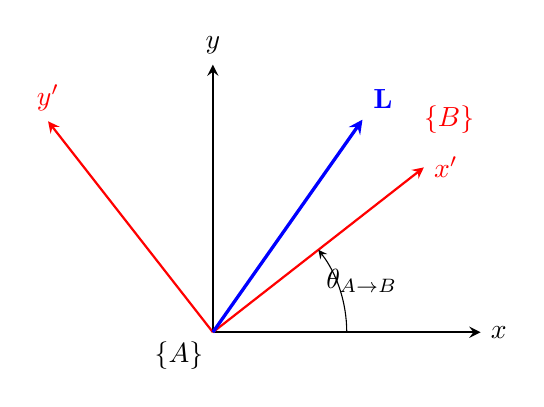
\begin{tikzpicture}[>=stealth,scale=1.0]
  % Frame {A}
  \draw[->,thick] (0,0) -- (3.4,0) node[right] {$x$};
  \draw[->,thick] (0,0) -- (0,3.4) node[above] {$y$};
  \node[below left] at (0,0) {$\{A\}$};
  % Frame {B}, rotated by theta
  \draw[->,thick,red,rotate=38] (0,0) -- (3.4,0) node[right] {$x'$};
  \draw[->,thick,red,rotate=38] (0,0) -- (0,3.4) node[above] {$y'$};
  \node[red] at (3.0,2.7) {$\{B\}$};
  % angle arc
  \draw[->] (1.7,0) arc (0:38:1.7);
  \node at (19:2.0) {$\theta_{A\to B}$};
  % vector L
  \draw[->,very thick,blue] (0,0) -- (1.9,2.7) node[above right] {$\vect{L}$};
\end{tikzpicture}
\caption{Frame $\{B\}$ is frame $\{A\}$ rotated by $\theta_{A\to B}$ about the $z$-axis; the vector $\vect{L}$ can be expressed in either frame.}
\label{fig:lec02-frames}
\end{figure}

The rotation matrix ${}^{A}_{B}\vect{R}$ maps a vector from $\{B\}$ to $\{A\}$:
\begin{align}
{}^{A}\vect{L} &= {}^{A}_{B}\vect{R}\,{}^{B}\vect{L} \\
&= {}^{A}_{B}\vect{R}(\theta_{A\to B})\,{}^{B}\vect{L}.
\end{align}
Adding the translation ${}^{A}\vect{p}_{B}$ (the origin of $\{B\}$ expressed in $\{A\}$, Fig.~\ref{fig:lec02-transl}) gives the full rigid-body transformation
\begin{align}
\{A\},\{B\} \;\Rightarrow\; \big\{\,{}^{A}_{B}\vect{R},\;{}^{A}\vect{p}_{B}\big\} \;\Rightarrow\;
{}^{A}_{B}\vect{T} = \begin{bmatrix} {}^{A}_{B}\vect{R} & {}^{A}\vect{p}_{B} \\ \vect{0}_{1\times3} & 1 \end{bmatrix}.
\end{align}

\begin{figure}[H]
\centering
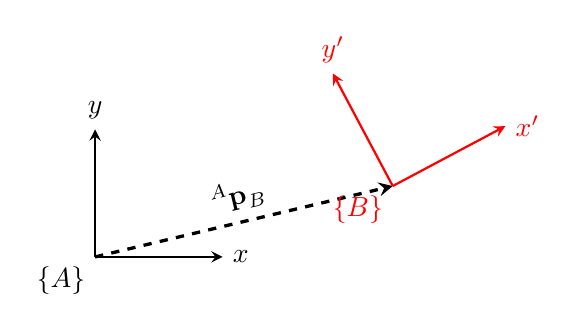
\begin{tikzpicture}[>=stealth,scale=0.9]
  % Frame A
  \draw[->,thick] (0,0) -- (1.8,0) node[right] {$x$};
  \draw[->,thick] (0,0) -- (0,1.8) node[above] {$y$};
  \node[below left] at (0,0) {$\{A\}$};
  % translation vector
  \draw[->,very thick,dashed] (0,0) -- (4.2,1.0) node[midway,above,sloped] {${}^{A}\vect{p}_{B}$};
  % Frame B
  \begin{scope}[shift={(4.2,1.0)},rotate=28]
    \draw[->,thick,red] (0,0) -- (1.8,0) node[right] {$x'$};
    \draw[->,thick,red] (0,0) -- (0,1.8) node[above] {$y'$};
    \node[red,below left] at (0,0) {$\{B\}$};
  \end{scope}
\end{tikzpicture}
\caption{A rigid-body transformation combines the rotation ${}^{A}_{B}\vect{R}$ with the translation ${}^{A}\vect{p}_{B}$.}
\label{fig:lec02-transl}
\end{figure}

% =====================================================================
\subsection{Defining rotation}

\paragraph{Euler angles.}
With roll $\theta$ (about $x$), pitch $r$ (about $y$), yaw $\psi$ (about $z$),
\begin{align}
\vect{R}(\theta) = \begin{bmatrix} 1 & 0 & 0 \\ 0 & \cos\theta & -\sin\theta \\ 0 & \sin\theta & \cos\theta \end{bmatrix},\;
\vect{R}(r) = \begin{bmatrix} \cos r & 0 & \sin r \\ 0 & 1 & 0 \\ -\sin r & 0 & \cos r \end{bmatrix},\;
\vect{R}(\psi) = \begin{bmatrix} \cos\psi & -\sin\psi & 0 \\ \sin\psi & \cos\psi & 0 \\ 0 & 0 & 1 \end{bmatrix},
\end{align}
and the yaw--pitch--roll composition is
\begin{align}
\vect{R} &= \vect{R}(\psi)\,\vect{R}(r)\,\vect{R}(\theta) \\
&= \begin{bmatrix} \cos\psi & -\sin\psi & 0 \\ \sin\psi & \cos\psi & 0 \\ 0 & 0 & 1 \end{bmatrix}
\begin{bmatrix} \cos r & 0 & \sin r \\ 0 & 1 & 0 \\ -\sin r & 0 & \cos r \end{bmatrix}
\begin{bmatrix} 1 & 0 & 0 \\ 0 & \cos\theta & -\sin\theta \\ 0 & \sin\theta & \cos\theta \end{bmatrix}.
\end{align}

\paragraph{Infinitesimal rotation and the skew-symmetric matrix.}
For small angles $\delta\theta,\delta r,\delta\psi\to 0$ each elementary rotation linearizes ($\cos\to1$, $\sin\to$ angle):
\begin{align}
\vect{R}(\delta\theta) = \begin{bmatrix} 1 & 0 & 0 \\ 0 & 1 & -\delta\theta \\ 0 & \delta\theta & 1 \end{bmatrix},\quad
\vect{R}(\delta r) = \begin{bmatrix} 1 & 0 & \delta r \\ 0 & 1 & 0 \\ -\delta r & 0 & 1 \end{bmatrix},\quad
\vect{R}(\delta\psi) = \begin{bmatrix} 1 & -\delta\psi & 0 \\ \delta\psi & 1 & 0 \\ 0 & 0 & 1 \end{bmatrix}.
\end{align}
Multiplying the last two and dropping all second-order products ($\delta r\,\delta\theta\approx0$ etc.),
\begin{align}
\vect{R}(\delta r)\vect{R}(\delta\theta)
&= \begin{bmatrix} 1 & 0 & \delta r \\ 0 & 1 & 0 \\ -\delta r & 0 & 1 \end{bmatrix}
\begin{bmatrix} 1 & 0 & 0 \\ 0 & 1 & -\delta\theta \\ 0 & \delta\theta & 1 \end{bmatrix} \\
&= \begin{bmatrix} 1 & 0 & \delta r \\ 0 & 1 & -\delta\theta \\ -\delta r & \delta\theta & 1 \end{bmatrix},
\end{align}
and then
\begin{align}
\vect{R} = \vect{R}(\delta\psi)\vect{R}(\delta r)\vect{R}(\delta\theta)
&= \begin{bmatrix} 1 & -\delta\psi & 0 \\ \delta\psi & 1 & 0 \\ 0 & 0 & 1 \end{bmatrix}
\begin{bmatrix} 1 & 0 & \delta r \\ 0 & 1 & -\delta\theta \\ -\delta r & \delta\theta & 1 \end{bmatrix} \notag\\
&= \begin{bmatrix} 1 & -\delta\psi & \delta r \\ \delta\psi & 1 & -\delta\theta \\ -\delta r & \delta\theta & 1 \end{bmatrix} \\
&= \vect{I} + \begin{bmatrix} 0 & -\delta\psi & \delta r \\ \delta\psi & 0 & -\delta\theta \\ -\delta r & \delta\theta & 0 \end{bmatrix} \\
&= \vect{I} + \skewsym{\vect{\theta}},
\end{align}
where the small-angle vector is $\vect{\theta} = [\delta\theta,\;\delta r,\;\delta\psi]\trans$. The matrix $\skewsym{\vect{\theta}}$ is skew-symmetric, $\skewsym{\vect{\theta}} = -\skewsym{\vect{\theta}}\trans$. This motivates writing a finite rotation as $\vect{R}(\vect{\theta}) \approx \vect{I} + \skewsym{\vect{\theta}} \approx \exp(\skewsym{\vect{\theta}})$, and defining $\Exp(\vect{\theta}) \triangleq \exp(\skewsym{\vect{\theta}})$. The question is then whether $\vect{R}(\vect{\theta}) = \Exp(\vect{\theta})$.

% =====================================================================
\subsection{Axis--angle and Rodrigues' formula}

Let $\vect{k}$ be the unit rotation axis and $\theta$ the rotation angle, with $\vect{\theta} = \theta\vect{k} = [\theta_1,\theta_2,\theta_3]\trans$, so
\begin{align}
\vect{k} = \begin{bmatrix} k_1 \\ k_2 \\ k_3 \end{bmatrix},\quad
\skewsym{\vect{k}} = \begin{bmatrix} 0 & -k_3 & k_2 \\ k_3 & 0 & -k_1 \\ -k_2 & k_1 & 0 \end{bmatrix},\quad
\skewsym{\vect{\theta}} = \begin{bmatrix} 0 & -\theta_3 & \theta_2 \\ \theta_3 & 0 & -\theta_1 \\ -\theta_2 & \theta_1 & 0 \end{bmatrix}.
\end{align}
The skew operator on a unit vector satisfies the cyclic power identities
\begin{align}
\skewsym{\vect{k}}^{2} &= \vect{k}\vect{k}\trans - \vect{I}_3, &
\skewsym{\vect{k}}^{3} &= -\skewsym{\vect{k}}, &
\skewsym{\vect{k}}^{4} &= -\skewsym{\vect{k}}^{2}, \\
\skewsym{\vect{k}}^{5} &= \skewsym{\vect{k}}, &
\skewsym{\vect{k}}^{6} &= \skewsym{\vect{k}}^{2}, &
\skewsym{\vect{k}}^{7} &= -\skewsym{\vect{k}}.
\end{align}
Substituting $\skewsym{\vect{\theta}} = \theta\skewsym{\vect{k}}$ into the exponential series term by term,
\begin{align}
\Exp(\vect{\theta}) = \exp(\theta\skewsym{\vect{k}})
&= \vect{I} + \theta\skewsym{\vect{k}} + \tfrac{\theta^2}{2!}\skewsym{\vect{k}}^2 + \tfrac{\theta^3}{3!}\skewsym{\vect{k}}^3 + \tfrac{\theta^4}{4!}\skewsym{\vect{k}}^4 \notag\\
&\quad + \tfrac{\theta^5}{5!}\skewsym{\vect{k}}^5 + \tfrac{\theta^6}{6!}\skewsym{\vect{k}}^6 + \tfrac{\theta^7}{7!}\skewsym{\vect{k}}^7 + \cdots \notag\\
&= \vect{I} + \theta\skewsym{\vect{k}} + \tfrac{\theta^2}{2!}\skewsym{\vect{k}}^2 - \tfrac{\theta^3}{3!}\skewsym{\vect{k}} - \tfrac{\theta^4}{4!}\skewsym{\vect{k}}^2 \notag\\
&\quad + \tfrac{\theta^5}{5!}\skewsym{\vect{k}} + \tfrac{\theta^6}{6!}\skewsym{\vect{k}}^2 - \tfrac{\theta^7}{7!}\skewsym{\vect{k}} + \cdots \notag\\
&= \vect{I} + \underbrace{\big(\theta - \tfrac{\theta^3}{3!} + \tfrac{\theta^5}{5!} - \tfrac{\theta^7}{7!} + \cdots\big)}_{\sin\theta}\skewsym{\vect{k}} \notag\\
&\quad + \underbrace{\big(\tfrac{\theta^2}{2!} - \tfrac{\theta^4}{4!} + \tfrac{\theta^6}{6!} - \cdots\big)}_{1-\cos\theta}\skewsym{\vect{k}}^2,
\end{align}
which gives \textbf{Rodrigues' rotation formula}
\begin{empheq}[box=\fbox]{align}
\vect{R}(\vect{\theta}) = \Exp(\vect{\theta}) = \exp(\theta\skewsym{\vect{k}})
= \vect{I} + \sin\theta\,\skewsym{\vect{k}} + (1-\cos\theta)\,\skewsym{\vect{k}}^2.
\end{empheq}
For a small angle $\delta\theta\to0$, $\vect{R}(\delta\vect{\theta}) \approx \vect{I} + \skewsym{\delta\vect{\theta}}$ (small-angle approximation).

\paragraph{Logarithmic map.}
The log map is the inverse of the exponential map:
\begin{align}
\log(\vect{R}) = \skewsym{\vect{\theta}}, \quad \Log(\vect{R}) = \vect{\theta}_{3\times1}, \qquad
\theta = \arccos\!\Big(\tfrac{\tr\vect{R} - 1}{2}\Big), \quad \skewsym{\vect{k}} = \frac{\vect{R} - \vect{R}\trans}{2\sin\theta}.
\end{align}

% =====================================================================
\subsection{SO(3) kinematics}

The two directions of the maps are: from the vector space $\Reals^3$ via the Lie algebra to the Lie group, $\vect{\theta} \to \skewsym{\vect{\theta}} \to \vect{R} = \Exp(\vect{\theta})$; and back, $\vect{R} \to \skewsym{\vect{\theta}} \to \vect{\theta} = \Log(\vect{R})$.

\paragraph{(1) Angular-velocity kinematics.} Differentiating the orthogonality constraint $\vect{R}\vect{R}\trans = \vect{I}_3$,
\begin{align}
\frac{\mathrm{d}}{\mathrm{d}t}(\vect{R}\vect{R}\trans) = \vect{0}
\;\Rightarrow\; \dot{\vect{R}}\vect{R}\trans + \vect{R}\dot{\vect{R}}\trans = \vect{0}
\;\Rightarrow\; \dot{\vect{R}}\vect{R}\trans = -\vect{R}\dot{\vect{R}}\trans = -(\dot{\vect{R}}\vect{R}\trans)\trans,
\end{align}
so $\dot{\vect{R}}\vect{R}\trans$ is skew-symmetric. Writing it as $\skewsym{\vect{\omega}}$ with $\skewsym{\vect{\omega}} = \begin{bmatrix} 0 & -\omega_3 & \omega_2 \\ \omega_3 & 0 & -\omega_1 \\ -\omega_2 & \omega_1 & 0 \end{bmatrix}$,
\begin{align}
\dot{\vect{R}}\vect{R}\trans = \skewsym{\vect{\omega}} \;\Rightarrow\; \dot{\vect{R}} = \skewsym{\vect{\omega}}\vect{R}.
\end{align}

\paragraph{(2) Equivalent limit form.} With $\vect{R}(t+\Delta t) = \vect{R}(t)\exp(\skewsym{\vect{\omega}}\Delta t)$,
\begin{align}
\dot{\vect{R}}(t) &= \lim_{\Delta t\to0}\frac{\vect{R}(t+\Delta t) - \vect{R}(t)}{\Delta t} \\
&= \lim_{\Delta t\to0}\frac{\vect{R}(t)\exp(\skewsym{\vect{\omega}}\Delta t) - \vect{R}(t)}{\Delta t} \\
&= \vect{R}(t)\lim_{\Delta t\to0}\frac{\exp(\skewsym{\vect{\omega}}\Delta t) - \vect{I}}{\Delta t} \\
&= \vect{R}(t)\skewsym{\vect{\omega}}.
\end{align}

\paragraph{(3) Integration.} With $\vect{R}_i = \exp(\skewsym{\vect{\omega}_i}\Delta t_i)$, composing increments gives
\begin{align}
\vect{R}_{1\to k} &= \vect{R}_k\vect{R}_{k-1}\cdots\vect{R}_2\vect{R}_1 \\
&= \exp(\skewsym{\vect{\omega}_k}\Delta t_k)\cdots\exp(\skewsym{\vect{\omega}_1}\Delta t_1).
\end{align}

\paragraph{(4) Interpolation.} For ${}^{G}_{t_1}\vect{R},{}^{G}_{t_2}\vect{R}$ and $t\in[t_1,t_2]$, define the relative rotation and its angle, and the interpolation ratio:
\begin{align}
{}^{t_1}_{t_2}\vect{R} &= {}^{G}_{t_1}\vect{R}\trans\,{}^{G}_{t_2}\vect{R}, \\
{}^{t_1}_{t_2}\vect{\theta} &= \Log({}^{t_1}_{t_2}\vect{R}) = \Log({}^{G}_{t_1}\vect{R}\trans\,{}^{G}_{t_2}\vect{R}), \\
\lambda &= \frac{t-t_1}{t_2-t_1}.
\end{align}
Then
\begin{align}
{}^{G}_{t}\vect{R} &= {}^{G}_{t_1}\vect{R}\,{}^{t_1}_{t}\vect{R} \\
&= {}^{G}_{t_1}\vect{R}\,\Exp\!\big(\lambda\,{}^{t_1}_{t_2}\vect{\theta}\big).
\end{align}

\paragraph{(5) Right Jacobian.} For a rotation $\vect{R}(\vect{\theta}) = \Exp(\vect{\theta})$, perturb the angle by $\delta\vect{\theta}\in\Reals^3$ and let $\delta\vect{\varphi}$ be the corresponding small rotation in $\mathfrak{so}(3)$:
\begin{align}
\vect{R}(\vect{\theta})\,\Exp(\delta\vect{\varphi}) = \vect{R}(\vect{\theta}+\delta\vect{\theta})
\;\Rightarrow\;
\Exp(\vect{\theta})\Exp(\delta\vect{\varphi}) = \Exp(\vect{\theta}+\delta\vect{\theta}).
\end{align}
Solving for $\delta\vect{\varphi}$,
\begin{align}
\Exp(\delta\vect{\varphi}) = \Exp(\vect{\theta})^{-1}\Exp(\vect{\theta}+\delta\vect{\theta})
\;\Rightarrow\;
\delta\vect{\varphi} = \Log\!\big(\Exp(\vect{\theta})^{-1}\Exp(\vect{\theta}+\delta\vect{\theta})\big),
\end{align}
and the \emph{right Jacobian} is the derivative of $\delta\vect{\varphi}$ with respect to $\delta\vect{\theta}$:
\begin{align}
\vect{J}_r(\vect{\theta}) \triangleq \frac{\partial\,\delta\vect{\varphi}}{\partial\,\delta\vect{\theta}}
= \lim_{\delta\vect{\theta}\to0}\frac{\Log\!\big(\Exp(\vect{\theta})^{-1}\Exp(\vect{\theta}+\delta\vect{\theta})\big)}{\delta\vect{\theta}}.
\end{align}
Equivalently, $\Exp(\vect{\theta}+\delta\vect{\theta}) = \Exp(\vect{\theta})\Exp\!\big(\vect{J}_r(\vect{\theta})\,\delta\vect{\theta}\big)$, and inverting,
\begin{align}
\Exp(\vect{\theta})\Exp(\delta\vect{\varphi}) = \Exp\!\big(\vect{\theta} + \vect{J}_r^{-1}(\vect{\theta})\,\delta\vect{\varphi}\big)
\;\Rightarrow\;
\Log\!\big(\Exp(\vect{\theta})\Exp(\delta\vect{\varphi})\big) = \vect{\theta} + \vect{J}_r^{-1}(\vect{\theta})\,\delta\vect{\varphi},
\end{align}
with the closed form
\begin{align}
\vect{J}_r(\vect{\theta}) = \vect{I} - \frac{1-\cos\norm{\vect{\theta}}}{\norm{\vect{\theta}}^{2}}\skewsym{\vect{\theta}} + \frac{\norm{\vect{\theta}}-\sin\norm{\vect{\theta}}}{\norm{\vect{\theta}}^{3}}\skewsym{\vect{\theta}}^{2}.
\end{align}

\paragraph{(6) Left Jacobian.} Applying the perturbation on the left instead defines the left Jacobian:
\begin{align}
\Exp(\vect{\theta}+\delta\vect{\theta}) = \Exp(\vect{\theta})\Exp\!\big(\vect{J}_r(\vect{\theta})\,\delta\vect{\theta}\big) = \Exp\!\big(\vect{J}_l(\vect{\theta})\,\delta\vect{\theta}\big)\Exp(\vect{\theta}).
\end{align}
Using the adjoint identity $\Exp(\vect{\theta})\Exp(\vect{x})\Exp(\vect{\theta})^{-1} = \Exp(\vect{R}(\vect{\theta})\vect{x})$ on the middle expression,
\begin{align}
\Exp(\vect{\theta})\Exp\!\big(\vect{J}_r\delta\vect{\theta}\big) = \Exp\!\big(\vect{R}(\vect{\theta})\vect{J}_r\delta\vect{\theta}\big)\Exp(\vect{\theta})
\;\Rightarrow\;
\vect{J}_l(\vect{\theta}) = \vect{R}(\vect{\theta})\,\vect{J}_r(\vect{\theta}).
\end{align}

\paragraph{(7) Sign symmetry.} From $\Exp(\vect{\theta}+\delta\vect{\theta}) = \Exp(\vect{\theta})\Exp(\vect{J}_r(\vect{\theta})\delta\vect{\theta})$, replacing $\vect{\theta}\to-\vect{\theta}$, $\delta\vect{\theta}\to-\delta\vect{\theta}$,
\begin{align}
\Exp(-\vect{\theta}-\delta\vect{\theta}) = \Exp\!\big(-\vect{J}_l(-\vect{\theta})\delta\vect{\theta}\big)\Exp(-\vect{\theta}) = \Exp\!\big(-\vect{J}_r(\vect{\theta})\delta\vect{\theta}\big)\Exp(-\vect{\theta})
\;\Rightarrow\;
\vect{J}_l(-\vect{\theta}) = \vect{J}_r(\vect{\theta}).
\end{align}

\paragraph{(8) Summary.} Collecting (5)--(7),
\begin{align}
\Exp(\vect{\theta}+\delta\vect{\theta}) = \Exp(\vect{\theta})\Exp\!\big(\vect{J}_r(\vect{\theta})\delta\vect{\theta}\big), \qquad
\vect{J}_l(\vect{\theta}) = \vect{R}(\vect{\theta})\vect{J}_r(\vect{\theta}), \qquad
\vect{J}_l(-\vect{\theta}) = \vect{J}_r(\vect{\theta}).
\end{align}

\paragraph{(9) Identity $\skewsym{\vect{R}\vect{\omega}} = \vect{R}\skewsym{\vect{\omega}}\vect{R}\trans$.} For any vector $\vect{v}$, using $\vect{R}(\vect{u}\times\vect{v}) = (\vect{R}\vect{u})\times(\vect{R}\vect{v})$ and $\vect{R}\trans\vect{R}=\vect{I}$,
\begin{align}
\skewsym{\vect{R}\vect{u}}(\vect{R}\vect{v})
&= \vect{R}\big(\skewsym{\vect{u}}\vect{v}\big) \\
&= \vect{R}\big(\skewsym{\vect{u}}\vect{R}\trans\vect{R}\vect{v}\big) \\
&= \vect{R}\skewsym{\vect{u}}\vect{R}\trans\,(\vect{R}\vect{v}).
\end{align}
Since this holds for all $\vect{R}\vect{v}$, we conclude $\skewsym{\vect{R}\vect{u}} = \vect{R}\skewsym{\vect{u}}\vect{R}\trans$.
\begin{quote}
\textbf{Homework.} Prove $\skewsym{\vect{R}\vect{\omega}} = \vect{R}\skewsym{\vect{\omega}}\vect{R}\trans$.
\end{quote}

\paragraph{(10) Identity $\Exp(\vect{R}\vect{\varphi}) = \vect{R}\,\Exp(\vect{\varphi})\,\vect{R}\trans$.} Using $\skewsym{\vect{R}\vect{\varphi}}^{k} = \vect{R}\skewsym{\vect{\varphi}}^{k}\vect{R}\trans$ (which follows from (9), since $\skewsym{\vect{R}\vect{\varphi}}^{2} = \vect{R}\skewsym{\vect{\varphi}}\vect{R}\trans\vect{R}\skewsym{\vect{\varphi}}\vect{R}\trans = \vect{R}\skewsym{\vect{\varphi}}^{2}\vect{R}\trans$, etc.),
\begin{align}
\Exp(\vect{R}\vect{\varphi})
&= \vect{I} + \skewsym{\vect{R}\vect{\varphi}} + \tfrac{1}{2!}\skewsym{\vect{R}\vect{\varphi}}^{2} + \tfrac{1}{3!}\skewsym{\vect{R}\vect{\varphi}}^{3} + \cdots \notag\\
&= \vect{R}\vect{R}\trans + \vect{R}\skewsym{\vect{\varphi}}\vect{R}\trans + \tfrac{1}{2!}\vect{R}\skewsym{\vect{\varphi}}^{2}\vect{R}\trans + \cdots \notag\\
&= \vect{R}\big(\vect{I} + \skewsym{\vect{\varphi}} + \tfrac{1}{2!}\skewsym{\vect{\varphi}}^{2} + \tfrac{1}{3!}\skewsym{\vect{\varphi}}^{3} + \cdots\big)\vect{R}\trans \\
&= \vect{R}\,\Exp(\vect{\varphi})\,\vect{R}\trans.
\end{align}
\begin{quote}
\textbf{Homework.} Prove $\Exp(\vect{R}\vect{\varphi}) = \vect{R}\,\Exp(\vect{\varphi})\,\vect{R}\trans$.
\end{quote}

\paragraph{Worked applications.}
\textbf{(11) Recovering ${}^{C}_{I}\vect{R}$ from vector pairs.} Given camera frame $\{C\}$ and IMU frame $\{I\}$ with ${}^{C}\vect{v}_1 = {}^{C}_{I}\vect{R}\,{}^{I}\vect{v}_1$ and ${}^{C}\vect{v}_2 = {}^{C}_{I}\vect{R}\,{}^{I}\vect{v}_2$, the trick is to stack three independent directions (the third from the cross product) into an invertible matrix:
\begin{align}
\big[\,{}^{C}\vect{v}_1 \;\; {}^{C}\vect{v}_2 \;\; {}^{C}\vect{v}_1\times{}^{C}\vect{v}_2\,\big]
= {}^{C}_{I}\vect{R}\,\big[\,{}^{I}\vect{v}_1 \;\; {}^{I}\vect{v}_2 \;\; {}^{I}\vect{v}_1\times{}^{I}\vect{v}_2\,\big].
\end{align}
\textbf{(12)} Given instead relative rotations ${}^{C_1}_{C_2}\vect{R} = {}^{C}_{I}\vect{R}\,{}^{I_1}_{I_2}\vect{R}\,{}^{C}_{I}\vect{R}\trans$, recover ${}^{C}_{I}\vect{R}$ from two such pairs.
\begin{quote}
\textbf{(13) Discussion.} For (11)/(12): What is the minimum number of data pairs needed? What requirements must the pairs satisfy? What if more than the minimum is available?
\end{quote}
\textbf{(14) Averaging noisy rotations.} Given $n$ measurements $\vect{R}_{m_i} = \vect{R}\,\exp(\skewsym{\vect{n}_i})$ with $\vect{n}_i\sim\mathcal{N}(\vect{0}_{3\times1},\vect{P}_i)$, estimate $\vect{R}$ and its covariance.

% =====================================================================
\subsection{Groups: SO(3) and SE(3)}

\paragraph{SO(3) --- special orthogonal group.}
\begin{align}
SO(3) = \big\{\vect{R}\in\Reals^{3\times3} \;\big|\; \vect{R}\trans\vect{R} = \vect{I}_3,\;\det(\vect{R}) = 1\big\}.
\end{align}
It satisfies the four group axioms: \emph{closure} ($\vect{R}_1\vect{R}_2\in SO(3)$), \emph{identity} ($\vect{I}_3\in SO(3)$), \emph{inverse} ($\vect{R}^{-1} = \vect{R}\trans\in SO(3)$), and \emph{associativity} ($(\vect{R}_1\vect{R}_2)\vect{R}_3 = \vect{R}_1(\vect{R}_2\vect{R}_3)$).

\paragraph{SE(3) --- special Euclidean group.}
\begin{align}
SE(3) = \left\{\vect{T} = \begin{bmatrix} \vect{R} & \vect{p} \\ \vect{0}_{1\times3} & 1 \end{bmatrix} \;\middle|\; \vect{R}\in SO(3),\;\vect{p}\in\Reals^{3}\right\}.
\end{align}
The four axioms: \emph{closure}
\begin{align}
\vect{T}_1\vect{T}_2 &= \begin{bmatrix}\vect{R}_1 & \vect{p}_1\\\vect{0} & 1\end{bmatrix}\begin{bmatrix}\vect{R}_2 & \vect{p}_2\\\vect{0} & 1\end{bmatrix} \\
&= \begin{bmatrix}\vect{R}_1\vect{R}_2 & \vect{R}_1\vect{p}_2+\vect{p}_1\\\vect{0} & 1\end{bmatrix} \in SE(3),
\end{align}
\emph{identity} $\begin{bmatrix}\vect{I}_3 & \vect{0}_{3\times1}\\\vect{0}_{1\times3} & 1\end{bmatrix}$, \emph{inverse}
\begin{align}
\begin{bmatrix} \vect{R} & \vect{p} \\ \vect{0} & 1 \end{bmatrix}^{-1} = \begin{bmatrix} \vect{R}\trans & -\vect{R}\trans\vect{p} \\ \vect{0} & 1 \end{bmatrix} \in SE(3),
\end{align}
and \emph{associativity} $(\vect{T}_1\vect{T}_2)\vect{T}_3 = \vect{T}_1(\vect{T}_2\vect{T}_3)$.

\paragraph{Matrix Lie groups.}
A \emph{group} is a set with an operation satisfying closure, associativity, identity, and invertibility. A \emph{Lie group} is a group that is also a smooth (differentiable) manifold whose group operation is smooth. A \emph{matrix Lie group} has matrices as its elements. The maps between the vector space, the Lie algebra, and the Lie group are
\begin{align}
\Reals^{m} \xrightarrow{\;\wedge\;(\text{wedge})\;} \mathfrak{so}(n) \xrightarrow{\;\exp\;} SO(n), \qquad
SO(n) \xrightarrow{\;\log\;} \mathfrak{so}(n) \xrightarrow{\;\vee\;(\text{vee})\;} \Reals^{m},
\end{align}
and for short we write $\vect{X} = \Exp(\vect{x}) = \exp(\vect{x}^{\wedge})$ and $\vect{x} = \Log(\vect{X}) = \log(\vect{X})^{\vee}$. For $SO(3)$ specifically, $\vect{\theta}\in\Reals^3 \to \skewsym{\vect{\theta}} = \vect{\theta}^{\wedge} \to \vect{R} = \exp(\vect{\theta}^{\wedge})$, and $\vect{R}\in SO(3) \to \skewsym{\vect{\theta}} = \log(\vect{R}) \to \vect{\theta} = \log(\vect{R})^{\vee}$.

\paragraph{Why this (manifold) machinery?}
It \emph{simplifies} estimation: the core idea is to use a smooth manifold to model parameters that are awkward in plain vector space, which makes optimization, interpolation, integration, and differentiation easier or even possible (Fig.~\ref{fig:lec02-manifold}). For example, a raw angle $\theta\in[-\pi,\pi]$ has a wrap-around cut; the circle/sphere is smooth, and the tangent line at a point models the small change / error state used in optimization.

\begin{figure}[H]
\centering
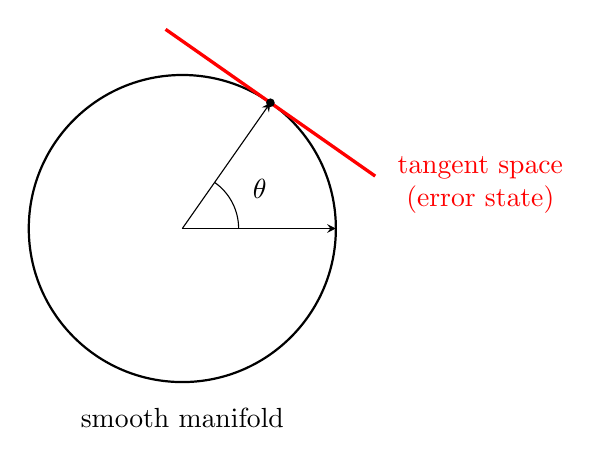
\begin{tikzpicture}[>=stealth,scale=1.3]
  % manifold (circle)
  \draw[thick] (0,0) circle (1.5);
  % radii and angle
  \draw[->] (0,0) -- (0:1.5);
  \draw[->] (0,0) -- (55:1.5);
  \draw (0:0.55) arc (0:55:0.55);
  \node at (27:0.85) {$\theta$};
  % tangent at point P=(55:1.5)
  \coordinate (P) at (55:1.5);
  \draw[red,very thick] ($(P)+(145:1.25)$) -- ($(P)+(-35:1.25)$);
  \fill (P) circle (1.2pt);
  \node[red,align=center,anchor=west] at ($(P)+(-35:1.4)$) {tangent space\\(error state)};
  \node at (0,-1.85) {smooth manifold};
\end{tikzpicture}
\caption{A smooth manifold (here a circle/sphere) avoids the wrap-around of a raw angle; the red tangent line is the local vector space used to model derivatives and error states for optimization.}
\label{fig:lec02-manifold}
\end{figure}

For $SO(3)$ the left Jacobian also appears directly in the exponential expansion:
\begin{align}
\vect{R}(\vect{\theta}) &= \Exp(\vect{\theta}) \\
&= \vect{I}_3 + \skewsym{\vect{\theta}}\vect{J}_l(\vect{\theta}) = \vect{I}_3 + \vect{\theta}^{\wedge}\vect{J}_l(\vect{\theta}), \\
\vect{J}_l(\vect{\theta}) &= \sum_{n=0}^{\infty}\frac{1}{(n+1)!}(\vect{\theta}^{\wedge})^{n}.
\end{align}

% =====================================================================
\subsection{SE(3)}

\paragraph{Exp / Log.} The SE(3) tangent vector uses $\vect{\rho}$ for its translation component, $\vect{\xi} = \begin{bmatrix}\vect{\theta}\\\vect{\rho}\end{bmatrix}\in\Reals^6$, which is \emph{distinct} from the group translation $\vect{p}$ in $\vect{T} = \begin{bmatrix}\vect{R} & \vect{p}\\ \vect{0} & 1\end{bmatrix}$; the two are related by $\vect{p} = \vect{J}_l(\vect{\theta})\vect{\rho}$. With the $4\times4$ algebra element $\vect{\xi}^{\wedge} = \begin{bmatrix}\skewsym{\vect{\theta}} & \vect{\rho}\\ \vect{0}_{1\times3} & 0\end{bmatrix}$,
\begin{align}
\vect{T} = \Exp(\vect{\xi}) &= \exp\!\begin{bmatrix}\skewsym{\vect{\theta}} & \vect{\rho}\\ \vect{0} & 0\end{bmatrix} \\
&= \begin{bmatrix} \exp(\skewsym{\vect{\theta}}) & \vect{J}_l(\vect{\theta})\,\vect{\rho} \\ \vect{0}_{1\times3} & 1 \end{bmatrix} \\
&= \begin{bmatrix} \vect{R} & \vect{p} \\ \vect{0} & 1 \end{bmatrix}, \qquad \vect{p} = \vect{J}_l(\vect{\theta})\,\vect{\rho},
\end{align}
and inverting,
\begin{align}
\vect{\xi} = \Log(\vect{T})^{\vee}, \qquad
\log(\vect{T}) &= \log\begin{bmatrix}\vect{R} & \vect{p}\\ \vect{0} & 1\end{bmatrix} \\
&= \begin{bmatrix}\log(\vect{R}) & \vect{J}_l^{-1}(\vect{\theta})\vect{p}\\ \vect{0} & 0\end{bmatrix}
\;\Rightarrow\;
\vect{\xi} = \begin{bmatrix}\vect{\theta}\\ \vect{J}_l^{-1}(\vect{\theta})\vect{p}\end{bmatrix} = \begin{bmatrix}\vect{\theta}\\ \vect{\rho}\end{bmatrix}.
\end{align}
\begin{quote}
\textbf{Discussion.} Prove $\exp\!\Big(\begin{bmatrix}\skewsym{\vect{\theta}} & \vect{\rho}\\ \vect{0} & 0\end{bmatrix}\Big) = \begin{bmatrix}\vect{R} & \vect{J}_l(\vect{\theta})\vect{\rho}\\ \vect{0} & 1\end{bmatrix}$.
\end{quote}

\paragraph{Left/right Jacobians.} With $\Exp(\vect{\xi}+\delta\vect{\xi}) = \Exp(\vect{\xi})\Exp(\vect{J}_R(\vect{\xi})\delta\vect{\xi}) = \Exp(\vect{J}_L(\vect{\xi})\delta\vect{\xi})\Exp(\vect{\xi})$,
\begin{align}
\vect{J}_R(\vect{\xi}) = \begin{bmatrix} \vect{J}_R(\vect{\theta}) & \vect{0} \\ \vect{Q}_R(\vect{\xi}) & \vect{J}_R(\vect{\theta}) \end{bmatrix}_{6\times6}, \quad
\vect{J}_L(\vect{\xi}) = \begin{bmatrix} \vect{J}_L(\vect{\theta}) & \vect{0} \\ \vect{Q}_L(\vect{\xi}) & \vect{J}_L(\vect{\theta}) \end{bmatrix}_{6\times6},
\end{align}
and to first order, with $\vect{\xi}^{\curlywedge} = \begin{bmatrix}\skewsym{\vect{\theta}} & \vect{0}\\ \skewsym{\vect{\rho}} & \skewsym{\vect{\theta}}\end{bmatrix}_{6\times6}$,
\begin{align}
\vect{J}_L(\vect{\xi}) \approx \vect{I}_6 + \tfrac{1}{2}\vect{\xi}^{\curlywedge}, \qquad
\vect{J}_R(\vect{\xi}) \approx \vect{I}_6 - \tfrac{1}{2}\vect{\xi}^{\curlywedge}.
\end{align}
\begin{quote}
\textbf{Homework.} Find $\vect{Q}_L$ (and $\vect{Q}_R$).
\end{quote}

\paragraph{Error states: SE(3) vs SO(3)\,$+\,\Reals^3$.} Perturb $\vect{T}$ on the right by the SE(3) tangent $\delta\vect{\xi} = [\delta\vect{\theta}\trans,\;\delta\vect{\rho}\trans]\trans$. Expanding with $\vect{J}_l(\delta\vect{\theta})\approx\vect{I}+\tfrac12\skewsym{\delta\vect{\theta}}$ and $\delta\vect{R} = \Exp(\delta\vect{\theta})$,
\begin{align}
\vect{T}\,\delta\vect{T}
&= \begin{bmatrix}\vect{R}&\vect{p}\\\vect{0}&1\end{bmatrix}\begin{bmatrix}\Exp(\delta\vect{\theta}) & \vect{J}_l(\delta\vect{\theta})\delta\vect{\rho}\\\vect{0}&1\end{bmatrix} \\
&= \begin{bmatrix}\vect{R}&\vect{p}\\\vect{0}&1\end{bmatrix}\begin{bmatrix}\delta\vect{R} & (\vect{I}+\tfrac12\skewsym{\delta\vect{\theta}})\delta\vect{\rho}\\\vect{0}&1\end{bmatrix} \\
&\approx \begin{bmatrix}\vect{R}&\vect{p}\\\vect{0}&1\end{bmatrix}\begin{bmatrix}\delta\vect{R} & \delta\vect{\rho}\\\vect{0}&1\end{bmatrix} \\
&= \begin{bmatrix}\vect{R}\delta\vect{R} & \vect{R}\delta\vect{\rho}+\vect{p}\\ \vect{0}&1\end{bmatrix}.
\end{align}
If instead we treat the pose as $SO(3)+\Reals^3$ (rotation and translation perturbed separately, $\vect{p}\to\vect{p}+\delta\vect{p}$),
\begin{align}
\vect{T} &= \begin{bmatrix}\vect{R}\delta\vect{R} & \vect{p}+\delta\vect{p}\\\vect{0}&1\end{bmatrix} \\
&= \begin{bmatrix}\vect{R}\delta\vect{R} & \vect{p}+\vect{R}\vect{R}\trans\delta\vect{p}\\\vect{0}&1\end{bmatrix} \\
&= \begin{bmatrix}\vect{R}&\vect{p}\\\vect{0}&1\end{bmatrix}\begin{bmatrix}\delta\vect{R} & \vect{R}\trans\delta\vect{p}\\\vect{0}&1\end{bmatrix}.
\end{align}
Comparing the two conventions gives the relation between the error states (SE(3) tangent translation $\delta\vect{\rho}$ vs.\ naive position error $\delta\vect{p}$),
\begin{align}
\begin{bmatrix}\vect{R}&\vect{p}\\\vect{0}&1\end{bmatrix}\begin{bmatrix}\delta\vect{R}&\delta\vect{p}\\\vect{0}&1\end{bmatrix}_{SO(3)+\Reals^3}
= \begin{bmatrix}\vect{R}&\vect{p}\\\vect{0}&1\end{bmatrix}\begin{bmatrix}\delta\vect{R}&\delta\vect{\rho}\\\vect{0}&1\end{bmatrix}_{SE(3)}
\;\Rightarrow\;
\begin{cases} \delta\vect{\rho} = \vect{R}\trans\delta\vect{p} \\ \delta\vect{R}_{SE(3)} = \delta\vect{R} \end{cases}.
\end{align}

\paragraph{Adjoint.} The adjoint transfers algebra elements across the group:
\begin{align}
SO(3):\;\; \vect{R}\,\Exp(\vect{\varphi})\,\vect{R}\trans = \Exp(\vect{R}\vect{\varphi}) \;\Leftrightarrow\; \Ad_{\vect{R}} = \vect{R}, \qquad
SE(3):\;\; \vect{T}\,\Exp(\vect{\xi})\,\vect{T}^{-1} = \Exp(\Ad_{\vect{T}}\vect{\xi}),
\end{align}
with $\Ad_{\vect{T}} = \begin{bmatrix}\vect{R} & \vect{0}\\ \skewsym{\vect{p}}\vect{R} & \vect{R}\end{bmatrix}_{6\times6}$. The adjoint is itself a Lie group, with $\Ad_{\vect{T}} = \exp(\vect{\xi}^{\curlywedge})$ and $\log(\Ad_{\vect{T}})^{\vee} = \vect{\xi}$.
\begin{quote}
\textbf{Homework.} Prove $\vect{T}\,\Exp(\vect{\xi})\,\vect{T}^{-1} = \Exp(\Ad_{\vect{T}}\vect{\xi})$.
\end{quote}

\subsubsection*{More operations}
\paragraph{(1) Interpolation.} For ${}^{G}_{t_1}\vect{T},{}^{G}_{t_2}\vect{T}$, $t\in[t_1,t_2]$, $\lambda = \tfrac{t-t_1}{t_2-t_1}$: in $SE(3)$, with ${}^{t_1}_{t_2}\vect{\xi} = \Log({}^{G}_{t_1}\vect{T}^{-1}\,{}^{G}_{t_2}\vect{T})$,
\begin{align}
{}^{G}_{t}\vect{T} = {}^{G}_{t_1}\vect{T}\,\Exp\!\big(\lambda\,{}^{t_1}_{t_2}\vect{\xi}\big);
\end{align}
in $SO(3)+\Reals^3$, the rotation interpolates on the manifold and the position linearly:
\begin{align}
{}^{G}_{t}\vect{R} = {}^{G}_{t_1}\vect{R}\,\Exp\!\big(\lambda\Log({}^{G}_{t_1}\vect{R}\trans\,{}^{G}_{t_2}\vect{R})\big), \qquad
{}^{G}\vect{p}_{t} = {}^{G}\vect{p}_{t_1} + \lambda({}^{G}\vect{p}_{t_2} - {}^{G}\vect{p}_{t_1}).
\end{align}

\paragraph{(2) Time derivative.} For $SE(3)$, with $\vect{T} = \vect{T}\,\Exp\!\big([\delta\vect{\theta};\delta\vect{\rho}]^{\wedge}\big)$ and body velocity, expand the limit using $\exp(\skewsym{\delta\vect{\theta}})-\vect{I}_3\approx\skewsym{\delta\vect{\theta}}$ and $\vect{J}_l(\delta\vect{\theta})\approx\vect{I}+\tfrac12\skewsym{\delta\vect{\theta}}$:
\begin{align}
\frac{\mathrm{d}\vect{T}}{\mathrm{d}t}
&= \lim_{\delta t\to0}\frac{\vect{T}(t+\delta t)-\vect{T}(t)}{\delta t} \\
&= \lim_{\delta t\to0}\frac{1}{\delta t}\left(\begin{bmatrix}\vect{R}&\vect{p}\\\vect{0}&1\end{bmatrix}\begin{bmatrix}\exp(\skewsym{\delta\vect{\theta}}) & \vect{J}_l(\delta\vect{\theta})\delta\vect{\rho}\\\vect{0}&1\end{bmatrix} - \begin{bmatrix}\vect{R}&\vect{p}\\\vect{0}&1\end{bmatrix}\right) \\
&= \lim_{\delta t\to0}\frac{1}{\delta t}\begin{bmatrix}\vect{R}&\vect{p}\\\vect{0}&1\end{bmatrix}\begin{bmatrix}\exp(\skewsym{\delta\vect{\theta}})-\vect{I}_3 & \vect{J}_l(\delta\vect{\theta})\delta\vect{\rho}\\\vect{0}&0\end{bmatrix} \\
&= \lim_{\delta t\to0}\frac{1}{\delta t}\begin{bmatrix}\vect{R}&\vect{p}\\\vect{0}&1\end{bmatrix}\begin{bmatrix}\skewsym{\delta\vect{\theta}} & \delta\vect{\rho}\\\vect{0}&0\end{bmatrix} \\
&= \begin{bmatrix}\vect{R}&\vect{p}\\\vect{0}&1\end{bmatrix}\begin{bmatrix}\skewsym{\vect{\omega}} & \vect{v}\\\vect{0}&0\end{bmatrix} \\
&= \begin{bmatrix}\vect{R}\skewsym{\vect{\omega}} & \vect{R}\vect{v}\\\vect{0}&0\end{bmatrix},
\end{align}
where $\vect{v}$ is the body velocity. For $SO(3)+\Reals^3$ the same computation with
\begin{align}
\vect{T} = \begin{bmatrix}\vect{R}\exp(\skewsym{\delta\vect{\theta}}) & \vect{p}+\delta\vect{p}\\\vect{0}&1\end{bmatrix}
\end{align}
gives
\begin{align}
\frac{\mathrm{d}\vect{T}}{\mathrm{d}t} = \begin{bmatrix}\vect{R}\skewsym{\vect{\omega}} & {}^{G}\vect{v}\\\vect{0}&0\end{bmatrix},
\end{align}
with ${}^{G}\vect{v}$ the global velocity.

\paragraph{(3) Calibration.} For IMU frame $\{I\}$ and camera frame $\{C\}$,
\begin{align}
{}^{C_1}_{C_2}\vect{T} = {}^{C}_{I}\vect{T}\,{}^{I_1}_{I_2}\vect{T}\,{}^{C}_{I}\vect{T}^{-1}, \qquad
\Exp({}^{C_1}_{C_2}\vect{\xi}) = \Exp\!\big(\Ad_{({}^{C}_{I}\vect{T})}\,{}^{I_1}_{I_2}\vect{\xi}\big)\;\Rightarrow\;{}^{C_1}_{C_2}\vect{\xi} = \Ad_{({}^{C}_{I}\vect{T})}\,{}^{I_1}_{I_2}\vect{\xi}.
\end{align}
\begin{quote}
\textbf{Homework.} Compute the Jacobians $\partial\,{}^{C_1}_{C_2}\vect{\xi}/\partial\,{}^{I_1}_{I_2}\vect{\xi}$ and $\partial\,{}^{C_1}_{C_2}\vect{\xi}/\partial\,{}^{C}_{I}\vect{\xi}$ (and the corresponding $SO(3)+\Reals^3$ versions).
\end{quote}

% =====================================================================
\subsection{SE\texorpdfstring{$_2$}{2}(3)}
Augmenting the pose with a velocity column gives the $5\times5$ group element
\begin{align}
\vect{\Upsilon} = \begin{bmatrix} \vect{R} & \vect{p} & \vect{v} \\ \vect{0}_{1\times3} & 1 & 0 \\ \vect{0}_{1\times3} & 0 & 1 \end{bmatrix}, \qquad
\vect{\xi} = \begin{bmatrix}\vect{\theta}\\\vect{\rho}\\\vect{\nu}\end{bmatrix} \to \vect{\xi}^{\wedge} = \begin{bmatrix}\skewsym{\vect{\theta}} & \vect{\rho} & \vect{\nu} \\ \vect{0} & 0 & 0 \\ \vect{0} & 0 & 0\end{bmatrix}_{5\times5},
\end{align}
where (as in SE(3)) the tangent components $\vect{\rho},\vect{\nu}$ are distinct from the group position/velocity $\vect{p} = \vect{J}_l(\vect{\theta})\vect{\rho}$, $\vect{v} = \vect{J}_l(\vect{\theta})\vect{\nu}$. The exponential, logarithm, and adjoint follow the same pattern as $SE(3)$:
\begin{align}
\Exp(\vect{\xi}) &= \begin{bmatrix} \vect{R} & \vect{J}_l(\vect{\theta})\vect{\rho} & \vect{J}_l(\vect{\theta})\vect{\nu} \\ \vect{0} & 1 & 0 \\ \vect{0} & 0 & 1\end{bmatrix} = \begin{bmatrix}\vect{R} & \vect{p} & \vect{v}\\ \vect{0} & 1 & 0\\ \vect{0} & 0 & 1\end{bmatrix}, \\
\Log(\vect{\Upsilon})^{\vee} &= \begin{bmatrix}\vect{\theta}\\ \vect{J}_l^{-1}(\vect{\theta})\vect{p}\\ \vect{J}_l^{-1}(\vect{\theta})\vect{v}\end{bmatrix}, \qquad
\Ad_{\vect{\Upsilon}} = \begin{bmatrix}\vect{R} & \vect{0} & \vect{0}\\ \skewsym{\vect{p}}\vect{R} & \vect{R} & \vect{0}\\ \skewsym{\vect{v}}\vect{R} & \vect{0} & \vect{R}\end{bmatrix}.
\end{align}

% =====================================================================
\subsection{Quaternions}
Quaternions are presented last because $SO(3)$, $SE(3)$, and the Lie-group view already cover most needs. There are two main conventions --- \emph{Hamilton} (right-handed) and \emph{JPL} (left-handed); we use the \textbf{Hamilton} convention. For a thorough treatment see Sol\`a~\cite{Sola2017Quaternion} (Hamilton) and Trawny \& Roumeliotis~\cite{Trawny2005Quaternion} (JPL).

A quaternion and its imaginary units satisfy
\begin{align}
Q = q_w + q_x i + q_y j + q_z k, \qquad i^2 = j^2 = k^2 = ijk = -1, \quad ij = k,\; jk = i,\; ki = j,
\end{align}
written as the $4\times1$ vector $\bar{q} = [q_w,\;q_x,\;q_y,\;q_z]\trans = [q_w,\;\vect{q}_v\trans]\trans$.

\paragraph{Product.} The quaternion product is bilinear and can be written with left/right matrices:
\begin{align}
\bar{p}\otimes\bar{q} &= \mathcal{L}(\bar{p})\,\bar{q} = \mathcal{R}(\bar{q})\,\bar{p}, \\
\mathcal{L}(\bar{p}) &= p_w\vect{I}_4 + \begin{bmatrix} 0 & -\vect{p}_v\trans \\ \vect{p}_v & \skewsym{\vect{p}_v} \end{bmatrix}, \\
\mathcal{R}(\bar{q}) &= q_w\vect{I}_4 + \begin{bmatrix} 0 & -\vect{q}_v\trans \\ \vect{q}_v & -\skewsym{\vect{q}_v} \end{bmatrix}.
\end{align}

\paragraph{Identity, unit quaternion, inverse.} The identity is $\bar{q} = [1,\;\vect{0}_{3\times1}\trans]\trans$. A rotation by angle $\theta$ about unit axis $\vect{k}$ is the unit quaternion
\begin{align}
\bar{q} = \begin{bmatrix}\cos\tfrac{\theta}{2}\\ \sin\tfrac{\theta}{2}\,\vect{k}\end{bmatrix}, \qquad
\bar{q}^{-1} = \begin{bmatrix}\cos\tfrac{\theta}{2}\\ -\sin\tfrac{\theta}{2}\,\vect{k}\end{bmatrix}, \qquad
\vect{R}_{12} = \vect{R}_1\vect{R}_2 \;\leftrightarrow\; \bar{q}_{12} = \bar{q}_1\otimes\bar{q}_2.
\end{align}

\paragraph{Why $\theta/2$? --- rotating a vector.} With global frame $\{G\}$ and IMU frame $\{I\}$, rotate ${}^{I}\vect{p}$ via the sandwich product and convert to matrices with $\bar p \otimes \bar q = \mathcal{R}(\bar q)\bar p$ and $\bar p\otimes \bar q=\mathcal{L}(\bar p)\bar q$:
\begin{align}
\begin{bmatrix}0\\ {}^{G}\vect{p}\end{bmatrix}
&= {}^{G}_{I}\bar{q}\otimes\begin{bmatrix}0\\ {}^{I}\vect{p}\end{bmatrix}\otimes{}^{G}_{I}\bar{q}^{-1} \\
&= \mathcal{R}({}^{G}_{I}\bar{q}^{-1})\,\mathcal{L}({}^{G}_{I}\bar{q})\begin{bmatrix}0\\ {}^{I}\vect{p}\end{bmatrix}.
\end{align}
Writing $\bar q = [q_w,\vect{q}_v\trans]\trans$ and multiplying the two matrices,
\begin{align}
\mathcal{R}(\bar{q}^{-1})\mathcal{L}(\bar{q})
&= \left(q_w\vect{I}_4 + \begin{bmatrix}0 & \vect{q}_v\trans\\ -\vect{q}_v & \skewsym{\vect{q}_v}\end{bmatrix}\right)\!\left(q_w\vect{I}_4 + \begin{bmatrix}0 & -\vect{q}_v\trans\\ \vect{q}_v & \skewsym{\vect{q}_v}\end{bmatrix}\right) \notag\\
&= q_w^2\vect{I}_4 + 2q_w\begin{bmatrix}0 & \vect{0}\\ \vect{0} & \skewsym{\vect{q}_v}\end{bmatrix} + \begin{bmatrix}\vect{q}_v\trans\vect{q}_v & \vect{0}\\ \vect{0} & -\vect{q}_v\vect{q}_v\trans + \skewsym{\vect{q}_v}^2\end{bmatrix},
\end{align}
whose lower-right $3\times3$ block (acting on ${}^{I}\vect{p}$) gives
\begin{align}
{}^{G}\vect{p} = \big(q_w^2\vect{I}_3 + 2q_w\skewsym{\vect{q}_v} + \vect{q}_v\vect{q}_v\trans + \skewsym{\vect{q}_v}^2\big){}^{I}\vect{p}.
\end{align}
Using $\skewsym{\vect{q}_v}^2 = \vect{q}_v\vect{q}_v\trans - (\vect{q}_v\trans\vect{q}_v)\vect{I}_3$ and the unit-norm condition $q_w^2 + \vect{q}_v\trans\vect{q}_v = 1$,
\begin{align}
q_w^2\vect{I}_3 + \vect{q}_v\vect{q}_v\trans + \skewsym{\vect{q}_v}^2
&= q_w^2\vect{I}_3 + (\vect{q}_v\trans\vect{q}_v)\vect{I}_3 + 2\skewsym{\vect{q}_v}^2 \\
&= \vect{I}_3 + 2\skewsym{\vect{q}_v}^2,
\end{align}
so
\begin{align}
{}^{G}\vect{p} = \big(\vect{I}_3 + 2q_w\skewsym{\vect{q}_v} + 2\skewsym{\vect{q}_v}^2\big){}^{I}\vect{p}.
\end{align}
Finally substitute $q_w = \cos\tfrac{\theta}{2}$, $\vect{q}_v = \sin\tfrac{\theta}{2}\vect{k}$, so $2q_w\skewsym{\vect{q}_v} = 2\cos\tfrac{\theta}{2}\sin\tfrac{\theta}{2}\skewsym{\vect{k}} = \sin\theta\,\skewsym{\vect{k}}$ and $2\skewsym{\vect{q}_v}^2 = 2\sin^2\tfrac{\theta}{2}\skewsym{\vect{k}}^2 = (1-\cos\theta)\skewsym{\vect{k}}^2$:
\begin{align}
{}^{G}\vect{p} &= \big(\vect{I}_3 + \sin\theta\,\skewsym{\vect{k}} + (1-\cos\theta)\skewsym{\vect{k}}^2\big){}^{I}\vect{p} \\
&= {}^{G}_{I}\vect{R}\,{}^{I}\vect{p} \\
&= \Exp(\theta\vect{k})\,{}^{I}\vect{p},
\end{align}
recovering Rodrigues' formula --- which is why the half-angle $\theta/2$ appears.

\paragraph{Derivative.} With $\delta\vect{\theta} = \delta\theta\,\vect{k}$ and small-angle $\delta\bar{q} = [\cos\tfrac{\delta\theta}{2},\;\sin\tfrac{\delta\theta}{2}\vect{k}\trans]\trans \approx [1,\;\tfrac12\delta\vect{\theta}\trans]\trans$,
\begin{align}
{}^{G}_{t}\dot{\bar{q}}
&= \lim_{\Delta t\to0}\frac{{}^{G}_{t+\Delta t}\bar{q} - {}^{G}_{t}\bar{q}}{\Delta t} \\
&= \lim_{\Delta t\to0}\frac{{}^{G}_{t}\bar{q}\otimes\begin{bmatrix}\cos\tfrac{\delta\theta}{2}\\ \sin\tfrac{\delta\theta}{2}\vect{k}\end{bmatrix} - {}^{G}_{t}\bar{q}\otimes\begin{bmatrix}1\\ \vect{0}\end{bmatrix}}{\Delta t} \\
&= \lim_{\Delta t\to0}\frac{{}^{G}_{t}\bar{q}\otimes\begin{bmatrix}0\\ \tfrac12\delta\vect{\theta}\end{bmatrix}}{\Delta t} \\
&= {}^{G}_{t}\bar{q}\otimes\begin{bmatrix}0\\ \tfrac12\vect{\omega}\end{bmatrix} \\
&= \tfrac12\,\mathcal{R}\!\left(\begin{bmatrix}0\\ \vect{\omega}\end{bmatrix}\right){}^{G}_{t}\bar{q} \\
&= \tfrac12\begin{bmatrix}0 & -\vect{\omega}\trans\\ \vect{\omega} & -\skewsym{\vect{\omega}}\end{bmatrix}{}^{G}_{t}\bar{q} \\
&= \tfrac12\,\Omega(\vect{\omega})\,{}^{G}_{t}\bar{q},
\end{align}
where $\Omega(\vect{\omega}) \triangleq \begin{bmatrix} 0 & -\vect{\omega}\trans \\ \vect{\omega} & -\skewsym{\vect{\omega}} \end{bmatrix}$.

\paragraph{Integration.} Given ${}^{G}_{t}\bar{q}$, $\vect{\omega}$, $\delta t$, with $\delta\vect{\theta} = \vect{\omega}\,\delta t = \delta\theta\,\vect{k}$ and $\delta\bar{q} = [\cos\tfrac{\delta\theta}{2},\;\sin\tfrac{\delta\theta}{2}\vect{k}\trans]\trans$,
\begin{align}
{}^{G}_{t+\delta t}\bar{q} = {}^{G}_{t}\bar{q}\otimes\delta\bar{q}.
\end{align}

\clearpage
\section{Lecture 3: Camera Model, Triangulation, Point/Line/Plane}
\label{sec:lecture03}

\paragraph{Topics.} (1) camera measurements; (2) essential matrix / triangulation; (3) point / line / plane representations.

% Tighten matrix column spacing for the dense Jacobian/triangulation blocks in this lecture.
\setlength{\arraycolsep}{3.5pt}

% =====================================================================
% Reusable camera-projection scene (Figs. 1, 4, 5 share this geometry).
\newcommand{\camprojscene}{%
  % Camera frame {C}
  \draw[->,thick] (0,0) -- (0.9,0) node[right] {$x$};
  \draw[->,thick] (0,0) -- (0,-0.9) node[below] {$y$};
  \node[above left=-2pt] at (0,0) {$\{C\}$};
  \fill (0,0) circle (1.5pt);
  % Single optical ray {C} --(z_c)-- P_f: the pixel z_c is where the sight ray
  % pierces the image plane, so {C}, z_c, and P_f are collinear.
  \coordinate (lc3zc) at (1.515,0.90);   % = 0.30 * (5.05,3.00), on the ray
  \draw[thin,gray!70] (0,0) -- (lc3zc);
  \draw[dashed] (lc3zc) -- (5.05,3.00);
  % Image plane (blue, tilted parallelogram) centred on z_c, pierced by the ray
  \draw[blue,thick] (0.766,1.505) -- (1.426,1.705) -- (2.264,0.295) -- (1.604,0.095) -- cycle;
  \fill[blue] (lc3zc) circle (1.3pt);
  \node[blue,right=1pt] at (1.66,0.99) {$\vect{z}_c$};
  \node[left] at (0.55,1.78) {\footnotesize Image plane};
  % Feature point P_f
  \fill (5.05,3.00) circle (1.6pt);
  \node[above right] at (5.05,3.00) {$\vect{P}_f$};
  % C-frame sight line label: ^C p_f
  \node[above left] at (3.55,2.45) {${}^{C}\vect{p}_f$};
  % Global frame {G}
  \draw[->,thick] (6.20,0) -- (6.20,1.10) node[above] {$z$};
  \draw[->,thick] (6.20,0) -- (7.12,0.16) node[right] {$y$};
  \node at (5.88,-0.14) {$\boldsymbol{\times}$};
  \node[below] at (5.88,-0.22) {$x$};
  \node[above right=0pt] at (6.30,0.10) {$\{G\}$};
  \fill (6.20,0) circle (1.5pt);
  % Global ray to the feature: ^G p_f
  \draw[dotted,thick] (6.20,0) -- (5.05,3.00);
  \node[right] at (5.55,1.70) {${}^{G}\vect{p}_f$};
  % Red baseline between the two frames: extrinsic {^C_G R, ^C p_c}
  \draw[red,thick] (0,0) to[bend right=12] (6.20,0);
}

% =====================================================================
\subsection{The camera measurement model}

A camera produces pixel measurements that depend on the camera pose and the observed scene:
\begin{align}
\vect{z}_c = \vect{h}_c(\vect{x}) + \vect{n}_c,
\end{align}
where $\vect{z}_c$ are the pixel measurements, $\vect{x}$ is the state vector (camera pose and point feature), $\vect{h}_c(\cdot)$ is the camera model, and $\vect{n}_c$ is the pixel noise. The geometry is shown in Fig.~\ref{fig:lec03-cammodel}.

\begin{figure}[H]
\centering
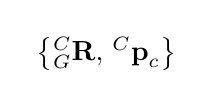
\begin{tikzpicture}[>=stealth,scale=1.1]
  \camprojscene
  \node[below] at (3.10,-0.55) {$\big\{{}^{C}_{G}\vect{R},\,{}^{C}\vect{p}_c\big\}$};
\end{tikzpicture}
\caption{Camera measurement geometry: the feature $\vect{P}_f$ projects through the image plane to the pixel $\vect{z}_c$ in the camera frame $\{C\}$; the global frame $\{G\}$ and the extrinsic $\{{}^{C}_{G}\vect{R},{}^{C}\vect{p}_c\}$ relate the two views of the same point (${}^{C}\vect{p}_f$ vs.\ ${}^{G}\vect{p}_f$).}
\label{fig:lec03-cammodel}
\end{figure}

\paragraph{Simplest pinhole model.} With the feature in the camera frame ${}^{C}\vect{p}_f = [x,\,y,\,z]\trans$, the normalized projection is
\begin{align}
\vect{z}_n = \begin{bmatrix} u_n \\ v_n \end{bmatrix} = \begin{bmatrix} x/z \\ y/z \end{bmatrix},
\qquad
\vect{z}_n = \vect{h}_p({}^{C}\vect{p}_f) + \vect{n}_c, \quad {}^{C}\vect{p}_f = {}^{C}_{G}\vect{R}\trans\big({}^{G}\vect{p}_f - {}^{G}\vect{p}_c\big).
\end{align}
Linearizing the measurement, $\tilde{\vect{z}}_n = \vect{H}_c\,\tilde{\vect{x}} + \vect{n}_c$, with the residual
\begin{align}
\tilde{\vect{z}}_n = \vect{z}_n - \vect{h}_p({}^{C}\hat{\vect{p}}_f) = \begin{bmatrix} u_n \\ v_n \end{bmatrix} - \begin{bmatrix} \hat{x}/\hat{z} \\ \hat{y}/\hat{z} \end{bmatrix}.
\end{align}
The state and its error state are
\begin{align}
\vect{x} : \big\{{}^{C}_{G}\vect{R},\,{}^{G}\vect{p}_c,\,{}^{G}\vect{p}_f\big\}, \quad
{}^{C}_{G}\vect{R} = {}^{C}_{G}\hat{\vect{R}}\,\Exp(\delta\vect{\theta}), \;\;
{}^{G}\vect{p}_c = {}^{G}\hat{\vect{p}}_c + {}^{G}\tilde{\vect{p}}_c, \;\;
{}^{G}\vect{p}_f = {}^{G}\hat{\vect{p}}_f + {}^{G}\tilde{\vect{p}}_f,
\end{align}
with error state $\tilde{\vect{x}} = [\,\delta\vect{\theta}\trans,\; {}^{G}\tilde{\vect{p}}_c\trans,\; {}^{G}\tilde{\vect{p}}_f\trans\,]\trans$.

% =====================================================================
\subsection{The measurement Jacobian}

By the chain rule, factoring every block through ${}^{C}\tilde{\vect{p}}_f$,
\begin{align}
\tilde{\vect{z}}_n &= \vect{H}_c\,\tilde{\vect{x}} + \vect{n}_c \\
&= \begin{bmatrix} \dfrac{\partial\tilde{\vect{z}}_n}{\partial\delta\vect{\theta}} & \dfrac{\partial\tilde{\vect{z}}_n}{\partial{}^{G}\tilde{\vect{p}}_c} & \dfrac{\partial\tilde{\vect{z}}_n}{\partial{}^{G}\tilde{\vect{p}}_f} \end{bmatrix}\tilde{\vect{x}} + \vect{n}_c \\
&= \frac{\partial\tilde{\vect{z}}_n}{\partial{}^{C}\tilde{\vect{p}}_f}\begin{bmatrix} \dfrac{\partial{}^{C}\tilde{\vect{p}}_f}{\partial\delta\vect{\theta}} & \dfrac{\partial{}^{C}\tilde{\vect{p}}_f}{\partial{}^{G}\tilde{\vect{p}}_c} & \dfrac{\partial{}^{C}\tilde{\vect{p}}_f}{\partial{}^{G}\tilde{\vect{p}}_f} \end{bmatrix}\tilde{\vect{x}} + \vect{n}_c.
\end{align}
The projection Jacobian, writing ${}^{C}\vect{p}_f = [c_x,\,c_y,\,c_z]\trans$, is
\begin{align}
\vect{z}_n = \begin{bmatrix} c_x/c_z \\ c_y/c_z \end{bmatrix}, \qquad
\frac{\partial\vect{z}_n}{\partial{}^{C}\vect{p}_f} = \begin{bmatrix} \dfrac{1}{c_z} & 0 & -\dfrac{c_x}{c_z^{2}} \\[2ex] 0 & \dfrac{1}{c_z} & -\dfrac{c_y}{c_z^{2}} \end{bmatrix}
= \frac{1}{c_z^{2}}\begin{bmatrix} c_z & 0 & -c_x \\ 0 & c_z & -c_y \end{bmatrix}.
\end{align}

\paragraph{Perturbing ${}^{C}\vect{p}_f$.} From ${}^{C}\vect{p}_f = {}^{C}_{G}\vect{R}\trans({}^{G}\vect{p}_f - {}^{G}\vect{p}_c)$ with ${}^{C}_{G}\vect{R} = {}^{C}_{G}\hat{\vect{R}}\,\Exp(\delta\vect{\theta})$ and $\Exp(\delta\vect{\theta})\trans \approx \vect{I} - \skewsym{\delta\vect{\theta}}$,
\begin{align}
{}^{C}\hat{\vect{p}}_f + {}^{C}\tilde{\vect{p}}_f
&= \big({}^{C}_{G}\hat{\vect{R}}\,\Exp(\delta\vect{\theta})\big)\trans\big({}^{G}\hat{\vect{p}}_f + {}^{G}\tilde{\vect{p}}_f - {}^{G}\hat{\vect{p}}_c - {}^{G}\tilde{\vect{p}}_c\big) \\
&= \big(\vect{I} - \skewsym{\delta\vect{\theta}}\big)\,{}^{C}_{G}\hat{\vect{R}}\trans\big({}^{G}\hat{\vect{p}}_f + {}^{G}\tilde{\vect{p}}_f - {}^{G}\hat{\vect{p}}_c - {}^{G}\tilde{\vect{p}}_c\big) \\
&\approx {}^{C}_{G}\hat{\vect{R}}\trans\big({}^{G}\hat{\vect{p}}_f - {}^{G}\hat{\vect{p}}_c\big) - \skewsym{\delta\vect{\theta}}\,{}^{C}_{G}\hat{\vect{R}}\trans\big({}^{G}\hat{\vect{p}}_f - {}^{G}\hat{\vect{p}}_c\big) \notag\\
&\quad + {}^{C}_{G}\hat{\vect{R}}\trans\big({}^{G}\tilde{\vect{p}}_f - {}^{G}\tilde{\vect{p}}_c\big).
\end{align}
Using $-\skewsym{\delta\vect{\theta}}\,\vect{a} = \skewsym{\vect{a}}\,\delta\vect{\theta}$ with $\vect{a} = {}^{C}\hat{\vect{p}}_f = {}^{C}_{G}\hat{\vect{R}}\trans({}^{G}\hat{\vect{p}}_f - {}^{G}\hat{\vect{p}}_c)$ and matching hat/tilde terms,
\begin{align}
{}^{C}\hat{\vect{p}}_f + {}^{C}\tilde{\vect{p}}_f
&= \underbrace{{}^{C}_{G}\hat{\vect{R}}\trans\big({}^{G}\hat{\vect{p}}_f - {}^{G}\hat{\vect{p}}_c\big)}_{{}^{C}\hat{\vect{p}}_f}
+ \skewsym{{}^{C}_{G}\hat{\vect{R}}\trans({}^{G}\hat{\vect{p}}_f - {}^{G}\hat{\vect{p}}_c)}\,\delta\vect{\theta} \notag\\
&\quad - {}^{C}_{G}\hat{\vect{R}}\trans\,{}^{G}\tilde{\vect{p}}_c
+ {}^{C}_{G}\hat{\vect{R}}\trans\,{}^{G}\tilde{\vect{p}}_f,
\end{align}
so that, with ${}^{C}\hat{\vect{p}}_f = {}^{C}_{G}\hat{\vect{R}}\trans({}^{G}\hat{\vect{p}}_f - {}^{G}\hat{\vect{p}}_c)$, the three blocks are
\begin{align}
\frac{\partial{}^{C}\tilde{\vect{p}}_f}{\partial\delta\vect{\theta}} = \skewsym{{}^{C}\hat{\vect{p}}_f}, \qquad
\frac{\partial{}^{C}\tilde{\vect{p}}_f}{\partial{}^{G}\tilde{\vect{p}}_c} = -{}^{C}_{G}\hat{\vect{R}}\trans, \qquad
\frac{\partial{}^{C}\tilde{\vect{p}}_f}{\partial{}^{G}\tilde{\vect{p}}_f} = {}^{C}_{G}\hat{\vect{R}}\trans.
\end{align}
Therefore $\tilde{\vect{z}}_n = \vect{H}_c\,\tilde{\vect{x}} + \vect{n}_c$ with
\begin{align}
\vect{H}_c = \frac{1}{c_z^{2}}\begin{bmatrix} c_z & 0 & -c_x \\ 0 & c_z & -c_y \end{bmatrix}
\begin{bmatrix} \skewsym{{}^{C}\hat{\vect{p}}_f} & -{}^{C}_{G}\hat{\vect{R}}\trans & {}^{C}_{G}\hat{\vect{R}}\trans \end{bmatrix}.
\end{align}

% =====================================================================
\subsection{A few important discussions}

\paragraph{(1) SLAM.} The pose $\{{}^{C}_{G}\vect{R},{}^{G}\vect{p}_c\}$ is the localization of the camera, and ${}^{G}\vect{p}_f$ is a 3D feature of the environment. Solving them together means we solve localization and mapping together $\Rightarrow$ \emph{Simultaneous Localization And Mapping} (SLAM).

\paragraph{(2) PnP / P3P --- known feature, solve pose.} If ${}^{G}\vect{p}_f$ is known, given $(u,v)$, how do we solve $\{{}^{C}_{G}\vect{R},{}^{C}\vect{p}_c\}$? Here $\vect{x} : \{{}^{C}_{G}\vect{R},{}^{C}\vect{p}_c\}$ is 6-dof, while each measurement $\vect{z}_n = \vect{h}({}^{C}_{G}\vect{R},{}^{C}\vect{p}_c) + \vect{n}_c$ contributes 2 dof, so we need at least 3 points ${}^{C}\vect{p}_{f_i} \leftrightarrow (u_i,v_i)$ to solve $\{{}^{C}\vect{R},{}^{C}\vect{p}_c\}$.
\begin{itemize}[noitemsep,topsep=2pt]
\item 3 pairs ${}^{C}\vect{p}_{f_i}\leftrightarrow(u_i,v_i)$, \textbf{P3P} (perspective-3-point), i.e.\ $2{+}1$ points: use 3D$\leftrightarrow$3D correspondences to determine the same 3D pose.
\item $n$ pairs of 3D$\leftrightarrow$3D correspondences, \textbf{PnP} (perspective-$n$-point).
\item \textbf{RANSAC} (random sample consensus) for outlier rejection.
\end{itemize}
This is the \emph{structure $\to$ motion} direction (known structure, solve motion).

\paragraph{(3) Triangulation --- known poses, solve feature.} If $\{{}^{C}_{G}\vect{R},{}^{C}\vect{p}_c\}$ is known, given $(u_1,v_1)$, $(u_2,v_2)$, solve $\vect{P}_f$ (Fig.~\ref{fig:lec03-triangulation}). Each pixel gives a unit bearing and an unknown range $r_i$:
\begin{align}
(u_1,v_1)\to {}^{C_1}\vect{b}_1 = \frac{[u_1,v_1,1]\trans}{\norm{[u_1,v_1,1]\trans}}, &\quad
(u_2,v_2)\to {}^{C_2}\vect{b}_2 = \frac{[u_2,v_2,1]\trans}{\norm{[u_2,v_2,1]\trans}}, \\
{}^{C_1}\vect{p}_f = {}^{C_1}\vect{b}_1\, r_1, &\quad {}^{C_2}\vect{p}_f = {}^{C_2}\vect{b}_2\, r_2,
\end{align}
with $r_1,r_2$ unknown. From ${}^{C_1}\vect{p}_f = {}^{C_1}_{C_2}\vect{R}\,{}^{C_2}\vect{p}_f + {}^{C_1}\vect{p}_{C_2}$ we obtain ${}^{C_1}\vect{b}_1\, r_1 = {}^{C_1}_{C_2}\vect{R}\,{}^{C_2}\vect{b}_2\, r_2 + {}^{C_1}\vect{p}_{C_2}$.

\begin{figure}[H]
\centering
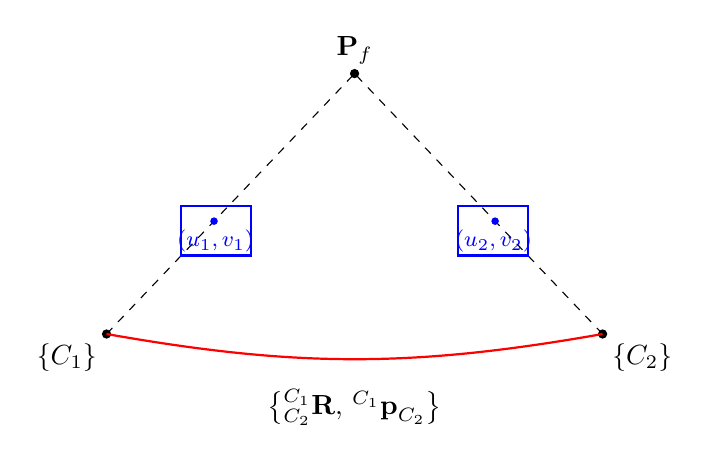
\begin{tikzpicture}[>=stealth,scale=1.05]
  % feature
  \fill (3.0,3.15) circle (1.6pt) node[above] {$\vect{P}_f$};
  % bearing rays
  \draw[dashed] (0,0) -- (3.0,3.15);
  \draw[dashed] (6.0,0) -- (3.0,3.15);
  % image planes (blue) with the pixel where each bearing ray crosses
  \draw[blue,thick] (0.90,0.95) rectangle (1.75,1.55);
  \fill[blue] (1.30,1.365) circle (1.3pt);
  \node[blue] at (1.32,1.12) {\footnotesize $(u_1,v_1)$};
  \draw[blue,thick] (4.25,0.95) rectangle (5.10,1.55);
  \fill[blue] (4.70,1.365) circle (1.3pt);
  \node[blue] at (4.68,1.12) {\footnotesize $(u_2,v_2)$};
  % camera frames
  \fill (0,0) circle (1.6pt); \node[below left] at (0,0) {$\{C_1\}$};
  \fill (6,0) circle (1.6pt); \node[below right] at (6,0) {$\{C_2\}$};
  % baseline
  \draw[red,thick] (0,0) to[bend right=10] (6.0,0);
  \node[below] at (3.0,-0.55) {$\big\{{}^{C_1}_{C_2}\vect{R},\,{}^{C_1}\vect{p}_{C_2}\big\}$};
\end{tikzpicture}
\caption{Two-view triangulation: bearings ${}^{C_1}\vect{b}_1,{}^{C_2}\vect{b}_2$ from pixels $(u_1,v_1),(u_2,v_2)$ and the known relative pose $\{{}^{C_1}_{C_2}\vect{R},{}^{C_1}\vect{p}_{C_2}\}$ fix the feature $\vect{P}_f$ up to the two ranges $r_1,r_2$.}
\label{fig:lec03-triangulation}
\end{figure}

\textbf{Way 1 (stacked linear system).} Collect the two ranges:
\begin{align}
{}^{C_1}\vect{b}_1\, r_1 - {}^{C_1}_{C_2}\vect{R}\,{}^{C_2}\vect{b}_2\, r_2 = {}^{C_1}\vect{p}_{C_2}
\;\Rightarrow\;
\underbrace{\begin{bmatrix} {}^{C_1}\vect{b}_1 & -{}^{C_1}_{C_2}\vect{R}\,{}^{C_2}\vect{b}_2 \end{bmatrix}}_{3\times2}\begin{bmatrix} r_1 \\ r_2 \end{bmatrix} = {}^{C_1}\vect{p}_{C_2},
\end{align}
a $3\times2$ system; solving $r_1,r_2$ gives ${}^{C_1}\vect{p}_f,{}^{C_2}\vect{p}_f$.
\begin{quote}
\textbf{Degenerate case.} If the motion is pure rotation (no translation), then ${}^{C_1}\vect{b}_1 = {}^{C_1}_{C_2}\vect{R}\,{}^{C_2}\vect{b}_2$ and ${}^{C_1}\vect{p}_{C_2} = \vect{0}_{3\times1}$, so $r_1 = r_2$ and there is no way to solve $r$. For a monocular camera, pure rotation is dangerous.
\end{quote}
\textbf{Way 2 (left null space).} With ${}^{C_1}\vect{b}_1\, r_1 = {}^{C_1}_{C_2}\vect{R}\,{}^{C_2}\vect{b}_2\, r_2 + {}^{C_1}\vect{p}_{C_2}$, collect into $\vect{B}^{\perp} = [\,\vect{b}^{\perp_1}\;\;\vect{b}^{\perp_2}\,]$ two directions orthogonal to ${}^{C_1}\vect{b}_1$ (${}^{C_1}\vect{b}_1\trans\vect{b}^{\perp_1} = 0$, ${}^{C_1}\vect{b}_1\trans\vect{b}^{\perp_2} = 0$); projecting removes $r_1$:
\begin{align}
\vect{B}^{\perp\top}\,{}^{C_1}\vect{b}_1\, r_1 = \vect{B}^{\perp\top}\big({}^{C_1}_{C_2}\vect{R}\,{}^{C_2}\vect{b}_2\, r_2 + {}^{C_1}\vect{p}_{C_2}\big) = \vect{0}_{2\times1}
\;\Rightarrow\;
\underbrace{\vect{B}^{\perp\top}\,{}^{C_1}_{C_2}\vect{R}\,{}^{C_2}\vect{b}_2}_{2\times1}\, r_2 = -\underbrace{\vect{B}^{\perp\top}\,{}^{C_1}\vect{p}_{C_2}}_{2\times1}.
\end{align}

\paragraph{(4) Monocular triangulation is up to scale.} If $\{{}^{C}_{G}\vect{R}\}$ is known but for ${}^{C_1}\vect{p}_{C_2}$ we only know the direction $\overrightarrow{{}^{C_1}\vect{p}_{C_2}}$ (with $\norm{{}^{C_1}\vect{p}_{C_2}}$ unknown), can we triangulate ${}^{C}\vect{p}_f$? Let $\norm{{}^{C_1}\vect{p}_{C_2}} = \rho$, then ${}^{C_1}\vect{p}_f = {}^{C_1}_{C_2}\vect{R}\,{}^{C_2}\vect{p}_f + {}^{C_1}\vect{p}_{C_2}$ gives
\begin{align}
{}^{C_1}\vect{b}_1\, r_1 = {}^{C_1}_{C_2}\vect{R}\,{}^{C_2}\vect{b}_2\, r_2 + \rho\,\overrightarrow{{}^{C_1}\vect{p}_{C_2}}.
\end{align}
With $\vect{A} = [\vect{v}^{\perp_1}\;\;\vect{v}^{\perp_2}]\trans$ built from $\overrightarrow{{}^{C_1}\vect{p}_{C_2}}\trans\vect{v}^{\perp_1} = 0,\;\overrightarrow{{}^{C_1}\vect{p}_{C_2}}\trans\vect{v}^{\perp_2} = 0$, projecting kills the translation term:
\begin{align}
\vect{A}\,{}^{C_1}\vect{b}_1\, r_1 &= \vect{A}\,{}^{C_1}_{C_2}\vect{R}\,{}^{C_2}\vect{b}_2\, r_2 + \rho\,\underbrace{\vect{A}\,\overrightarrow{{}^{C_1}\vect{p}_{C_2}}}_{\vect{0}} \\
\Rightarrow\;\;
\begin{bmatrix} \vect{A}\,{}^{C_1}\vect{b} & -\vect{A}\,{}^{C_1}_{C_2}\vect{R}\,{}^{C_2}\vect{b} \end{bmatrix}\begin{bmatrix} r_1 \\ r_2 \end{bmatrix} &= \vect{0}.
\end{align}
Hence $r_1,r_2$ are up to scale: a monocular camera does not have scale. The above uses \emph{motion to infer structure}.

\paragraph{(5) Essential matrix --- solve the motion.} Given $\{u_1,v_1\},\{u_2,v_2\}$, can we solve $\{{}^{C}_{G}\vect{R},{}^{C}\vect{p}_c\}$? The three vectors ${}^{C_1}\vect{p}_f$, ${}^{C_2}\vect{p}_f$, ${}^{C_1}\vect{p}_{C_2}$ are coplanar (Fig.~\ref{fig:lec03-epipolar}), so ${}^{C_1}\vect{p}_{C_2}\times{}^{C_1}\vect{p}_f \perp {}^{C_1}_{C_2}\vect{R}\,{}^{C_2}\vect{p}_f$:
\begin{align}
\big(\skewsym{{}^{C_1}\vect{p}_{C_2}}\,{}^{C_1}\vect{p}_f\big)\trans {}^{C_1}_{C_2}\vect{R}\,{}^{C_2}\vect{p}_f = 0
\;\Rightarrow\;
{}^{C_1}\vect{p}_f\trans\,\skewsym{{}^{C_1}\vect{p}_{C_2}}\,{}^{C_1}_{C_2}\vect{R}\,{}^{C_2}\vect{p}_f = 0.
\end{align}
With ${}^{C_1}\vect{p}_f = {}^{C_1}\vect{b}\,r_1$, ${}^{C_2}\vect{p}_f = {}^{C_2}\vect{b}\,r_2$,
\begin{empheq}[box=\fbox]{align}
{}^{C_1}\vect{b}\trans\,\skewsym{{}^{C_1}\vect{p}_{C_2}}\,{}^{C_1}_{C_2}\vect{R}\,{}^{C_2}\vect{b} = 0, \qquad
\vect{E} = \skewsym{{}^{C_1}\vect{p}_{C_2}}\,{}^{C_1}_{C_2}\vect{R} \quad\text{(essential matrix)}.
\end{empheq}

\begin{figure}[H]
\centering
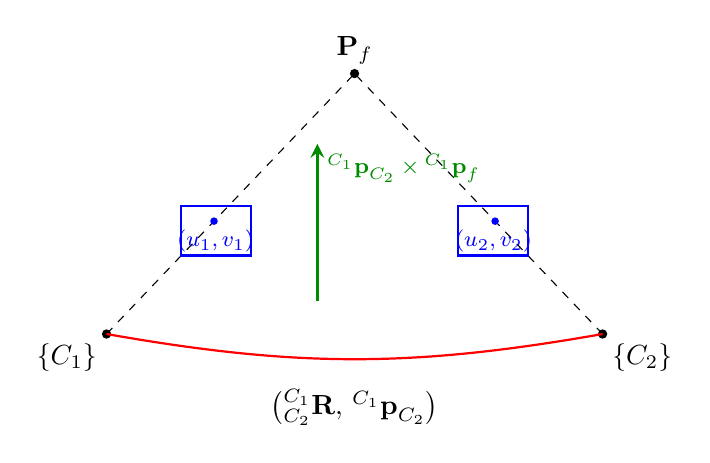
\begin{tikzpicture}[>=stealth,scale=1.05]
  \fill (3.0,3.15) circle (1.6pt) node[above] {$\vect{P}_f$};
  \draw[dashed] (0,0) -- (3.0,3.15);
  \draw[dashed] (6.0,0) -- (3.0,3.15);
  % image planes with pixels
  \draw[blue,thick] (0.90,0.95) rectangle (1.75,1.55);
  \fill[blue] (1.30,1.365) circle (1.3pt);
  \node[blue] at (1.32,1.12) {\footnotesize $(u_1,v_1)$};
  \draw[blue,thick] (4.25,0.95) rectangle (5.10,1.55);
  \fill[blue] (4.70,1.365) circle (1.3pt);
  \node[blue] at (4.68,1.12) {\footnotesize $(u_2,v_2)$};
  % camera frames
  \fill (0,0) circle (1.6pt); \node[below left] at (0,0) {$\{C_1\}$};
  \fill (6,0) circle (1.6pt); \node[below right] at (6,0) {$\{C_2\}$};
  \draw[red,thick] (0,0) to[bend right=10] (6.0,0);
  % normal of the epipolar plane (the cross product)
  \draw[->,very thick,green!55!black] (2.55,0.40) -- (2.55,2.30);
  \node[green!55!black,right] at (2.55,2.00) {\footnotesize ${}^{C_1}\vect{p}_{C_2}\times{}^{C_1}\vect{p}_f$};
  \node[below] at (3.0,-0.55) {$\big({}^{C_1}_{C_2}\vect{R},\,{}^{C_1}\vect{p}_{C_2}\big)$};
\end{tikzpicture}
\caption{Epipolar geometry: ${}^{C_1}\vect{p}_f$, ${}^{C_2}\vect{p}_f$, and the baseline ${}^{C_1}\vect{p}_{C_2}$ are coplanar, giving the essential-matrix constraint ${}^{C_1}\vect{b}\trans\vect{E}\,{}^{C_2}\vect{b} = 0$.}
\label{fig:lec03-epipolar}
\end{figure}

Why is $\vect{E}$ 5-dof? Each pair $(u_1,v_1),(u_2,v_2)$ provides 1 constraint, so we need at least \textbf{5 pairs of points} to solve $\vect{E} \Rightarrow {}^{C_1}_{C_2}\vect{R}$ (3 dof) and $\overrightarrow{{}^{C_1}\vect{p}_{C_2}}$ (2 dof, direction only). When selecting pairs of points, RANSAC (random sample consensus) comes in. Finally:
\begin{align}
\text{normalized coordinates:} \;\; & {}^{C_1}\vect{b}\trans\skewsym{{}^{C_1}\vect{p}_{C_2}}\,{}^{C_1}_{C_2}\vect{R}\,{}^{C_2}\vect{b} = 0 \;\;(\text{essential matrix}), \\
\text{pixel coordinates:} \;\; & \text{fundamental matrix}.
\end{align}
This is the \emph{motion from structure} direction.

% =====================================================================
\subsection{The full intrinsic calibration model}

The calibration geometry is the same as Fig.~\ref{fig:lec03-cammodel} (repeated here as Fig.~\ref{fig:lec03-calib}). The camera model is a composition of four functions.

\begin{figure}[H]
\centering
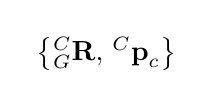
\begin{tikzpicture}[>=stealth,scale=1.1]
  \camprojscene
  \node[below] at (3.10,-0.55) {$\big\{{}^{C}_{G}\vect{R},\,{}^{C}\vect{p}_c\big\}$};
\end{tikzpicture}
\caption{The intrinsic calibration sits inside the same projection geometry: the 3D feature is transformed into $\{C\}$, projected, distorted, and mapped to pixels.}
\label{fig:lec03-calib}
\end{figure}

\paragraph{Projection and transform.}
\begin{align}
\vect{z}_n = \begin{bmatrix} c_x/c_z \\ c_y/c_z \end{bmatrix} \triangleq \vect{h}_p({}^{C}\vect{p}_f), &\qquad
{}^{C}\vect{p}_f = {}^{C}_{G}\vect{R}\trans({}^{G}\vect{p}_f - {}^{G}\vect{p}_c) \triangleq \vect{h}_t({}^{C}_{G}\vect{R},{}^{G}\vect{p}_c,{}^{G}\vect{p}_f), \\
\vect{z}_n &= \vect{h}_p\big(\vect{h}_t({}^{C}_{G}\vect{R},{}^{G}\vect{p}_c,{}^{G}\vect{p}_f)\big) + \vect{n}.
\end{align}
\paragraph{Distortion.} Radial-tangential (for example); fisheye uses the equidistant model. With $r^{2} = u_n^{2} + v_n^{2}$ and distortion parameters $\vect{x}_d = [k_1,k_2,p_1,p_2]\trans$,
\begin{align}
\begin{bmatrix} u_d \\ v_d \end{bmatrix}
= \begin{bmatrix} u_n \\ v_n \end{bmatrix}\big(1 + k_1 r^{2} + k_2 r^{4}\big)
+ \begin{bmatrix} 2 p_1 u_n v_n + p_2\,(r^{2} + 2 u_n^{2}) \\ p_1\,(r^{2} + 2 v_n^{2}) + 2 p_2 u_n v_n \end{bmatrix}, \qquad
\vect{z}_d = \begin{bmatrix} u_d \\ v_d \end{bmatrix} = \vect{h}_d(\vect{z}_n).
\end{align}
\paragraph{Intrinsics / homography.} With $\vect{x}_{in} = [f_u,f_v,c_u,c_v]$,
\begin{align}
\begin{bmatrix} u \\ v \\ 1 \end{bmatrix}
= \underbrace{\begin{bmatrix} f_u & 0 & c_u \\ 0 & f_v & c_v \\ 0 & 0 & 1 \end{bmatrix}}_{\vect{K}}\begin{bmatrix} u_d \\ v_d \\ 1 \end{bmatrix}, \qquad
\vect{z} = \begin{bmatrix} u \\ v \end{bmatrix} = \begin{bmatrix} f_u & 0 \\ 0 & f_v \end{bmatrix}\begin{bmatrix} u_d \\ v_d \end{bmatrix} + \begin{bmatrix} c_u \\ c_v \end{bmatrix} \triangleq \vect{h}_k(\vect{z}_d,\vect{x}_{in}).
\end{align}
\paragraph{Full composition.}
\begin{align}
\vect{z}_c = \vect{h}_c(\vect{x}) + \vect{n}_c
&= \vect{h}_k(\vect{z}_d,\vect{x}_{in}) + \vect{n}_c \\
&= \vect{h}_k\big(\vect{h}_d(\vect{z}_n,\vect{x}_d),\vect{x}_{in}\big) + \vect{n}_c \\
&= \vect{h}_k\big(\vect{h}_d(\vect{h}_p({}^{C}\vect{p}_f),\vect{x}_d),\vect{x}_{in}\big) + \vect{n}_c \\
&= \vect{h}_k\Big(\vect{h}_d\big(\vect{h}_p(\vect{h}_t({}^{C}_{G}\vect{R},{}^{G}\vect{p}_c,{}^{G}\vect{p}_f)),\vect{x}_d\big),\vect{x}_{in}\Big) + \vect{n}_c,
\end{align}
where $\vect{h}_k(\cdot)$ is the camera-intrinsics homography, $\vect{h}_d(\cdot)$ the distortion function, $\vect{h}_p(\cdot)$ the projection function, $\vect{h}_t(\cdot)$ the transform function, $\vect{x}_d$ the distortion parameters, and $\vect{x}_{in}=\{f_u,f_v,c_u,c_v\}$ the intrinsics. The Jacobians for calibration follow by the chain rule.

% =====================================================================
\subsection{The extrinsic (camera--IMU) calibration}

The camera and IMU sensor frames are rigidly connected (Fig.~\ref{fig:lec03-extrinsic}).

\begin{figure}[H]
\centering
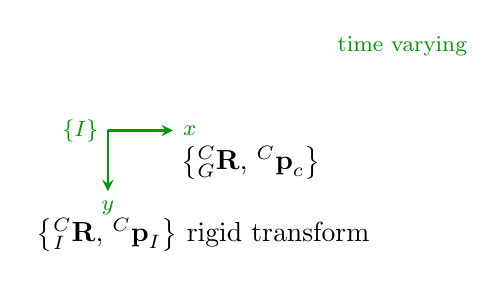
\begin{tikzpicture}[>=stealth,scale=1.1]
  \camprojscene
  % IMU frame {I}, rigidly attached near {C} (offset clearly below the camera axes)
  \draw[->,thick,green!60!black] (1.45,-0.55) -- (2.20,-0.55) node[right] {\footnotesize $x$};
  \draw[->,thick,green!60!black] (1.45,-0.55) -- (1.45,-1.25) node[below] {\footnotesize $y$};
  \node[green!60!black,left] at (1.45,-0.55) {\footnotesize $\{I\}$};
  \node[green!60!black] at (4.85,0.42) {\footnotesize time varying};
  \node[below] at (3.10,-0.62) {$\big\{{}^{C}_{G}\vect{R},\,{}^{C}\vect{p}_c\big\}$};
  \node[below] at (2.55,-1.45) {$\big\{{}^{C}_{I}\vect{R},\,{}^{C}\vect{p}_I\big\}$ rigid transform};
\end{tikzpicture}
\caption{Extrinsic calibration: the IMU frame $\{I\}$ is rigidly fixed to the camera $\{C\}$ via $\{{}^{C}_{I}\vect{R},{}^{C}\vect{p}_I\}$, while the camera-to-global transform is time varying.}
\label{fig:lec03-extrinsic}
\end{figure}

\begin{align}
\begin{bmatrix} {}^{C}\vect{p}_f \\ 1 \end{bmatrix}
&= \underbrace{\begin{bmatrix} {}^{C}_{I}\vect{R} & {}^{C}\vect{p}_I \\ \vect{0}_{1\times3} & 1 \end{bmatrix}}_{{}^{C}_{I}\vect{T}}
\underbrace{\begin{bmatrix} {}^{G}_{I}\vect{R} & {}^{G}\vect{p}_I \\ \vect{0}_{1\times3} & 1 \end{bmatrix}^{-1}}_{{}^{G}_{I}\vect{T}^{-1}}
\begin{bmatrix} {}^{G}\vect{p}_f \\ 1 \end{bmatrix}, \\
{}^{C}\vect{p}_f &= {}^{C}_{I}\vect{R}\,{}^{I}\vect{p}_f + {}^{C}\vect{p}_I = {}^{C}_{I}\vect{R}\big({}^{I}_{G}\vect{R}({}^{G}\vect{p}_f - {}^{G}\vect{p}_I)\big) + {}^{C}\vect{p}_I.
\end{align}

\paragraph{Time offset.} How do we estimate the time offset between camera and IMU? With $t_I = t_c + t_d$,
\begin{align}
\begin{bmatrix} {}^{C_{t_c}}\vect{p}_f \\ 1 \end{bmatrix} &= {}^{C}_{I}\vect{T}\cdot\big({}^{G}_{I(t+t_d)}\vect{T}\big)^{-1}\begin{bmatrix} {}^{G}\vect{p}_f \\ 1 \end{bmatrix}, \\
{}^{G}_{I(t+t_d)}\dot{\vect{T}} &= \begin{bmatrix} {}^{G}_{I}\vect{R} & {}^{G}\vect{p}_I \\ \vect{0}_{1\times3} & 1 \end{bmatrix}\begin{bmatrix} \skewsym{{}^{I}\vect{\omega}} & {}^{I}\vect{v} \\ \vect{0}_{1\times3} & 0 \end{bmatrix}.
\end{align}
which is the Jacobian for $t_d$. This is then the full calibration for the vision system.

% =====================================================================
\subsection{Point / line / plane representation}

\subsubsection{Point representation}
In $\Reals^{3}$ (closest point),
\begin{align}
\vect{P}_f = \begin{bmatrix} x \\ y \\ z \end{bmatrix} = z\begin{bmatrix} x/z \\ y/z \\ 1 \end{bmatrix} = z\begin{bmatrix} u_n \\ v_n \\ 1 \end{bmatrix}.
\end{align}
\paragraph{Inverse depth.} Store the inverse of the depth, $\lambda \triangleq 1/z$:
\begin{align}
\vect{x}_f = \begin{bmatrix} x \\ y \\ 1/z \end{bmatrix} = \begin{bmatrix} x \\ y \\ \lambda \end{bmatrix}.
\end{align}
\emph{What is the motivation to use inverse depth?} Transform the feature into a second view and divide by $z$:
\begin{align}
{}^{C_2}\vect{p}_f &= {}^{C_2}_{C_1}\vect{R}\big({}^{C_1}\vect{p}_f - {}^{C_1}\vect{p}_{C_2}\big)
= {}^{C_2}_{C_1}\vect{R}\Big(\begin{bmatrix} x \\ y \\ z \end{bmatrix} - {}^{C_1}\vect{p}_{C_2}\Big)
= {}^{C_2}_{C_1}\vect{R}\Big(z\begin{bmatrix} x/z \\ y/z \\ 1 \end{bmatrix} - {}^{C_1}\vect{p}_{C_2}\Big), \\
\frac{{}^{C_2}\vect{p}_f}{z} &= {}^{C_2}_{C_1}\vect{R}\Big(\begin{bmatrix} x/z \\ y/z \\ 1 \end{bmatrix} - \frac{1}{z}{}^{C_1}\vect{p}_{C_2}\Big)
\;\Rightarrow\;
\begin{bmatrix} {}^{C_2}x/z \\ {}^{C_2}y/z \\ {}^{C_2}z/z \end{bmatrix} = {}^{C_2}_{C_1}\vect{R}\Big(\begin{bmatrix} x\lambda \\ y\lambda \\ 1 \end{bmatrix} - \lambda\,{}^{C_1}\vect{p}_{C_2}\Big).
\end{align}
If $z\to\infty$, the feature is far away, $z\approx{}^{C_2}z \gg {}^{C_2}x,{}^{C_2}y$, then the left side tends to the bearing measurement in $\{C_2\}$:
\begin{align}
\begin{bmatrix} {}^{C_2}x/z \\ {}^{C_2}y/z \\ {}^{C_2}z/z \end{bmatrix} \approx \underbrace{\begin{bmatrix} u_{n_2} \\ v_{n_2} \\ 1 \end{bmatrix}}_{\text{measurements in } C_2} \propto {}^{C_2}_{C_1}\vect{R}\Big(\begin{bmatrix} x\lambda \\ y\lambda \\ 1 \end{bmatrix} - \lambda\,{}^{C_1}\vect{p}_{C_2}\Big).
\end{align}
The Jacobian with respect to the inverse-depth state $\tilde{\vect{x}} = [\tilde x,\tilde y,\tilde\lambda]$ is
\begin{align}
\frac{\partial[u_{n_2};v_{n_2}]}{\partial\tilde{\vect{x}}}
= \begin{bmatrix} 1 & 0 & 0 \\ 0 & 1 & 0 \end{bmatrix}\begin{bmatrix} \vect{H}_\theta & \vect{H}_p & \vect{H}_{p_f} \end{bmatrix},
\end{align}
with the three blocks
\begin{align}
\vect{H}_\theta &= \skewsym{{}^{C_2}_{C_1}\vect{R}\big([x\lambda;\,y\lambda;\,1] - \lambda\,{}^{C_1}\vect{p}_{C_2}\big)}, \qquad
\vect{H}_p = \underbrace{-\lambda\,{}^{C_2}_{C_1}\vect{R}}_{\lambda\to0}, \\
\vect{H}_{p_f} &= {}^{C_2}_{C_1}\vect{R}\big[\,\underbrace{\lambda\vect{e}_1}_{0} \;\; \underbrace{\lambda\vect{e}_2}_{0} \;\; [x;\,y;\,0]-{}^{C_1}\vect{p}_{C_2}\,\big].
\end{align}
If the feature is far away, then the rotation is improved, but the Jacobian for translation will not be improved (the $-\lambda\,{}^{C_2}_{C_1}\vect{R}$ and $\lambda\vect{e}_1,\lambda\vect{e}_2$ columns vanish as $\lambda\to0$).

\subsubsection{Plane representation}
A plane is parameterized by its normal direction and distance to the origin (Fig.~\ref{fig:lec03-plane}):
\begin{align}
\vect{\pi} = \begin{bmatrix} \vect{n}_\pi \\ d_\pi \end{bmatrix}_{4\times1}, \qquad
\vect{n}_\pi : \text{normal direction}, \quad d_\pi : \text{distance to origin}.
\end{align}
A plane is 3-dof but $\vect{\pi}$ has 4 parameters. The \emph{closest-point representation} packs both into one vector,
\begin{align}
\vect{P}_\pi = d_\pi\,\vect{n}_\pi = \begin{bmatrix} x \\ y \\ z \end{bmatrix},
\end{align}
the closest point from the plane to the origin.

\begin{figure}[H]
\centering
\begin{subfigure}[b]{0.46\textwidth}
\centering
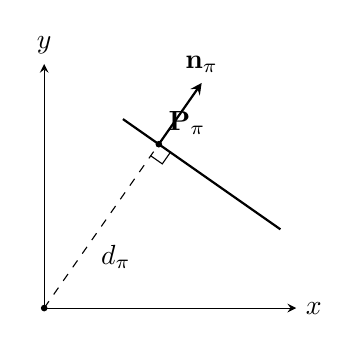
\begin{tikzpicture}[>=stealth,scale=1.0]
  \draw[->] (0,0) -- (3.2,0) node[right] {$x$};
  \draw[->] (0,0) -- (0,3.1) node[above] {$y$};
  \fill (0,0) circle (1.2pt);
  % plane (a line in 2D)
  \draw[thick] (1.0,2.4) -- (3.0,1.0);
  % P_pi = foot of the perpendicular from the origin; d_pi and n_pi are collinear (both normal to the plane)
  \coordinate (P) at (1.456,2.081);
  \draw[dashed] (0,0) -- (P);
  \node[below right] at (0.60,0.92) {$d_\pi$};
  \fill (P) circle (1.2pt); \node[above right] at (P) {$\vect{P}_\pi$};
  \draw[->,thick] (P) -- ($(P)+(0.544,0.778)$) node[above] {$\vect{n}_\pi$};
  % right-angle mark: d_pi is perpendicular to the plane
  \draw ($(P)+(-0.103,-0.147)$) -- ($(P)+(0.044,-0.250)$) -- ($(P)+(0.147,-0.103)$);
\end{tikzpicture}
\caption{plane: $\vect{n}_\pi$, $d_\pi$, foot $\vect{P}_\pi$}
\label{fig:lec03-plane}
\end{subfigure}
\hfill
\begin{subfigure}[b]{0.50\textwidth}
\centering
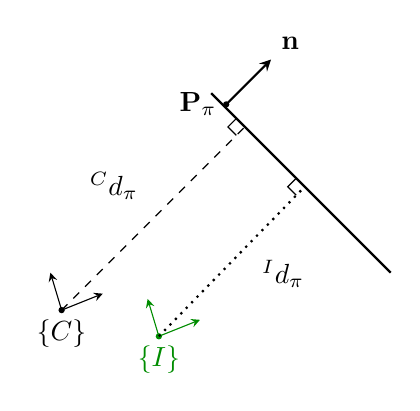
\begin{tikzpicture}[>=stealth,scale=0.95]
  % plane (a line); outward normal points up-right at 45 deg
  \coordinate (Pa) at (5.2,1.5);
  \coordinate (Pb) at (2.8,3.9);
  \draw[thick] (Pa) -- (Pb);
  % a marked point on the plane carrying the normal
  \coordinate (Pn) at (3.0,3.75);
  \fill (Pn) circle (1.2pt); \node[left] at (Pn) {$\vect{P}_\pi$};
  \draw[->,thick] (Pn) -- ($(Pn)+(0.6,0.6)$) node[above right] {$\vect{n}$};
  % camera frame {C} (small triad)
  \coordinate (C) at (0.8,1.0);
  \fill (C) circle (1.2pt);
  \draw[->] (C) -- ($(C)+(0.55,0.22)$); \draw[->] (C) -- ($(C)+(-0.15,0.5)$);
  \node[below] at (C) {$\{C\}$};
  % IMU frame {I} (green triad, rigidly attached)
  \coordinate (I) at (2.1,0.65);
  \fill[green!55!black] (I) circle (1.2pt);
  \draw[->,green!55!black] (I) -- ($(I)+(0.55,0.22)$); \draw[->,green!55!black] (I) -- ($(I)+(-0.15,0.5)$);
  \node[green!55!black,below] at (I) {$\{I\}$};
  % perpendicular distances to the plane (parallel, along the normal, distinct feet)
  \coordinate (Fc) at (3.249,3.449);
  \coordinate (Fi) at (4.049,2.649);
  \draw[dashed] (C) -- (Fc); \node[above left] at (1.95,2.35) {${}^{C}d_\pi$};
  \draw[dotted,thick] (I) -- (Fi); \node[below right] at (3.35,1.80) {${}^{I}d_\pi$};
  % right-angle marks at the feet
  \draw ($(Fc)+(-0.113,-0.113)$) -- ($(Fc)+(-0.226,0)$) -- ($(Fc)+(-0.113,0.113)$);
  \draw ($(Fi)+(-0.113,-0.113)$) -- ($(Fi)+(-0.226,0)$) -- ($(Fi)+(-0.113,0.113)$);
\end{tikzpicture}
\caption{transfer the plane $\{C\}\to\{I\}$}
\label{fig:lec03-planetransfer}
\end{subfigure}
\caption{Plane representation (a) and its transfer between the camera and IMU frames (b).}
\end{figure}

\paragraph{Transfer $\{C\}\to\{I\}$.} For ${}^{C}\vect{p}_\pi \leftrightarrow {}^{I}\vect{p}_\pi$ (Fig.~\ref{fig:lec03-planetransfer}),
\begin{align}
\begin{cases}
{}^{I}\vect{n}_\pi = {}^{I}_{C}\vect{R}\,{}^{C}\vect{n}_\pi & \Rightarrow \text{normal direction} \\[2pt]
{}^{I}d_\pi = {}^{C}d_\pi - {}^{C}\vect{n}_\pi\trans\cdot{}^{C}\vect{p}_I & \Rightarrow \text{origin to plane}
\end{cases}
\end{align}
Hence, using ${}^{I}d_\pi = {}^{C}d_\pi - {}^{C}\vect{p}_I\trans\,{}^{C}\vect{n}_\pi$ and ${}^{C}\vect{p}_I = -{}^{C}_{I}\vect{R}\,{}^{I}\vect{p}_C$ (so $-{}^{C}\vect{p}_I\trans = {}^{I}\vect{p}_C\trans\,{}^{I}_{C}\vect{R}$),
\begin{align}
\begin{bmatrix} {}^{I}\vect{n}_\pi \\ {}^{I}d_\pi \end{bmatrix} = \begin{bmatrix} {}^{I}_{C}\vect{R} & \vect{0}_{3\times1} \\ -{}^{C}\vect{p}_I\trans & 1 \end{bmatrix}\begin{bmatrix} {}^{C}\vect{n}_\pi \\ {}^{C}d_\pi \end{bmatrix}
= \begin{bmatrix} {}^{I}_{C}\vect{R} & \vect{0}_{3\times1} \\ {}^{I}\vect{p}_C\trans\,{}^{I}_{C}\vect{R} & 1 \end{bmatrix}\begin{bmatrix} {}^{C}\vect{n}_\pi \\ {}^{C}d_\pi \end{bmatrix}.
\end{align}
The transformation chain is therefore
\begin{align}
{}^{G}\vect{p}_\pi \to ({}^{C}\vect{n}_\pi,{}^{C}d_\pi) \to ({}^{I}_{C}\vect{R},{}^{I}\vect{p}_C) \to ({}^{I}\vect{n}_\pi,{}^{I}d_\pi) \to {}^{I}\vect{p}_\pi.
\end{align}

\subsubsection{Line representation}
How do we represent a 3D line (Fig.~\ref{fig:lec03-line3d})? For a line $L$: $\vect{v}_e$ is the 3D direction, $d_L$ is the distance from the origin to the line, and $\vect{n}_e$ is the normal direction of the plane (through the line and the origin).

\begin{figure}[H]
\centering
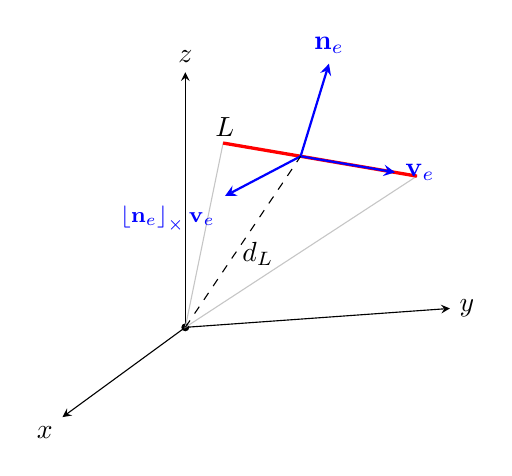
\begin{tikzpicture}[>=stealth,scale=1.2]
  % 3D axes
  \draw[->] (0,0) -- (0,2.7) node[above] {$z$};
  \draw[->] (0,0) -- (2.8,0.2) node[right] {$y$};
  \draw[->] (0,0) -- (-1.3,-0.95) node[below left] {$x$};
  \fill (0,0) circle (1.2pt);
  % plane through the line and the origin (faint triangle)
  \coordinate (A) at (0.40,1.95);
  \coordinate (B) at (2.45,1.60);
  \draw[gray!45] (0,0) -- (A) -- (B) -- cycle;
  % the line L (red)
  \draw[red,very thick] (A) -- (B);
  \node[above left,black] at (0.62,1.92) {$L$};
  % anchor M = closest point of the line to the origin (foot of d_L)
  \coordinate (M) at (1.22,1.81);
  % orthonormal frame {n_e, v_e, <n_e>x v_e} at M
  \draw[->,thick,blue] (M) -- ($(M)+(1.00,-0.17)$) node[right] {$\vect{v}_e$};            % along the line
  \draw[->,thick,blue] (M) -- ($(M)+(0.30,0.98)$) node[above] {$\vect{n}_e$};               % plane normal
  \draw[->,thick,blue] (M) -- ($(M)+(-0.80,-0.42)$) node[below left] {\footnotesize $\skewsym{\vect{n}_e}\vect{v}_e$};
  % perpendicular distance d_L from origin to the line
  \draw[dashed] (0,0) -- (M); \node[right] at (0.50,0.78) {$d_L$};
\end{tikzpicture}
\caption{3D line $L$: direction $\vect{v}_e$, plane normal $\vect{n}_e$, third axis $\skewsym{\vect{n}_e}\vect{v}_e$, and perpendicular distance $d_L$ from the origin.}
\label{fig:lec03-line3d}
\end{figure}

We can represent a line with $\{\vect{n}_e,\vect{v}_e,d_L\}$, where
\begin{align}
\vect{R}_L = \begin{bmatrix} \vect{n}_e & \vect{v}_e & \skewsym{\vect{n}_e}\vect{v}_e \end{bmatrix} \;\text{(a rotation matrix)}, \qquad d_L \;\text{(a distance scalar)}.
\end{align}
So $L : \{\vect{R}_L,d_L\} : \{\bar{\vect{q}}_L,d_L\}$, packed as the 4D vector $\vect{P}_L = \bar{\vect{q}}_L\cdot d_L$, with the error states in Euclidean space. Then
\begin{align}
\vect{P}_L = \hat{\vect{P}}_L + \tilde{\vect{P}}_L
&= \bar{\vect{q}}_L\cdot d_L = \hat{\bar{\vect{q}}}_L \otimes \delta\vect{q}_L\cdot(\hat d_L + \tilde d_L) \\
\Leftrightarrow\; \hat{\vect{P}}_L + \tilde{\vect{P}}_L &= \hat{\bar{\vect{q}}}_L \otimes \begin{bmatrix} 1 \\ \tfrac12\delta\vect{\theta}_L \end{bmatrix}(\hat d_L + \tilde d_L) \\
&= \hat{\bar{\vect{q}}}_L \otimes \begin{bmatrix} \hat d_L + \tilde d_L \\ \tfrac12\hat d_L\,\delta\vect{\theta}_L \end{bmatrix} \\
&= \hat{\bar{\vect{q}}}_L \otimes \Big(\begin{bmatrix} \hat d_L \\ \vect{0}_{3\times1} \end{bmatrix} + \begin{bmatrix} 1 & \vect{0} \\ \vect{0} & \tfrac12\hat d_L\vect{I}_3 \end{bmatrix}\begin{bmatrix} \tilde d_L \\ \delta\vect{\theta}_L \end{bmatrix}\Big),
\end{align}
so that, with $\lfloor\hat{\bar{\vect{q}}}_L\rfloor_L$ the left quaternion-product matrix,
\begin{empheq}[box=\fbox]{align}
\tilde{\vect{P}}_L = \big\lfloor\hat{\bar{\vect{q}}}_L\big\rfloor_L\begin{bmatrix} 1 & \vect{0} \\ \vect{0} & \tfrac12\hat d_L\vect{I}_3 \end{bmatrix}\begin{bmatrix} \tilde d_L \\ \delta\vect{\theta}_L \end{bmatrix}.
\end{empheq}

\paragraph{A few discussions on lines with cameras.}

\textbf{(1) How to project a 3D line to a 2D line in the image?} Given a line $\{\vect{n}_e,\vect{v}_e,d_L\}$ and camera parameters $f_u,f_v,c_u,c_v$ (Fig.~\ref{fig:lec03-lineproj}):
\begin{align}
\begin{bmatrix} u_n \\ v_n \\ 1 \end{bmatrix} \sim \underbrace{\begin{bmatrix} f_u & 0 & c_u \\ 0 & f_v & c_v \\ 0 & 0 & 1 \end{bmatrix}}_{\vect{K}}\underbrace{\begin{bmatrix} x \\ y \\ z \end{bmatrix}}_{\vect{p}_f}, \qquad
\underbrace{\vect{p}}_{\text{pixel on image}} \sim \vect{K}\,\vect{p}_f.
\end{align}
Every $\vect{p}_f$ on the line lies in the plane through the line and the origin, so $\vect{p}_f\trans\vect{n}_e = 0$. With $\vect{p}_f \sim \vect{K}^{-1}\vect{p}$,
\begin{align}
(\vect{K}^{-1}\vect{p})\trans\vect{n}_e = 0 \;\Rightarrow\; \vect{p}\trans\vect{K}^{-\top}\vect{n}_e = 0 \;\Rightarrow\; \vect{n}_e\trans\vect{K}^{-1}\vect{p} = 0 \;\Rightarrow\; (\vect{K}^{-\top}\vect{n}_e)\trans\vect{p} = 0,
\end{align}
so the 2D image line is
\begin{align}
\vect{l} = \vect{K}^{-\top}\vect{n}_e, \qquad \vect{p} \text{ is every pixel on the line}.
\end{align}

\begin{figure}[H]
\centering
\begin{subfigure}[b]{0.46\textwidth}
\centering
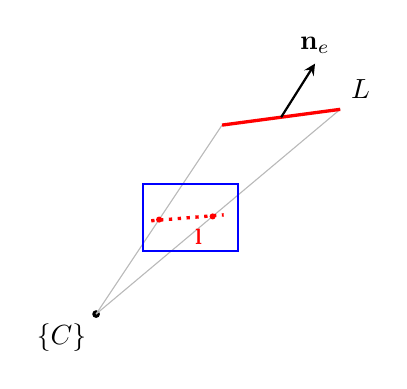
\begin{tikzpicture}[>=stealth,scale=1.0]
  \fill (0,0) circle (1.4pt); \node[below left] at (0,0) {$\{C\}$};
  % the 3D line L and the two sight rays from {C} to its endpoints
  \coordinate (A) at (1.6,2.4);
  \coordinate (B) at (3.1,2.6);
  \draw[gray!55] (0,0) -- (A); \draw[gray!55] (0,0) -- (B);
  \draw[red,very thick] (A) -- (B) node[above right,black] {$L$};
  % normal of the plane through {C} and L
  \draw[->,thick] (2.35,2.5) -- (2.78,3.18) node[above] {$\vect{n}_e$};
  % image plane
  \draw[blue,thick] (0.6,0.8) rectangle (1.8,1.65);
  % projected image line l = where the (C,L) plane meets the image plane
  \fill[red] (0.80,1.20) circle (1.1pt); \fill[red] (1.48,1.24) circle (1.1pt);
  \draw[red,dotted,very thick] (0.70,1.185) -- (1.62,1.26);
  \node[red] at (1.30,0.98) {\footnotesize $\vect{l}$};
\end{tikzpicture}
\caption{project 3D line $\to$ image line $\vect{l}=\vect{K}^{-\top}\vect{n}_e$}
\label{fig:lec03-lineproj}
\end{subfigure}
\hfill
\begin{subfigure}[b]{0.50\textwidth}
\centering
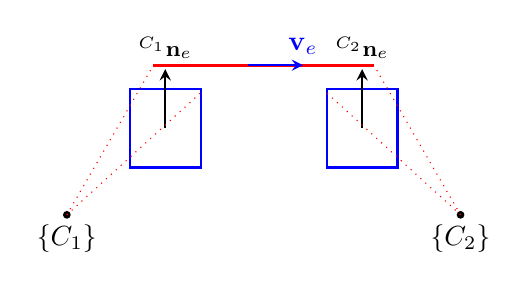
\begin{tikzpicture}[>=stealth,scale=1.0]
  \fill (0,0) circle (1.4pt); \node[below] at (0,0) {$\{C_1\}$};
  \fill (5.0,0) circle (1.4pt); \node[below] at (5.0,0) {$\{C_2\}$};
  % image planes
  \draw[blue,thick] (0.8,0.6) rectangle (1.7,1.6);
  \draw[blue,thick] (3.3,0.6) rectangle (4.2,1.6);
  % 3D line viewed from both (red), shared direction v_e
  \draw[red,very thick] (1.1,1.9) -- (3.9,1.9);
  \draw[->,thick,blue] (2.3,1.9) -- (3.0,1.9) node[above] {$\vect{v}_e$};
  % per-image normals
  \draw[->,thick] (1.25,1.1) -- (1.25,1.85) node[above] {\footnotesize ${}^{C_1}\vect{n}_e$};
  \draw[->,thick] (3.75,1.1) -- (3.75,1.85) node[above] {\footnotesize ${}^{C_2}\vect{n}_e$};
  % rays from the camera centres
  \draw[red,dotted] (0,0) -- (1.1,1.9); \draw[red,dotted] (0,0) -- (1.7,1.55);
  \draw[red,dotted] (5.0,0) -- (3.9,1.9); \draw[red,dotted] (5.0,0) -- (3.3,1.55);
\end{tikzpicture}
\caption{transfer a line $\{C_1\}\to\{C_2\}$}
\label{fig:lec03-linetransfer}
\end{subfigure}
\caption{Lines with cameras: projecting a 3D line to a 2D image line (a) and transferring a line between two camera frames (b).}
\end{figure}

\textbf{(2) How to transfer a line from frame $\{C_1\}$ to $\{C_2\}$?} (Fig.~\ref{fig:lec03-linetransfer}) The line $L$ is given by ${}^{C_1}\vect{n}_e$, ${}^{C_1}\vect{v}_e$, ${}^{C_1}d_L$ in $\{C_1\}$ and by ${}^{C_2}\vect{n}_e$, ${}^{C_2}\vect{v}_e$, ${}^{C_2}d_L$ in $\{C_2\}$. Assume ${}^{C_1}\vect{p}_f$ is a point on $L$; then its moment about the origin is
\begin{align}
\skewsym{{}^{C_1}\vect{p}_f}\,{}^{C_1}\vect{v}_e = {}^{C_1}\vect{n}_e\,{}^{C_1}d_L.
\end{align}
The direction transforms by rotation only, and the point by the full rigid transform:
\begin{align}
{}^{C_2}\vect{v}_e = {}^{C_2}_{C_1}\vect{R}\,{}^{C_1}\vect{v}_e, \qquad
{}^{C_2}\vect{p}_f = {}^{C_2}_{C_1}\vect{R}\,{}^{C_1}\vect{p}_f + {}^{C_2}\vect{p}_{C_1}.
\end{align}
Hence the moment in $\{C_2\}$ is
\begin{align}
\skewsym{{}^{C_2}\vect{p}_f}\,{}^{C_2}\vect{v}_e
= \skewsym{{}^{C_2}_{C_1}\vect{R}\,{}^{C_1}\vect{p}_f + {}^{C_2}\vect{p}_{C_1}}\,{}^{C_2}_{C_1}\vect{R}\,{}^{C_1}\vect{v}_e
= {}^{C_2}\vect{n}_e\,{}^{C_2}d_L.
\end{align}
Using $\skewsym{\vect{R}\vect{a}}\vect{R} = \vect{R}\skewsym{\vect{a}}$ on the first term,
\begin{align}
{}^{C_2}_{C_1}\vect{R}\,\skewsym{{}^{C_1}\vect{p}_f}\,{}^{C_1}\vect{v}_e + \skewsym{{}^{C_2}\vect{p}_{C_1}}\,{}^{C_2}_{C_1}\vect{R}\,{}^{C_1}\vect{v}_e = {}^{C_2}\vect{n}_e\,{}^{C_2}d_L,
\end{align}
and substituting the moment identity ${}^{C_1}\vect{n}_e\,{}^{C_1}d_L = \skewsym{{}^{C_1}\vect{p}_f}\,{}^{C_1}\vect{v}_e$,
\begin{align}
\begin{bmatrix} {}^{C_2}_{C_1}\vect{R} & \skewsym{{}^{C_2}\vect{p}_{C_1}}\,{}^{C_2}_{C_1}\vect{R} \end{bmatrix}\begin{bmatrix} {}^{C_1}\vect{n}_e\,{}^{C_1}d_L \\ {}^{C_1}\vect{v}_e \end{bmatrix} = {}^{C_2}\vect{n}_e\,{}^{C_2}d_L.
\end{align}
Stacking the moment and the direction (${}^{C_2}\vect{v}_e = {}^{C_2}_{C_1}\vect{R}\,{}^{C_1}\vect{v}_e$) gives the full line transfer:
\begin{empheq}[box=\fbox]{align}
\begin{bmatrix} {}^{C_2}\vect{n}_e\,{}^{C_2}d_L \\ {}^{C_2}\vect{v}_e \end{bmatrix}
= \begin{bmatrix} {}^{C_2}_{C_1}\vect{R} & \skewsym{{}^{C_2}\vect{p}_{C_1}}\,{}^{C_2}_{C_1}\vect{R} \\ \vect{0}_{3} & {}^{C_2}_{C_1}\vect{R} \end{bmatrix}\begin{bmatrix} {}^{C_1}\vect{n}_e\,{}^{C_1}d_L \\ {}^{C_1}\vect{v}_e \end{bmatrix}.
\end{empheq}

\clearpage
\section{Lecture 4: Information, Marginalization, and Estimator Design}
\label{sec:lecture04}

\subsection*{Topics}
\begin{itemize}[itemsep=0.3em]
\item the matrix inversion lemma;
\item covariance vs.\ information;
\item marginalization and the Schur complement;
\item why the information matrix reflects problem structure;
\item a typical visual-odometry / SLAM pipeline;
\item many ways to handle $\vect{z}=\vect{h}(\vect{x})+\vect{n}$;
\item designing a common estimator --- deriving the EKF from MAP by marginalization.
\end{itemize}

% Tighten matrix column spacing for the dense block-matrix algebra in this lecture.
\setlength{\arraycolsep}{3.5pt}

% =====================================================================
\subsection{The matrix inversion lemma}

For a $2\times2$ block matrix, the inverse can be written block by block. In the general form,
\begin{align}
\begin{bmatrix} \vect{A} & \vect{B} \\ \vect{C} & \vect{D} \end{bmatrix}^{-1}
= \begin{bmatrix} \vect{E} & \vect{F} \\ \vect{G} & \vect{H} \end{bmatrix}, \qquad
\begin{cases}
\vect{E} = (\vect{A} - \vect{B}\vect{D}^{-1}\vect{C})^{-1}, \\[2pt]
\vect{F} = -\vect{E}\vect{B}\vect{D}^{-1}, \\[2pt]
\vect{G} = -\vect{D}^{-1}\vect{C}\vect{E}, \\[2pt]
\vect{H} = \vect{D}^{-1} + \vect{D}^{-1}\vect{C}\vect{E}\vect{B}\vect{D}^{-1}.
\end{cases}
\end{align}
For the symmetric case ($\vect{C}=\vect{B}\trans$, so the inverse is symmetric too),
\begin{align}
\begin{bmatrix} \vect{A} & \vect{B} \\ \vect{B}\trans & \vect{D} \end{bmatrix}^{-1}
= \begin{bmatrix} \vect{E} & \vect{F} \\ \vect{F}\trans & \vect{H} \end{bmatrix}, \qquad
\begin{aligned}
\vect{E} &= (\vect{A} - \vect{B}\vect{D}^{-1}\vect{B}\trans)^{-1}, \\
\vect{F} &= -\vect{E}\vect{B}\vect{D}^{-1}, \\
\vect{H} &= \vect{D}^{-1} + \vect{D}^{-1}\vect{B}\trans\vect{E}\vect{B}\vect{D}^{-1} = (\vect{D} - \vect{B}\trans\vect{A}^{-1}\vect{B})^{-1}.
\end{aligned}
\end{align}
The term $\vect{A} - \vect{B}\vect{D}^{-1}\vect{B}\trans$ (resp.\ $\vect{D} - \vect{B}\trans\vect{A}^{-1}\vect{B}$) is the \emph{Schur complement}. This is one of the most important matrix operations for the derivations that follow.

% =====================================================================
\subsection{Covariance and information}

Recall the measurement model from Lecture~1, $\vect{z} = \vect{h}(\vect{x}) + \vect{n}$ with $\vect{n}\sim\mathcal{N}(\vect{0},\vect{R})$ and $\vect{R}$ the noise covariance. The MAP / weighted-least-squares estimate is
\begin{align}
\max_{\vect{x}} \; p(\vect{z}\mid\vect{x}) \;\Leftrightarrow\; \min_{\vect{x}} \; \norm{\vect{z} - \vect{h}(\vect{x})}_{\vect{R}}^{2}.
\end{align}
Given a linearization point $\hat{\vect{x}}$, $\vect{z} = \vect{h}(\hat{\vect{x}}) + \vect{H}\tilde{\vect{x}} + \vect{n}$, so with the residual $\tilde{\vect{z}} = \vect{z} - \vect{h}(\hat{\vect{x}})$,
\begin{align}
\tilde{\vect{z}} = \vect{H}\tilde{\vect{x}} + \vect{n}.
\end{align}
The normal equations and their solution are
\begin{empheq}[box=\fbox]{align}
\underbrace{\vect{H}\trans\vect{R}^{-1}\vect{H}}_{\text{information}}\,\tilde{\vect{x}} = \vect{H}\trans\vect{R}^{-1}\tilde{\vect{z}}, \qquad
\tilde{\vect{x}} = \big(\vect{H}\trans\vect{R}^{-1}\vect{H}\big)^{-1}\vect{H}\trans\vect{R}^{-1}\tilde{\vect{z}}.
\end{empheq}
To find the covariance of the corrected estimate $\vect{x}^{\oplus} = \hat{\vect{x}} + \tilde{\vect{x}}$, substitute $\tilde{\vect{z}} = \vect{H}(\vect{x}-\hat{\vect{x}}) + \vect{n}$:
\begin{align}
\vect{x}^{\oplus}
&= \hat{\vect{x}} + \big(\vect{H}\trans\vect{R}^{-1}\vect{H}\big)^{-1}\vect{H}\trans\vect{R}^{-1}\tilde{\vect{z}} \\
&= \hat{\vect{x}} + \big(\vect{H}\trans\vect{R}^{-1}\vect{H}\big)^{-1}\vect{H}\trans\vect{R}^{-1}\big(\vect{H}(\vect{x}-\hat{\vect{x}}) + \vect{n}\big) \\
&= \vect{x} + \big(\vect{H}\trans\vect{R}^{-1}\vect{H}\big)^{-1}\vect{H}\trans\vect{R}^{-1}\vect{n}.
\end{align}
Hence $\vect{x} - \vect{x}^{\oplus} = -(\vect{H}\trans\vect{R}^{-1}\vect{H})^{-1}\vect{H}\trans\vect{R}^{-1}\vect{n}$, and
\begin{align}
\vect{P}_{\vect{x}^{\oplus}\vect{x}^{\oplus}}
&= \E\big[(\vect{x}-\vect{x}^{\oplus})(\vect{x}-\vect{x}^{\oplus})\trans\big] \notag \\
&= \big(\vect{H}\trans\vect{R}^{-1}\vect{H}\big)^{-1}\vect{H}\trans\vect{R}^{-1}\,\E(\vect{n}\vect{n}\trans)\,\vect{R}^{-1}\vect{H}\big(\vect{H}\trans\vect{R}^{-1}\vect{H}\big)^{-1} \\
&= \big(\vect{H}\trans\vect{R}^{-1}\vect{H}\big)^{-1},
\end{align}
using $\E(\vect{n}\vect{n}\trans) = \vect{R}$. Therefore information and covariance are inverses of each other:
\begin{empheq}[box=\fbox]{align}
\text{information}\quad \vect{\Sigma} = \vect{H}\trans\vect{R}^{-1}\vect{H}, \qquad
\text{covariance}\quad \vect{P} = \big(\vect{H}\trans\vect{R}^{-1}\vect{H}\big)^{-1}, \qquad
\vect{\Sigma} = \vect{P}^{-1}, \;\; \vect{P} = \vect{\Sigma}^{-1}.
\end{empheq}
This is fundamental for what follows:
\begin{itemize}[noitemsep,topsep=2pt]
\item for \textbf{optimization / least squares}, we keep track of the information matrix $\vect{\Sigma}$;
\item for \textbf{filtering (EKF)}, we keep track of the covariance $\vect{P}$.
\end{itemize}

% =====================================================================
\subsection{Marginalization}

Let $\vect{x}\sim\mathcal{N}(\hat{\vect{x}},\vect{P}_{\vect{xx}})$, where $\hat{\vect{x}}$ is the best estimate and $\vect{P}_{\vect{xx}}$ the covariance. Partition the state as $\vect{x} = [\vect{x}_A\trans,\vect{x}_B\trans]\trans$, with $\vect{x}_A$ and $\vect{x}_B$ both part of $\vect{x}$:
\begin{align}
\vect{x} \sim \mathcal{N}\!\left(\begin{bmatrix} \hat{\vect{x}}_A \\ \hat{\vect{x}}_B \end{bmatrix},\;
\begin{bmatrix} \vect{P}_{AA} & \vect{P}_{AB} \\ \vect{P}_{BA} & \vect{P}_{BB} \end{bmatrix}\right), \qquad
\vect{P}\trans = \vect{P} \;\text{(SPD)}, \quad \vect{P}_{AB} = \vect{P}_{BA}\trans.
\end{align}
\paragraph{Covariance form (easy).} The marginal of either block is read off directly:
\begin{align}
\vect{x}_A \sim \mathcal{N}(\hat{\vect{x}}_A,\vect{P}_{AA}), \qquad
\vect{x}_B \sim \mathcal{N}(\hat{\vect{x}}_B,\vect{P}_{BB}).
\end{align}
Marginalization in covariance form is straightforward: just keep the corresponding diagonal block.

\paragraph{Information form (Schur complement).} For optimization we work with the information system $(\vect{H}\trans\vect{R}^{-1}\vect{H})\tilde{\vect{x}} = \vect{H}\trans\vect{R}^{-1}\tilde{\vect{z}}$, i.e.
\begin{align}
\vect{\Sigma}\,\tilde{\vect{x}} = \vect{b}, \qquad
\begin{bmatrix} \vect{\Sigma}_{AA} & \vect{\Sigma}_{AB} \\ \vect{\Sigma}_{AB}\trans & \vect{\Sigma}_{BB} \end{bmatrix}
\begin{bmatrix} \tilde{\vect{x}}_A \\ \tilde{\vect{x}}_B \end{bmatrix}
= \begin{bmatrix} \vect{b}_A \\ \vect{b}_B \end{bmatrix},
\end{align}
where $\vect{\Sigma}$ is the information matrix and $\vect{b}$ the residual vector. We seek $\vect{\Sigma}_{AA}',\vect{b}_A'$ (and $\vect{\Sigma}_{BB}',\vect{b}_B'$) such that $\vect{\Sigma}_{AA}'\tilde{\vect{x}}_A = \vect{b}_A'$ and $\vect{\Sigma}_{BB}'\tilde{\vect{x}}_B = \vect{b}_B'$ hold after eliminating the other block.

Solving $\vect{\Sigma}\tilde{\vect{x}} = \vect{b}$ via the block inverse,
\begin{align}
\begin{bmatrix} \tilde{\vect{x}}_A \\ \tilde{\vect{x}}_B \end{bmatrix}
= \begin{bmatrix} \vect{\Sigma}_{AA} & \vect{\Sigma}_{AB} \\ \vect{\Sigma}_{AB}\trans & \vect{\Sigma}_{BB} \end{bmatrix}^{-1}
\begin{bmatrix} \vect{b}_A \\ \vect{b}_B \end{bmatrix}
= \begin{bmatrix} \vect{P}_{AA} & \vect{P}_{AB} \\ \vect{P}_{AB}\trans & \vect{P}_{BB} \end{bmatrix}
\begin{bmatrix} \vect{b}_A \\ \vect{b}_B \end{bmatrix}
= \begin{bmatrix} \vect{P}_{AA}\vect{b}_A + \vect{P}_{AB}\vect{b}_B \\ \vect{P}_{AB}\trans\vect{b}_A + \vect{P}_{BB}\vect{b}_B \end{bmatrix},
\end{align}
with the blocks of the inverse given by the matrix inversion lemma,
\begin{align}
\vect{P}_{AA} &= \big(\vect{\Sigma}_{AA} - \vect{\Sigma}_{AB}\vect{\Sigma}_{BB}^{-1}\vect{\Sigma}_{AB}\trans\big)^{-1}, \qquad
\vect{P}_{AB} = -\vect{P}_{AA}\vect{\Sigma}_{AB}\vect{\Sigma}_{BB}^{-1}, \\
\vect{P}_{BB} &= \vect{\Sigma}_{BB}^{-1} + \vect{\Sigma}_{BB}^{-1}\vect{\Sigma}_{AB}\trans\vect{P}_{AA}\vect{\Sigma}_{AB}\vect{\Sigma}_{BB}^{-1}
= \big(\vect{\Sigma}_{BB} - \vect{\Sigma}_{AB}\trans\vect{\Sigma}_{AA}^{-1}\vect{\Sigma}_{AB}\big)^{-1}.
\end{align}
For the $A$ block,
\begin{align}
\tilde{\vect{x}}_A = \vect{P}_{AA}\vect{b}_A + \vect{P}_{AB}\vect{b}_B
= \vect{P}_{AA}\vect{b}_A - \vect{P}_{AA}\vect{\Sigma}_{AB}\vect{\Sigma}_{BB}^{-1}\vect{b}_B
= \vect{P}_{AA}\big(\vect{b}_A - \vect{\Sigma}_{AB}\vect{\Sigma}_{BB}^{-1}\vect{b}_B\big),
\end{align}
so $\vect{P}_{AA}^{-1}\tilde{\vect{x}}_A = \vect{b}_A - \vect{\Sigma}_{AB}\vect{\Sigma}_{BB}^{-1}\vect{b}_B$. Using the identity $\vect{P}_{AB} = -\vect{P}_{AA}\vect{\Sigma}_{AB}\vect{\Sigma}_{BB}^{-1} = -\vect{\Sigma}_{AA}^{-1}\vect{\Sigma}_{AB}\vect{P}_{BB}$, the $B$ block gives symmetrically
\begin{align}
\tilde{\vect{x}}_B = \vect{P}_{AB}\trans\vect{b}_A + \vect{P}_{BB}\vect{b}_B
= \vect{P}_{BB}\big(\vect{b}_B - \vect{\Sigma}_{AB}\trans\vect{\Sigma}_{AA}^{-1}\vect{b}_A\big),
\end{align}
so $\vect{P}_{BB}^{-1}\tilde{\vect{x}}_B = \vect{b}_B - \vect{\Sigma}_{AB}\trans\vect{\Sigma}_{AA}^{-1}\vect{b}_A$. Substituting the Schur-complement expressions for $\vect{P}_{AA}^{-1}$ and $\vect{P}_{BB}^{-1}$:
\begin{empheq}[box=\fbox]{align}
\text{marginalize } \vect{x}_B,\ \text{keep } \vect{x}_A:\quad &
\big(\vect{\Sigma}_{AA} - \vect{\Sigma}_{AB}\vect{\Sigma}_{BB}^{-1}\vect{\Sigma}_{AB}\trans\big)\tilde{\vect{x}}_A
= \vect{b}_A - \vect{\Sigma}_{AB}\vect{\Sigma}_{BB}^{-1}\vect{b}_B, \\
\text{marginalize } \vect{x}_A,\ \text{keep } \vect{x}_B:\quad &
\big(\vect{\Sigma}_{BB} - \vect{\Sigma}_{AB}\trans\vect{\Sigma}_{AA}^{-1}\vect{\Sigma}_{AB}\big)\tilde{\vect{x}}_B
= \vect{b}_B - \vect{\Sigma}_{AB}\trans\vect{\Sigma}_{AA}^{-1}\vect{b}_A.
\end{empheq}
Both the new information block and the new residual are Schur complements of the eliminated variable. This is exactly how variables are dropped from a sliding window while preserving their influence on the kept states.

% =====================================================================
\subsection{Why we care about the information matrix}

Take visual measurements as an example. A pixel observation depends on a camera pose and a feature,
\begin{align}
\vect{z}_c = \vect{h}_c(\vect{x}) + \vect{n} = \vect{h}_c(\vect{x}_c,\vect{x}_f) + \vect{n}, \qquad
\tilde{\vect{z}}_c = \vect{H}_c\tilde{\vect{x}}_c + \vect{H}_f\tilde{\vect{x}}_f + \vect{n}.
\end{align}
Consider three poses $\vect{x}_A,\vect{x}_B,\vect{x}_C$ observing two features $f_1,f_2$ (Fig.~\ref{fig:lec04-factorgraph}). Stacking the four measurements as $\tilde{\vect{z}} = \vect{H}\tilde{\vect{x}} + \vect{n}$, with $\vect{n}\sim\mathcal{N}(\vect{0},\vect{I})$ and state $\vect{x} = [\vect{x}_A\trans,\vect{x}_B\trans,\vect{x}_C\trans,f_1\trans,f_2\trans]\trans$:
\begin{align}
\begin{bmatrix} \tilde{\vect{z}}_{A1} \\ \tilde{\vect{z}}_{B1} \\ \tilde{\vect{z}}_{B2} \\ \tilde{\vect{z}}_{C2} \end{bmatrix}
= \underbrace{\begin{bmatrix}
\vect{H}_A & \vect{0} & \vect{0} & \vect{H}_{A1} & \vect{0} \\
\vect{0} & \vect{H}_B & \vect{0} & \vect{H}_{B1} & \vect{0} \\
\vect{0} & \vect{H}_B & \vect{0} & \vect{0} & \vect{H}_{B2} \\
\vect{0} & \vect{0} & \vect{H}_C & \vect{0} & \vect{H}_{C2}
\end{bmatrix}}_{\vect{H}}
\begin{bmatrix} \tilde{\vect{x}}_A \\ \tilde{\vect{x}}_B \\ \tilde{\vect{x}}_C \\ \tilde f_1 \\ \tilde f_2 \end{bmatrix} + \vect{n}.
\end{align}

\begin{figure}[H]
\centering
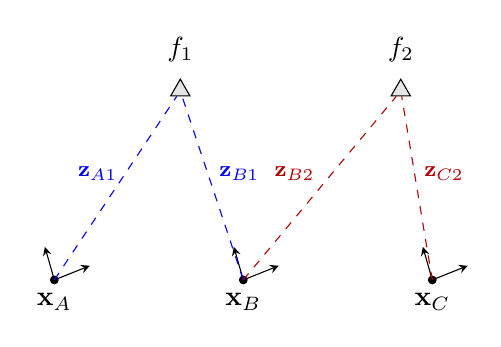
\begin{tikzpicture}[>=stealth,scale=1.0]
  % features (triangles) on top
  \node[draw,isosceles triangle,isosceles triangle apex angle=60,
        rotate=90,minimum size=6pt,inner sep=1pt,fill=black!10] (f1) at (1.6,2.4) {};
  \node[above] at (1.6,2.65) {$f_1$};
  \node[draw,isosceles triangle,isosceles triangle apex angle=60,
        rotate=90,minimum size=6pt,inner sep=1pt,fill=black!10] (f2) at (4.4,2.4) {};
  \node[above] at (4.4,2.65) {$f_2$};
  % poses (camera frames) on bottom
  \foreach \x/\nm in {0/A,2.4/B,4.8/C} {
    \fill (\x,0) circle (1.6pt);
    \draw[->] (\x,0) -- (\x+0.45,0.18);
    \draw[->] (\x,0) -- (\x-0.12,0.42);
    \node[below] at (\x,-0.05) {$\vect{x}_{\nm}$};
  }
  % observation rays
  \draw[blue,dashed] (0,0) -- (f1);          % A sees f1  (z_A1)
  \draw[blue,dashed] (2.4,0) -- (f1);        % B sees f1  (z_B1)
  \draw[red!70!black,dashed] (2.4,0) -- (f2);% B sees f2  (z_B2)
  \draw[red!70!black,dashed] (4.8,0) -- (f2);% C sees f2  (z_C2)
  \node[blue] at (0.55,1.35) {\footnotesize $\vect{z}_{A1}$};
  \node[blue] at (2.35,1.35) {\footnotesize $\vect{z}_{B1}$};
  \node[red!70!black] at (3.05,1.35) {\footnotesize $\vect{z}_{B2}$};
  \node[red!70!black] at (4.95,1.35) {\footnotesize $\vect{z}_{C2}$};
\end{tikzpicture}
\caption{Visual measurement graph: poses $\vect{x}_A,\vect{x}_B,\vect{x}_C$ observe features $f_1,f_2$. Each ray $\vect{z}_{(\cdot)}$ couples one pose to one feature, which determines the sparsity of $\vect{H}$ and of $\vect{\Sigma}=\vect{H}\trans\vect{H}$.}
\label{fig:lec04-factorgraph}
\end{figure}

The information matrix $\vect{\Sigma} = \vect{H}\trans\vect{H}$ has a block-sparse structure (a block $(i,j)$ is nonzero only when states $i$ and $j$ are co-observed in some measurement), shown in Fig.~\ref{fig:lec04-infomat}. Partitioning into poses $p=\{A,B,C\}$ and features $f=\{f_1,f_2\}$,
\begin{align}
\vect{\Sigma} = \vect{H}\trans\vect{H} \;\triangleq\;
\begin{bmatrix} \vect{\Sigma}_{pp} & \vect{\Sigma}_{pf} \\ \vect{\Sigma}_{pf}\trans & \vect{\Sigma}_{ff} \end{bmatrix}.
\end{align}

\begin{figure}[H]
\centering
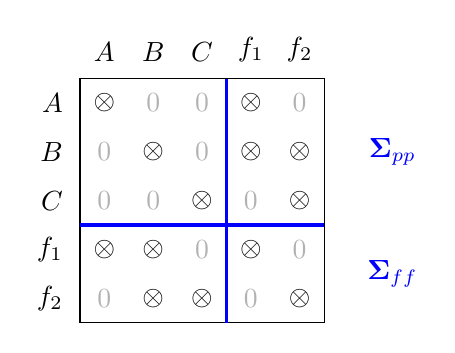
\begin{tikzpicture}[scale=0.62]
  % 5x5 grid of blocks: order A,B,C,f1,f2  (row 1 = top)
  \def\nz{{
    {1,0,0,1,0},
    {0,1,0,1,1},
    {0,0,1,0,1},
    {1,1,0,1,0},
    {0,1,1,0,1}}}
  \foreach \r in {0,...,4} {
    \foreach \c in {0,...,4} {
      \pgfmathparse{\nz[\r][\c]}
      \ifnum\pgfmathresult=1
        \node at (\c+0.5,4.5-\r) {$\otimes$};
      \else
        \node[gray!60] at (\c+0.5,4.5-\r) {$0$};
      \fi
    }
  }
  \draw (0,0) rectangle (5,5);
  % partition lines pose|feature at index 3
  \draw[blue,very thick] (3,0) -- (3,5);
  \draw[blue,very thick] (0,2) -- (5,2);
  % row / column labels
  \foreach \i/\nm in {0/A,1/B,2/C,3/f_1,4/f_2} {
    \node[left] at (-0.15,4.5-\i) {$\nm$};
    \node[above] at (\i+0.5,5.15) {$\nm$};
  }
  % block labels
  \node[blue] at (6.4,3.5) {$\vect{\Sigma}_{pp}$};
  \node[blue] at (6.4,1.0) {$\vect{\Sigma}_{ff}$};
\end{tikzpicture}
\caption{Sparsity of $\vect{\Sigma}=\vect{H}\trans\vect{H}$ ($\otimes$: nonzero block). The pose--pose block $\vect{\Sigma}_{pp}$ is block-diagonal, while $\vect{\Sigma}_{pf}$ records exactly which pose sees which feature. The information matrix reflects the problem structure.}
\label{fig:lec04-infomat}
\end{figure}

% =====================================================================
\subsection{A typical visual-odometry / SLAM pipeline}

How do the previous two lectures fit together into a working monocular system? A common pipeline incrementally grows poses $C_1,C_2,\dots$ and features $f_1,f_2,\dots$ (Fig.~\ref{fig:lec04-pipeline}):
\begin{enumerate}[label=(\arabic*),noitemsep,topsep=2pt]
\item \textbf{5-point algorithm} on $C_1,C_2$: recover ${}^{C_1}_{C_2}\vect{R}$ and ${}^{C_1}\vect{p}_{C_2}^{*}$ (up to scale).
\item \textbf{Feature triangulation}: with the recovered relative pose, triangulate $f_1,f_2,\dots$.
\item \textbf{P3P / PnP} for $C_3$: with known features, solve ${}^{C_1}_{C_3}\vect{R},\,{}^{C_1}\vect{p}_{C_3}$ (then triangulate new features).
\item \textbf{5-point or P3P/PnP} for $C_4$: solve ${}^{C_1}_{C_4}\vect{R},\,{}^{C_1}\vect{p}_{C_4}$.
\item \textbf{Bundle adjustment (BA)} over $C_1,C_2,C_3$ and $f_1,f_2,f_3,\dots$ (joint refinement of poses and structure).
\item \textbf{BA} extended to $C_1,C_2,C_3,C_4$ and $f_1,f_2,f_3,\dots$ as the window grows.
\item \textbf{Marginalization}: when there are too many poses ($C_1,\dots,C_n$) and features ($f_1,\dots,f_m$), marginalize old states $C_1,f_1,\dots$ to keep the system light-weight.
\end{enumerate}

\begin{figure}[H]
\centering
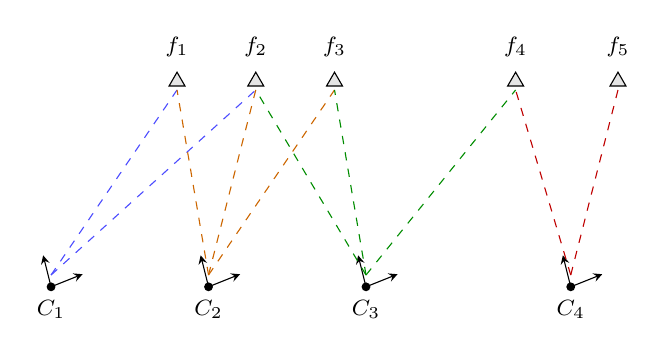
\begin{tikzpicture}[>=stealth,scale=1.0]
  % features (triangles) along the top
  \foreach \x/\nm in {2.0/f_1,3.0/f_2,4.0/f_3,6.3/f_4,7.6/f_5} {
    \node[draw,isosceles triangle,isosceles triangle apex angle=60,
          rotate=90,minimum size=5pt,inner sep=1pt,fill=black!10] at (\x,2.6) {};
    \node[above] at (\x,2.8) {\footnotesize $\nm$};
  }
  % camera frames along the bottom
  \foreach \x/\nm in {0.4/C_1,2.4/C_2,4.4/C_3,7.0/C_4} {
    \fill (\x,0) circle (1.6pt);
    \draw[->] (\x,0) -- (\x+0.4,0.16);
    \draw[->] (\x,0) -- (\x-0.1,0.40);
    \node[below] at (\x,-0.05) {\footnotesize $\nm$};
  }
  % a few observation rays (dashed, multi-color to suggest tracks)
  \draw[blue!70,dashed]   (0.4,0.15) -- (2.0,2.5);
  \draw[blue!70,dashed]   (0.4,0.15) -- (3.0,2.5);
  \draw[orange!80!black,dashed] (2.4,0.15) -- (2.0,2.5);
  \draw[orange!80!black,dashed] (2.4,0.15) -- (3.0,2.5);
  \draw[orange!80!black,dashed] (2.4,0.15) -- (4.0,2.5);
  \draw[green!55!black,dashed]  (4.4,0.15) -- (3.0,2.5);
  \draw[green!55!black,dashed]  (4.4,0.15) -- (4.0,2.5);
  \draw[green!55!black,dashed]  (4.4,0.15) -- (6.3,2.5);
  \draw[red!75!black,dashed]    (7.0,0.15) -- (6.3,2.5);
  \draw[red!75!black,dashed]    (7.0,0.15) -- (7.6,2.5);
\end{tikzpicture}
\caption{A monocular VO/SLAM pipeline grows poses $C_1,\dots,C_4$ and features $f_1,\dots,f_5$: bootstrap with the 5-point algorithm + triangulation, extend new poses with P3P/PnP, refine with bundle adjustment, and marginalize old states to bound cost. Combined with the previous two lectures, this builds up visual SLAM.}
\label{fig:lec04-pipeline}
\end{figure}

% =====================================================================
\subsection{Designing estimators: many ways to handle \texorpdfstring{$\vect{z}=\vect{h}(\vect{x})+\vect{n}$}{z=h(x)+n}}

Given $\vect{z} = \vect{h}(\vect{x}) + \vect{n}$, $\vect{n}\sim\mathcal{N}(\vect{0},\vect{R})$, there are many ways to linearize and solve, each leading to a different family of algorithms.

\paragraph{(1) Iterated re-linearization (GN / LM).} The typical solution $\min_{\vect{x}}\norm{\vect{z}-\vect{h}(\vect{x})}_{\vect{R}}^{2}$. Given a linearization $\hat{\vect{x}}$, $\tilde{\vect{z}} = \vect{H}\tilde{\vect{x}} + \vect{n}$; update $\vect{x}^{\oplus} = \hat{\vect{x}} + \tilde{\vect{x}}$, then \emph{redo} the linearization $\tilde{\vect{z}} = \vect{H}^{\oplus}\tilde{\vect{x}} + \vect{n}$ (Gauss--Newton or Levenberg--Marquardt).

\paragraph{(2) Linearize once + residual correction (FEJ).} What if we linearize only once, at a fixed $\hat{\vect{x}}^{0}$? With $\vect{H}^{0} = \vect{H}|_{\hat{\vect{x}}^{0}}$,
\begin{align}
\vect{z} &= \vect{h}(\hat{\vect{x}}^{0}) + \vect{H}^{0}(\vect{x}-\hat{\vect{x}}^{0}) + \vect{n} \\
\vect{z} - \vect{h}(\hat{\vect{x}}^{0}) &= \vect{H}^{0}\big(\vect{x} - \hat{\vect{x}} + \underbrace{\hat{\vect{x}} - \hat{\vect{x}}^{0}}_{\Delta\vect{x}}\big) + \vect{n}
= \vect{H}^{0}\tilde{\vect{x}} + \vect{H}^{0}\Delta\vect{x} + \vect{n},
\end{align}
so moving the known offset to the left gives the \emph{residual correction}
\begin{align}
\underbrace{\vect{z} - \vect{h}(\hat{\vect{x}}^{0})}_{\tilde{\vect{z}}^{0}} - \vect{H}^{0}\Delta\vect{x} = \vect{H}^{0}\tilde{\vect{x}} + \vect{n}.
\end{align}
Keeping the Jacobian fixed at the first estimate is \textbf{FEJ} (first-estimate Jacobians)~\cite{Huang2008ISER}, used e.g.\ in OKVIS~\cite{Leutenegger2014IJRR}; it preserves the correct observability/nullspace structure.

\paragraph{(3) Partial linearization (preintegration / iSAM).} For $\vect{x} = [\vect{x}_A\trans,\vect{x}_B\trans]\trans$, $\vect{z} = \vect{h}(\vect{x}_A,\vect{x}_B)+\vect{n}$, linearize only in $\vect{x}_B$ (about $\hat{\vect{x}}_B^{0}$) while keeping $\vect{x}_A$ exact:
\begin{align}
\vect{z} &= \vect{h}(\hat{\vect{x}}_A,\hat{\vect{x}}_B^{0}) + \vect{H}_A\tilde{\vect{x}}_A + \vect{H}_B^{0}\tilde{\vect{x}}_B + \vect{H}_B^{0}\Delta\vect{x}_B + \vect{n}, \\
\underbrace{\vect{z} - \vect{h}(\hat{\vect{x}}_A,\hat{\vect{x}}_B^{0})}_{\tilde{\vect{z}}^{0}} - \vect{H}_B^{0}\Delta\vect{x}_B
&= \begin{bmatrix} \vect{H}_A & \vect{H}_B^{0} \end{bmatrix}\begin{bmatrix} \tilde{\vect{x}}_A \\ \tilde{\vect{x}}_B \end{bmatrix} + \vect{n}.
\end{align}
This is the idea behind IMU \textbf{pre-integration}~\cite{Forster2017tro} and \textbf{ACI} (analytic combined integration)~\cite{Eckenhoff2017ICRA}; \textbf{iSAM}~\cite{Kaess2012IJRR} uses a similar partial-relinearization idea.

\paragraph{(4) Nullspace projection (MSCKF / structureless).} For $\vect{x}=[\vect{x}_A\trans,\vect{x}_B\trans]\trans$, $\tilde{\vect{z}} = \vect{H}_A\tilde{\vect{x}}_A + \vect{H}_B\tilde{\vect{x}}_B + \vect{n}$. If we find $\vect{N}$ with $\vect{N}\trans\vect{H}_B = \vect{0}$, then projecting onto the left nullspace removes $\vect{x}_B$:
\begin{align}
\vect{N}\trans\tilde{\vect{z}} = \vect{N}\trans\vect{H}_A\tilde{\vect{x}}_A + \cancel{\vect{N}\trans\vect{H}_B\tilde{\vect{x}}_B} + \vect{N}\trans\vect{n}.
\end{align}
This is the \textbf{MSCKF}~\cite{Mourikis2007ICRA} (multi-state constraint Kalman filter), a.k.a.\ the smart / structure-less vision factor: the features are eliminated without ever being added to the state.

\paragraph{(5) Invariant errors.} Instead of $\vect{x} = \hat{\vect{x}} + \tilde{\vect{x}}$, put $\vect{x}$ on a group $SE(3)$ / $SE_2(3)$ and use a right-invariant error,
\begin{align}
\vect{x} = \hat{\vect{x}}\boxplus\tilde{\vect{x}} = \Exp(\tilde{\vect{x}})\cdot\hat{\vect{x}} \;\Rightarrow\; \text{invariant SLAM / VIO}.
\end{align}

\paragraph{(6) Decoupled (right-)invariant errors.} For $\vect{x}=[\vect{x}_A\trans,\vect{x}_B\trans]\trans$, mix error types per block:
\begin{align}
\begin{cases}
\vect{x}_A = \hat{\vect{x}}_A\boxplus\tilde{\vect{x}}_A = \Exp(\tilde{\vect{x}}_A)\cdot\hat{\vect{x}}_A & \text{(group / invariant error)} \\
\vect{x}_B = \hat{\vect{x}}_B + \tilde{\vect{x}}_B & \text{(vector error)}
\end{cases}
\end{align}
which gives decoupled right-invariant SLAM / VIO.

\begin{quote}
Use your imagination to deal with $\big\{\vect{z}=\vect{h}(\vect{x})+\vect{n},\;\tilde{\vect{z}}=\vect{H}\tilde{\vect{x}}+\vect{n}\big\}$ to design different algorithms.
\end{quote}

% =====================================================================
\subsection{Designing a common system: from MAP to the EKF}

Consider the canonical prior + motion + measurement system
\begin{align}
\begin{cases}
\vect{x}_0 \sim \mathcal{N}(\hat{\vect{x}}_0,\vect{P}_0) & \to \text{prior} \\
\vect{x}_1 = \vect{f}(\vect{x}_0) + \vect{w}_0, \quad \vect{w}_k\sim\mathcal{N}(\vect{0},\vect{Q}) & \to \text{motion model} \\
\vect{z}_1 = \vect{h}(\vect{x}_1) + \vect{n}_1, \quad \vect{n}_1\sim\mathcal{N}(\vect{0},\vect{R}) & \to \text{measurement model}
\end{cases}
\end{align}
The MAP estimate factorizes by Bayes' rule,
\begin{align}
\max_{\vect{x}} p(\vect{x}\mid\vect{z})
= \max_{\vect{x}} \frac{p(\vect{z}\mid\vect{x})\,p(\vect{x})}{p(\vect{z})}
= \max_{\vect{x}} \frac{p(\vect{z}_1\mid\vect{x}_1)\,p(\vect{x}_1\mid\vect{x}_0)\,p(\vect{x}_0)}{p(\vect{z})},
\end{align}
which is equivalent to the nonlinear least-squares cost
\begin{align}
\min_{\vect{x}} \;\norm{\vect{z}_1 - \vect{h}(\vect{x}_1)}_{\vect{R}}^{2}
+ \norm{\vect{x}_1 - \vect{f}(\vect{x}_0)}_{\vect{Q}}^{2}
+ \norm{\vect{x}_0 - \hat{\vect{x}}_0}_{\vect{P}_0}^{2}.
\end{align}
There are two ways to solve it:
\begin{enumerate}[label=\arabic*.,noitemsep,topsep=2pt]
\item \textbf{Batch:} minimize all three terms jointly $\Rightarrow \hat{\vect{x}}_1,\vect{P}_1$.
\item \textbf{Incremental:}
  \begin{enumerate}[label=(\roman*),noitemsep,topsep=1pt]
  \item handle the prior + motion terms $\norm{\vect{x}_0-\hat{\vect{x}}_0}_{\vect{P}_0}^{2} + \norm{\vect{x}_1-\vect{f}(\vect{x}_0)}_{\vect{Q}}^{2}$;
  \item marginalize $\vect{x}_0$, keep $\vect{x}_1$, giving $(\hat{\vect{x}}_{1|0},\vect{P}_{1|0})$;
  \item add the measurement $\norm{\vect{x}_1-\hat{\vect{x}}_{1|0}}_{\vect{P}_{1|0}}^{2} + \norm{\vect{z}_1-\vect{h}(\vect{x}_1)}_{\vect{R}}^{2} \Rightarrow \hat{\vect{x}}_1,\vect{P}_1$.
  \end{enumerate}
\end{enumerate}
The incremental route is exactly the EKF predict/update, as we now derive.

\paragraph{Propagation (marginalize $\vect{x}_0$).} Linearize the motion model, $\vect{x}_1 = \vect{f}(\vect{x}_0)+\vect{w}_0 \Rightarrow \hat{\vect{x}}_1 + \tilde{\vect{x}}_1 = \vect{f}(\hat{\vect{x}}_0) + \vect{F}\tilde{\vect{x}}_0 + \vect{w}_0$, and define the motion residual
\begin{align}
\vect{r}_{\vect{x}} \triangleq \hat{\vect{x}}_1 - \vect{f}(\hat{\vect{x}}_0) = \vect{F}\tilde{\vect{x}}_0 - \tilde{\vect{x}}_1 + \vect{w}_0,
\qquad
\vect{w}_0 = \vect{r}_{\vect{x}} - \begin{bmatrix} \vect{F} & -\vect{I} \end{bmatrix}\begin{bmatrix} \tilde{\vect{x}}_0 \\ \tilde{\vect{x}}_1 \end{bmatrix}.
\end{align}
The prior + motion cost (writing $\vect{Q}_0=\vect{Q}$) is
\begin{align}
\min \; \norm{\tilde{\vect{x}}_0}_{\vect{P}_0}^{2}
+ \Big\|\,\vect{r}_{\vect{x}} - \begin{bmatrix} \vect{F} & -\vect{I} \end{bmatrix}\begin{bmatrix} \tilde{\vect{x}}_0 \\ \tilde{\vect{x}}_1 \end{bmatrix}\Big\|_{\vect{Q}_0}^{2}.
\end{align}
Collecting quadratic and linear terms, the cost $C$ is
\begin{align}
C = \begin{bmatrix} \tilde{\vect{x}}_0 \\ \tilde{\vect{x}}_1 \end{bmatrix}\trans
\begin{bmatrix} \vect{P}_0^{-1} + \vect{F}\trans\vect{Q}_0^{-1}\vect{F} & -\vect{F}\trans\vect{Q}_0^{-1} \\ -\vect{Q}_0^{-1}\vect{F} & \vect{Q}_0^{-1} \end{bmatrix}
\begin{bmatrix} \tilde{\vect{x}}_0 \\ \tilde{\vect{x}}_1 \end{bmatrix}
- 2\begin{bmatrix} \tilde{\vect{x}}_0 \\ \tilde{\vect{x}}_1 \end{bmatrix}\trans
\begin{bmatrix} \vect{F}\trans \\ -\vect{I} \end{bmatrix}\vect{Q}_0^{-1}\vect{r}_{\vect{x}}
+ \vect{r}_{\vect{x}}\trans\vect{Q}_0^{-1}\vect{r}_{\vect{x}}.
\end{align}
Setting $\partial C/\partial[\tilde{\vect{x}}_0;\tilde{\vect{x}}_1] = \vect{0}$ gives the information system
\begin{align}
\begin{bmatrix} \vect{P}_0^{-1} + \vect{F}\trans\vect{Q}_0^{-1}\vect{F} & -\vect{F}\trans\vect{Q}_0^{-1} \\ -\vect{Q}_0^{-1}\vect{F} & \vect{Q}_0^{-1} \end{bmatrix}
\begin{bmatrix} \tilde{\vect{x}}_0 \\ \tilde{\vect{x}}_1 \end{bmatrix}
= \begin{bmatrix} \vect{F}\trans\vect{Q}_0^{-1}\vect{r}_{\vect{x}} \\ -\vect{Q}_0^{-1}\vect{r}_{\vect{x}} \end{bmatrix}.
\end{align}
Marginalizing $\vect{x}_0$ (Schur complement onto the $\vect{x}_1$ block) and applying the matrix inversion lemma,
\begin{align}
\Big[\vect{Q}_0^{-1} - \vect{Q}_0^{-1}\vect{F}\big(\vect{P}_0^{-1} + \vect{F}\trans\vect{Q}_0^{-1}\vect{F}\big)^{-1}\vect{F}\trans\vect{Q}_0^{-1}\Big]\tilde{\vect{x}}_1
&= -\vect{Q}_0^{-1}\vect{r}_{\vect{x}} + \vect{Q}_0^{-1}\vect{F}\big(\vect{P}_0^{-1}+\vect{F}\trans\vect{Q}_0^{-1}\vect{F}\big)^{-1}\vect{F}\trans\vect{Q}_0^{-1}\vect{r}_{\vect{x}}, \notag \\
\underbrace{\big(\vect{Q}_0 + \vect{F}\vect{P}_0\vect{F}\trans\big)^{-1}}_{\vect{P}_{1|0}^{-1}}\tilde{\vect{x}}_1
&= -\big(\vect{Q}_0 + \vect{F}\vect{P}_0\vect{F}\trans\big)^{-1}\vect{r}_{\vect{x}}.
\end{align}
This is the EKF \textbf{propagation}: the predicted covariance and mean are
\begin{empheq}[box=\fbox]{align}
\vect{P}_{1|0} = \vect{F}\vect{P}_0\vect{F}\trans + \vect{Q}_0, \qquad
\hat{\vect{x}}_{1|0} = \vect{f}(\hat{\vect{x}}_0) \;\;(\text{i.e.\ }\vect{r}_{\vect{x}}=\vect{0}).
\end{empheq}

\paragraph{Update (add the measurement).} Now include the measurement $\vect{z}_1 = \vect{h}(\vect{x}_1)+\vect{n}\Rightarrow\tilde{\vect{z}}=\vect{H}\tilde{\vect{x}}_1+\vect{n}$. The full cost
\begin{align}
\norm{\tilde{\vect{z}} - \vect{H}\tilde{\vect{x}}_1}_{\vect{R}}^{2}
+ \Big\|\vect{r}_{\vect{x}} - \begin{bmatrix}\vect{F} & -\vect{I}\end{bmatrix}\begin{bmatrix}\tilde{\vect{x}}_0\\\tilde{\vect{x}}_1\end{bmatrix}\Big\|_{\vect{Q}_0}^{2}
+ \norm{\tilde{\vect{x}}_0}_{\vect{P}_0}^{2}
\end{align}
yields the augmented information system (the measurement adds $\vect{H}\trans\vect{R}^{-1}\vect{H}$ to the $\vect{x}_1$ block and $\vect{H}\trans\vect{R}^{-1}\tilde{\vect{z}}$ to its residual),
\begin{align}
\begin{bmatrix} \vect{P}_0^{-1} + \vect{F}\trans\vect{Q}_0^{-1}\vect{F} & -\vect{F}\trans\vect{Q}_0^{-1} \\ -\vect{Q}_0^{-1}\vect{F} & \vect{Q}_0^{-1} + \vect{H}\trans\vect{R}^{-1}\vect{H} \end{bmatrix}
\begin{bmatrix} \tilde{\vect{x}}_0 \\ \tilde{\vect{x}}_1 \end{bmatrix}
= \begin{bmatrix} \vect{F}\trans\vect{Q}_0^{-1}\vect{r}_{\vect{x}} \\ -\vect{Q}_0^{-1}\vect{r}_{\vect{x}} + \vect{H}\trans\vect{R}^{-1}\tilde{\vect{z}} \end{bmatrix}.
\end{align}
Marginalizing $\vect{x}_0$ again and recognizing $\vect{P}_{1|0}^{-1} = (\vect{Q}_0+\vect{F}\vect{P}_0\vect{F}\trans)^{-1}$,
\begin{align}
\underbrace{\big(\vect{H}\trans\vect{R}^{-1}\vect{H} + \vect{P}_{1|0}^{-1}\big)}_{\vect{\Sigma}\,=\,\vect{P}_{1|1}^{-1}}\tilde{\vect{x}}_1
= \vect{H}\trans\vect{R}^{-1}\tilde{\vect{z}} - \underbrace{\vect{P}_{1|0}^{-1}\vect{r}_{\vect{x}}}_{\to\,\vect{0}}.
\end{align}
After propagation $\vect{r}_{\vect{x}}=\vect{0}$, so the second term drops. Applying the matrix inversion lemma to the updated covariance,
\begin{align}
\vect{P}_{1|1} = \big(\vect{P}_{1|0}^{-1} + \vect{H}\trans\vect{R}^{-1}\vect{H}\big)^{-1}
= \vect{P}_{1|0} - \vect{P}_{1|0}\vect{H}\trans\big(\vect{H}\vect{P}_{1|0}\vect{H}\trans + \vect{R}\big)^{-1}\vect{H}\vect{P}_{1|0},
\end{align}
and for the mean correction, using the same lemma to convert information $\to$ covariance form,
\begin{align}
\tilde{\vect{x}}_1
&= \big(\vect{P}_{1|0}^{-1} + \vect{H}\trans\vect{R}^{-1}\vect{H}\big)^{-1}\vect{H}\trans\vect{R}^{-1}\tilde{\vect{z}} \\
&= \Big(\vect{P}_{1|0} - \vect{P}_{1|0}\vect{H}\trans\big(\vect{H}\vect{P}_{1|0}\vect{H}\trans+\vect{R}\big)^{-1}\vect{H}\vect{P}_{1|0}\Big)\vect{H}\trans\vect{R}^{-1}\tilde{\vect{z}} \\
&= \vect{P}_{1|0}\vect{H}\trans\Big(\vect{R}^{-1} - \big(\vect{H}\vect{P}_{1|0}\vect{H}\trans+\vect{R}\big)^{-1}\vect{H}\vect{P}_{1|0}\vect{H}\trans\vect{R}^{-1}\Big)\tilde{\vect{z}} \\
&= \vect{P}_{1|0}\vect{H}\trans\big(\vect{H}\vect{P}_{1|0}\vect{H}\trans+\vect{R}\big)^{-1}\Big(\big(\vect{H}\vect{P}_{1|0}\vect{H}\trans+\vect{R}\big)\vect{R}^{-1} - \vect{H}\vect{P}_{1|0}\vect{H}\trans\vect{R}^{-1}\Big)\tilde{\vect{z}} \\
&= \vect{P}_{1|0}\vect{H}\trans\big(\vect{H}\vect{P}_{1|0}\vect{H}\trans+\vect{R}\big)^{-1}\tilde{\vect{z}}.
\end{align}
Finally, with the Kalman gain $\vect{K} = \vect{P}_{1|0}\vect{H}\trans(\vect{H}\vect{P}_{1|0}\vect{H}\trans+\vect{R})^{-1}$, we recover the EKF \textbf{update}:
\begin{empheq}[box=\fbox]{align}
\tilde{\vect{x}}_1 = \vect{P}_{1|0}\vect{H}\trans\big(\vect{H}\vect{P}_{1|0}\vect{H}\trans+\vect{R}\big)^{-1}\tilde{\vect{z}}, \qquad
\vect{P}_{1|1} = \vect{P}_{1|0} - \vect{P}_{1|0}\vect{H}\trans\big(\vect{H}\vect{P}_{1|0}\vect{H}\trans+\vect{R}\big)^{-1}\vect{H}\vect{P}_{1|0}.
\end{empheq}
The extended Kalman filter is thus the incremental (marginalize-then-update) solution of the same MAP problem that batch least squares solves jointly --- the two views are connected by the matrix inversion lemma and the Schur complement.

% =====================================================================
\subsection{The relationship between Schur complement and nullspace projection}

The Schur-complement marginalization (\S4.3) and the nullspace projection (\S4.6, item~4, the MSCKF) both eliminate $\vect{x}_B$ --- it turns out they are the \emph{same} operation. Take $\vect{z} = \vect{h}(\vect{x}_A,\vect{x}_B) + \vect{n}$, $\vect{n}\sim\mathcal{N}(\vect{0},\vect{R})$, with $\tilde{\vect{z}} = \vect{H}_A\tilde{\vect{x}}_A + \vect{H}_B\tilde{\vect{x}}_B + \vect{n}$.

\paragraph{(1) Information form.} The normal equations are
\begin{align}
\begin{bmatrix} \vect{H}_A\trans\vect{R}^{-1}\vect{H}_A & \vect{H}_A\trans\vect{R}^{-1}\vect{H}_B \\ \vect{H}_B\trans\vect{R}^{-1}\vect{H}_A & \vect{H}_B\trans\vect{R}^{-1}\vect{H}_B \end{bmatrix}
\begin{bmatrix} \tilde{\vect{x}}_A \\ \tilde{\vect{x}}_B \end{bmatrix}
= \begin{bmatrix} \vect{H}_A\trans \\ \vect{H}_B\trans \end{bmatrix}\vect{R}^{-1}\tilde{\vect{z}}.
\end{align}
Marginalizing $\vect{x}_B$ and keeping $\vect{x}_A$ via the Schur complement gives
\begin{empheq}[box=\fbox]{align}
\underbrace{\big(\vect{H}_A\trans\vect{R}^{-1}\vect{H}_A - \vect{H}_A\trans\vect{R}^{-1}\vect{H}_B(\vect{H}_B\trans\vect{R}^{-1}\vect{H}_B)^{-1}\vect{H}_B\trans\vect{R}^{-1}\vect{H}_A\big)}_{\text{information}}\tilde{\vect{x}}_A & \notag\\
= \underbrace{\vect{H}_A\trans\vect{R}^{-1}\tilde{\vect{z}} - \vect{H}_A\trans\vect{R}^{-1}\vect{H}_B(\vect{H}_B\trans\vect{R}^{-1}\vect{H}_B)^{-1}\vect{H}_B\trans\vect{R}^{-1}\tilde{\vect{z}}}_{\text{residual}}&. \tag{Eq.\ 1}
\end{empheq}

\paragraph{(2) Nullspace form.} Take a (thin) QR-type factorization of $\vect{H}_B$,
\begin{align}
\vect{H}_B = \begin{bmatrix} \vect{Q}_e & \vect{Q}_N \end{bmatrix}\begin{bmatrix} \vect{U} \\ \vect{0} \end{bmatrix} = \vect{Q}_e\vect{U} + \vect{Q}_N\cdot\vect{0} = \vect{Q}_e\vect{U},
\end{align}
with $\vect{U}$ upper triangular and $[\vect{Q}_e\;\vect{Q}_N]$ orthogonal, so $\vect{Q}_e\vect{Q}_e\trans + \vect{Q}_N\vect{Q}_N\trans = \vect{I}$, $\vect{Q}_e\trans\vect{Q}_e = \vect{I}$, $\vect{Q}_N\trans\vect{Q}_N = \vect{I}$, and the left nullspace satisfies $\vect{Q}_N\trans\vect{H}_B = \vect{Q}_N\trans\vect{Q}_e\vect{U} = \vect{0}$. Projecting the residual onto $\vect{Q}_N$ removes $\vect{x}_B$:
\begin{align}
\vect{Q}_N\trans\tilde{\vect{z}} = \vect{Q}_N\trans\vect{H}_A\tilde{\vect{x}}_A + \cancel{\vect{Q}_N\trans\vect{H}_B\tilde{\vect{x}}_B} + \vect{Q}_N\trans\vect{n}
= \vect{Q}_N\trans\vect{H}_A\tilde{\vect{x}}_A + \vect{Q}_N\trans\vect{n},
\end{align}
with projected noise covariance $\vect{Q}_N\trans\vect{R}\vect{Q}_N$. The resulting normal equations are
\begin{empheq}[box=\fbox]{align}
(\vect{Q}_N\trans\vect{H}_A)\trans(\vect{Q}_N\trans\vect{R}\vect{Q}_N)^{-1}(\vect{Q}_N\trans\vect{H}_A)\,\tilde{\vect{x}}_A
= (\vect{Q}_N\trans\vect{H}_A)\trans(\vect{Q}_N\trans\vect{R}\vect{Q}_N)^{-1}\vect{Q}_N\trans\tilde{\vect{z}}. \tag{Eq.\ 2}
\end{empheq}

\paragraph{Are Eq.~1 and Eq.~2 equivalent?} Consider the isotropic case $\vect{R} = \sigma^2\vect{I}$. With $\vect{H}_B = \vect{Q}_e\vect{U}$,
\begin{align}
\vect{H}_B\trans\vect{R}^{-1}\vect{H}_B = (\vect{Q}_e\vect{U})\trans\frac{\vect{I}}{\sigma^2}\vect{Q}_e\vect{U} = \frac{\vect{U}\trans\vect{U}}{\sigma^2},
\end{align}
so the projector that appears in the Schur complement of Eq.~1 is
\begin{align}
\vect{H}_A\trans\vect{R}^{-1}\vect{H}_B(\vect{H}_B\trans\vect{R}^{-1}\vect{H}_B)^{-1}\vect{H}_B\trans\vect{R}^{-1}\vect{H}_A
&= \vect{H}_A\trans\frac{\vect{I}}{\sigma^2}\vect{Q}_e\vect{U}\,\sigma^2(\vect{U}\trans\vect{U})^{-1}\vect{U}\trans\vect{Q}_e\trans\frac{\vect{I}}{\sigma^2}\vect{H}_A \notag\\
&= \frac{1}{\sigma^2}\vect{H}_A\trans\vect{Q}_e\vect{Q}_e\trans\vect{H}_A.
\end{align}
Hence the Eq.~1 information becomes, using $\vect{Q}_e\vect{Q}_e\trans = \vect{I} - \vect{Q}_N\vect{Q}_N\trans$,
\begin{align}
\frac{1}{\sigma^2}\vect{H}_A\trans\vect{H}_A - \frac{1}{\sigma^2}\vect{H}_A\trans\vect{Q}_e\vect{Q}_e\trans\vect{H}_A
= \frac{1}{\sigma^2}\vect{H}_A\trans\big(\vect{I} - \vect{Q}_e\vect{Q}_e\trans\big)\vect{H}_A
= \frac{1}{\sigma^2}\vect{H}_A\trans\vect{Q}_N\vect{Q}_N\trans\vect{H}_A.
\end{align}
The Eq.~2 information, using $\vect{Q}_N\trans\vect{R}\vect{Q}_N = \sigma^2\vect{Q}_N\trans\vect{Q}_N = \sigma^2\vect{I}$, is
\begin{align}
(\vect{Q}_N\trans\vect{H}_A)\trans(\sigma^2\vect{I})^{-1}(\vect{Q}_N\trans\vect{H}_A) = \frac{1}{\sigma^2}\vect{H}_A\trans\vect{Q}_N\vect{Q}_N\trans\vect{H}_A,
\end{align}
which is identical (the residuals match the same way). Therefore, for isotropic noise, Schur-complement marginalization and left-nullspace projection produce exactly the same information and residual --- the MSCKF's structureless update is precisely the marginalization of the feature.




%%%%%%%%%%%%%%%%%%%%%%%%%%%%%%%%%%%%%%%%%%%%%%%%%%%%%%%%%%%%%%%%%%%%%%%
% Append our bibliography
%%%%%%%%%%%%%%%%%%%%%%%%%%%%%%%%%%%%%%%%%%%%%%%%%%%%%%%%%%%%%%%%%%%%%%%
%
\addcontentsline{toc}{section}{References}
\printbibliography
\newpage

%
\end{document}
\grid
\grid
